%\documentclass[anon,12pt]{colt2018} % Anonymized submission
\documentclass[final,12pt]{colt2018} % Include author names

% The following packages will be automatically loaded:
% amsmath, amssymb, natbib, graphicx, url, algorithm2e


\definecolor{pearOne}{HTML}{2C3E50}
%A9CF54
\definecolor{pearTwo}{HTML}{A9CF54}
\definecolor{pearTwoT}{HTML}{C2895B}
\definecolor{pearThree}{HTML}{E74C3C}
\colorlet{titleTh}{pearOne}
\colorlet{bull}{pearTwo}
\definecolor{pearcomp}{HTML}{B97E29}
\definecolor{pearFour}{HTML}{588F27}
\definecolor{pearFith}{HTML}{ECF0F1}
\definecolor{pearDark}{HTML}{2980B9}
\definecolor{pearDarker}{HTML}{1D2DEC}
%343653


\title[Best of both worlds: Stochastic \& adversarial
 best-arm identification]{\textcolor{pearOne}{Best of both worlds:} \\ \textcolor{pearDark}{Stochastic} 
 	\textcolor{pearOne}{\&} \textcolor{pearThree}{adversarial} 
 	 best-arm identification}
\usepackage{times}
 % Use \Name{Author Name} to specify the name.
 % If the surname contains spaces, enclose the surname
 % in braces, e.g. \Name{John {Smith Jones}} similarly
 % if the name has a "von" part, e.g \Name{Jane {de Winter}}.
 % If the first letter in the forenames is a diacritic
 % enclose the diacritic in braces, e.g. \Name{{\'E}louise Smith}

 % Two authors with the same address
  % \coltauthor{\Name{Author Name1} \Email{abc@sample.com}\and
  %  \Name{Author Name2} \Email{xyz@sample.com}\\
  %  \addr Address}

 % Three or more authors with the same address:
 % \coltauthor{\Name{Author Name1} \Email{an1@sample.com}\\
 %  \Name{Author Name2} \Email{an2@sample.com}\\
 %  \Name{Author Name3} \Email{an3@sample.com}\\
 %  \addr Address}


 %  Authors with different addresses:
\coltauthor{
	\!\!\Name{Yasin {Abbasi-Yadkori}} \Email{abbasiya@adobe.com}\\
	\addr Adobe Research, USA
	\AND
	\Name{Peter L. Bartlett} \Email{peter@berkeley.edu}\\
	\addr University of California, Berkeley, USA
		  \AND
 \Name{Victor Gabillon} \Email{victor.gabillon@qut.edu.au}\\
 \addr Queensland University of Technology - ACEMS, Australia
 \AND
 \Name{Alan Malek} \Email{amalek@mit.edu}\\
 \addr Massachusetts Institute of Technology, USA
 \AND
 \Name{Michal Valko} \Email{michal.valko@inria.fr}\\
 \addr SequeL team, INRIA Lille - Nord Europe, France
 }

\usepackage{mathtools}
\usepackage{hyperref}
\usepackage{bm}
\usepackage{xcolor}
%\usepackage{sty/notation}
\usepackage{wrapfig}
\usepackage{tikz}
\usepackage{algorithm}
\usepackage{algorithmic}
% Definitions of handy macros can go here

\usepackage{thm-restate}

\usepackage{colortbl}
\usepackage{caption} 
\usepackage{enumitem} 
\captionsetup[table]{skip=10pt}

\usepackage[colorinlistoftodos, textwidth=26mm, shadow]{todonotes}
\setlength{\marginparwidth}{2.5cm}

%% TODOs
% todo by Victor
\let\oldtodo\todo
\renewcommand{\todo}[1]{\oldtodo{\scriptsize #1}}
\newcommand{\todov}[1]{\oldtodo[color=yellow, inline]{\small #1}}
\newcommand{\todovout}[1]{\oldtodo[color=yellow]{\scriptsize #1}}
% todo by Alan
\newcommand{\todoa}[1]{\oldtodo[color=green, inline]{\small #1}}
\newcommand{\todoaout}[1]{\oldtodo[color=green]{\scriptsize #1}}
% todo by Michal
\newcommand{\todomi}[1]{\oldtodo[color=cyan, inline]{\small #1}}
\newcommand{\todom}[1]{\oldtodo[color=cyan]{\scriptsize #1}}


\newcounter{fpcounter}
%\renewcommand{\thefpcounter}{\thechapter.\arabic{fpcounter}}
%\renewcommand{\thefpcounter}{\thesection.\arabic{fpcounter}}
\renewcommand{\thefpcounter}{\arabic{fpcounter}}

\newenvironment{fp}[2]{%
\refstepcounter{fpcounter}%
\label{#1}%
\noindent{\raisebox{.04cm}{\textcolor{bull}{$\blacktriangleright$}} Experiment~\thefpcounter: }%
}%
{}%




% !TEX root = Main.tex
\let\inf\undefined

%\usepackage{xspace}
%\renewcommand{\textsc}[1]{\texttt{#1}}
\renewcommand{\ttdefault}{lmtt}

\DeclareMathOperator*{\inf}{\vphantom{\sup}inf}
\DeclareMathOperator*{\ex}{\mathbb E}
\DeclareMathOperator*{\tr}{tr}
\DeclareMathOperator*{\diag}{diag}
\DeclareMathOperator*{\supp}{supp}
\DeclareMathOperator*{\rank}{rank}
\DeclareMathOperator*{\conv}{conv}
\DeclareMathOperator*{\pr}{\mathbb P}
\DeclareBoldMathCommand{\I}{I}
\DeclareBoldMathCommand{\e}{e}
\DeclareBoldMathCommand{\f}{f}
\DeclareBoldMathCommand{\g}{g}
\DeclareBoldMathCommand{\a}{a}
\DeclareBoldMathCommand{\b}{b}
\DeclareBoldMathCommand{\c}{c}
\DeclareBoldMathCommand{\d}{d}
\DeclareBoldMathCommand{\m}{m}
\DeclareBoldMathCommand{\p}{p}
\DeclareBoldMathCommand{\q}{q}
\DeclareBoldMathCommand{\v}{v}
\DeclareBoldMathCommand{\V}{V}
\DeclareBoldMathCommand{\x}{x}
\DeclareBoldMathCommand{\t}{t}
\DeclareBoldMathCommand{\X}{X}
\DeclareBoldMathCommand{\Y}{Y}
\DeclareBoldMathCommand{\z}{z}
\DeclareBoldMathCommand{\Z}{Z}
\DeclareBoldMathCommand{\M}{M}
\DeclareBoldMathCommand{\n}{n}
\DeclareBoldMathCommand{\ssigma}{\sigma}
\DeclareBoldMathCommand{\SSigma}{\Sigma}
\DeclareBoldMathCommand{\OOmega}{\Omega}
\DeclareBoldMathCommand{\y}{y}
% \DeclareBoldMathCommand{\u}{u}  For some reason, this particular command doesn't work with the jmlr style file...
\DeclareBoldMathCommand{\U}{U}
\DeclareBoldMathCommand{\w}{w}
\DeclareBoldMathCommand{\W}{W}
\DeclareBoldMathCommand{\L}{L}

\DeclareBoldMathCommand{\s}{s}
\DeclareBoldMathCommand{\S}{S}
\DeclareBoldMathCommand{\A}{A}
\DeclareBoldMathCommand{\B}{B}
\DeclareBoldMathCommand{\C}{C}
\DeclareBoldMathCommand{\D}{D}
\DeclareBoldMathCommand{\E}{\mathbb{E}}
\DeclareBoldMathCommand{\G}{G}
\DeclareBoldMathCommand{\H}{H}
\DeclareBoldMathCommand{\P}{\mathbb{P}}
\DeclareBoldMathCommand{\Q}{Q}
\DeclareBoldMathCommand{\R}{R}
\DeclareBoldMathCommand{\X}{X}
\DeclareBoldMathCommand{\mmu}{\mu}
\DeclareBoldMathCommand{\ones}{1}
\DeclareBoldMathCommand{\zeros}{0}

\newcommand{\cO}{\mathcal{O}}
\newcommand{\tcO}{\widetilde{\cO}}
\newcommand{\OO}{\mathcal{O}}
\newcommand{\tOO}{\wt{\OO}}

\let\top\intercal
\newcommand{\Graph}{\mathcal G}
\newcommand{\indicator}[1]{\mathbf 1\{#1\}}

\newcommand{\Reals}{\mathbb R}
\newcommand{\Value}{\mathcal V}
\newcommand{\Regret}{\mathcal R}
\newcommand{\RefSet}{\mathcal U}

\newcommand{\gap}{\Delta}
\newcommand{\sample}{X}
\newcommand{\pulledArm}{I}
\newcommand{\nArms}{K}
\newcommand{\timeHorizon}{n}
\newcommand{\timeHorizonDeux}{n'}
\newcommand{\cumulGain}{G}
%\newcommand{\setArms}{A}
\newcommand{\setArms}{[\nArms]}
\newcommand{\mean}{\mu}
\newcommand{\gainVector}{\g}
\newcommand{\estGainVector}{\tilde\gainVector}
\newcommand{\estCumulGainVector}{\tilde\cumulGain}
\newcommand{\estBiasCumulGain}{\hat\cumulGain}
\newcommand{\recomArm}{J}
\newcommand{\bestArm}{k^\star}
\newcommand{\bestArmAd}{\bestArm_{\textsc{ADV}}}
\newcommand{\bestArmSto}{\bestArm_{\textsc{STO}}}
\newcommand{\learnerDist}{\p}
\newcommand{\pullsNumber}{T}
\newcommand{\advPro}{\textsc{ADV}}
\newcommand{\stoPro}{\textsc{STO}}
\newcommand{\basePro}{\textsc{BASE}}
\newcommand{\refarm}{\bar k}
\newcommand{\permu}{\sigma}

\newcommand{\dividefac}{a}
\newcommand{\matrixAd}{\X}



%\newcommand{\setArmsmo}{\setArms_{-1}}
\newcommand{\setArmsmo}{[2:\nArms]}
\newcommand{\earlyPhase}{L}
\newcommand{\SR}{{\normalfont \texttt{SR}}}
\newcommand{\hyperband}{{\normalfont \texttt{Hyperband}}}
\newcommand{\SH}{{\normalfont \texttt{SH}}}
\newcommand{\ARU}{\textsc{aru}}
\newcommand{\probaOne}{\normalfont \texttt{probaONE}}
\newcommand{\ProbabilityONE}{\normalfont \texttt{\textcolor[rgb]{0.5,0.2,0}{ProbabilityONE}}}
\newcommand{\RULE}{{\normalfont  \texttt{Rule}}}
%\newcommand{\RULE}{\texttt{Rule}}
\newcommand{\Unif}{{\normalfont \textsc{UNIF}}}
\newcommand{\Both}{{\normalfont \textsc{{BOB}}}}
\newcommand{\Pone}{{\normalfont \texttt{\textcolor[rgb]{0.5,0.2,0}{P1}}}}
\newcommand{\complexity}{H}
\newcommand{\complexitySR}{\complexity_{\SR}}
\newcommand{\complexityUnif}{\complexity_{\Unif}}
\newcommand{\complexityBoth}{\complexity_{\Both}}
\newcommand{\complexityProOne}{\complexity_{\Pone}}
\newcommand{\Exp}{\E}
\newcommand{\Pro}{\P}

\newcommand{\ProErr}{e}
\newcommand{\eventc}{\xi}
\newcommand{\eventu}{\xi}
\newcommand{\eventbob}{\xi}
\newcommand{\expectCumul}{M}

\newcommand{\sumlemma}{\bar G}
\newcommand{\pullearlyPhase}{\bar T}

\newcommand{\TODO}[1]{
\ifmmode
\text{\textcolor{red}{TODO: #1}}
\else
\textcolor{red}{TODO: #1}
\fi
}

\newcommand{\group}{C}
\newcommand{\referArm}{z}

\newcommand{\rankk}{r}
\newcommand{\upperRank}{\rankk^+}

\newcommand{\CommaBin}{\mathbin{\raisebox{0.5ex}{,}}}
\newcommand{\eps}{\varepsilon}
\renewcommand{\epsilon}{\varepsilon}
\renewcommand{\hat}{\widehat}
\renewcommand{\tilde}{\widetilde}
\renewcommand{\bar}{\overline}

\newcommand{\var}{\sigma^2}
\newcommand{\range}{b}


\newcommand{\bernPara}{\theta}
\newcommand{\lowBrv}{\ell}
\newcommand{\upBrv}{u}

\newcommand{\phaseTime}{n}
\newcommand{\propTime}{a}
\newcommand{\propTimeVec}{\a}
\newcommand{\propTimeVecSpa}{\A}

\newcommand{\Real}{\mathbb{R}}
\newcommand{\Integer}{\mathbb{N}}

\newcommand{\Gaps}{\boldsymbol{\Delta}}

\newcommand{\TphaseNumber}{p}
\newcommand{\phaseIndOne}{l}
\newcommand{\phaseIndTwo}{q}

\newcommand{\dataset}{{\cal D}}
\newcommand{\fracpartial}[2]{\frac{\partial #1}{\partial  #2}}
\newcommand{\argmax}{\mathrm{argmax}}
\newcommand{\argmin}{\mathrm{argmin}}
\newcommand{\matdata}{\A}
\newcommand{\horizon}{T}

% Heading arguments are {volume}{year}{pages}{submitted}{published}{author-full-names}

% Short headings should be running head and authors last namesm
\newcounter{scratchcounter}
\begin{document}

\maketitle

We present preconditioned stochastic gradient descent (SGD) algorithms for the $\ell_1$ minimization problem $\min_{\xx}\|\AA \xx - \bb\|_1$ in the overdetermined case, where there are far more constraints than variables. Specifically, we have $\AA \in \R^{n \times d}$ for $n \gg d$. Commonly known as the Least Absolute Deviations problem, $\ell_1$ regression can be used to solve many important combinatorial problems, such as minimum cut and shortest path. SGD-based algorithms are appealing for their simplicity and practical efficiency.
% Our algorithms precondition the matrix $\AA$ and then solve the problem for the resulting matrix $\tilde{\AA}$ using gradient descent techniques.
Our primary insight is that careful preprocessing can yield preconditioned matrices $\tilde{\AA}$ with strong properties (besides good condition number and low-dimension) that allow for faster convergence of gradient descent. In particular, we precondition using Lewis weights to obtain an isotropic matrix with fewer rows and strong upper bounds on all row norms. We leverage these conditions to find a good initialization, which we use along with recent smoothing reductions and accelerated stochastic gradient descent algorithms to achieve $\epsilon$ relative error in $\Otil(nnz(\AA) + d^{2.5} \epsilon^{-2})$ time with high probability, where $nnz(\AA)$ is the number of non-zeros in $\AA$. This improves over the previous best result using gradient descent for $\ell_1$ regression. We also match the best known running times for interior point methods in several settings.

Finally, we also show that if our original matrix $\AA$ is approximately isotropic and the row norms are approximately equal, we can give an algorithm that avoids using fast matrix multiplication and obtains a running time of $\Otil(nnz(\AA) + s d^{1.5}\epsilon^{-2} + d^2\epsilon^{-2})$, where $s$ is the maximum number of non-zeros in a row of $\AA$. In this setting, we beat the best interior point methods for certain parameter regimes.


%We consider the $\ell_1$ minimization problem $\min_{\xx}||\AA \xx - \bb||_1$ in the overconstrained case, where there are far more constraints than variables. More specifically, we have $\AA \in \R^{n \times d}$ for $n \gg d$. By using Lewis Weights preconditioning on $\AA$ and a careful initialization, we show that a standard stochastic gradient descent algorithm achieves $\epsilon$ relative error in about $nnz(\AA) +  d^3\epsilon^{-2}$ time with high probability. If we leverage smoothing reductions in \cite{AllenZhuH16} and the accelerated stochastic gradient descent algorithms in \cite{AllenZhu17}, we can achieve a running time of about $nnz(\AA) + d^{2.5}\epsilon^{-2}$ with the same guarantees. Both of these running times improve over the previous results in \cite{YangCRM16} and the latter result is comparable to the best known running times for interior point methods \cite{LeeS15}.
%
%The key idea will be to use our preconditioning to restrict our consideration to matrices $\AA$ such that $\AA^T\AA = \II$ and every row norm of $\AA$ is upper bounded by $O(\sqrt{d/n})$. \cite{cohenpeng} show that sampling $\AA$ with Lewis weights takes about $nnz(\AA) +d^{\omega}$ time and approximately preserves the minimization problem. Moreover, we can assume $n\le O(d\epsilon^{-2}\log n)$ for the sampled matrix. We then prove that all leverage scores of the sampled matrix are approximately equal. Since rotations preserve leverage scores, we can then rotate our sampled matrix to ensure that our desired properties are met in about $d^{\omega}\epsilon^{-2}$ time.
%
%Finally, we also show that if our original matrix $\AA$ is such that $\AA^T\AA \approx \II$ and the row norms of $\AA$ are bounded, we can avoid using fast matrix multiplication and prove a running time of about $nnz(\AA) + s d^{1.5}\epsilon^{-2}$, where $s$ is the maximum number of non-zeros in a row of $\AA$.

%Consequently, we will be able to restrict our consideration to matrices $A$ such that $A^TA \approx I$, and all row norms are equal, which is to say $||A_{i,:}||_2 = \sqrt{\frac{d}{n}}$ for all $i$.
%
%With a careful choice of our initial $x$, we show that standard gradient descent and stochastic gradient descent algorithms under these further assumptions only require $O(\frac{d}{\epsilon^2})$ and $O(\frac{d^2}{\epsilon^2})$ iterations, respectively, to achieve $\epsilon$ relative error with respect to the minimum objective value. Accordingly, these methods each achieve respective total runtime of $O(\frac{md}{\epsilon^2})$ and $O(\frac{d^3}{\epsilon^2})$, along with an $O(m)$ preconditioning cost, improving over the previous results in \cite{MahoneySGD}.
%
%We further examine the consequences of our assumptions when combined with smoothing reductions in [cite] and accelerated gradient descent techniques in [cite,cite]. As a result we are able to further improve the running times to $O(\frac{md}{\epsilon})$ and $O(dn\log{1/\epsilon} + \frac{d^2\sqrt{n}}{\epsilon})$.
%
%Random sampling $d\epsilon^{-2}\log{d}$ rows of $A$ will only incur error $\epsilon$ and reduces the latter running time to $O(\frac{d^{2.5}\log{d}}{\epsilon^2})$, which is then comparable to interior point methods of [cite]


\begin{keywords}
multi-armed bandits, best-arm identification, adversarial and stochastic rewards
\end{keywords}



%EDITED BY VIANNEY
%\setcounter{page}{68}
%\hypersetup{	colorlinks, 	citecolor=pearDark, 	linkcolor=pearThree, 	urlcolor=pearDarker}


% !TeX root = main.tex
\section{Introduction}
\label{sec:intro}
Generative models are often trained in an unsupervised fashion, fitting a model $q$ to a set of observed data $x_P \subseteq X$ drawn iid from some true distribution $p$ on $x\in X$. Now, of course $p$ may not exactly belong to family $Q$ of probability distributions being fit, whether $Q$ consists of Gaussians mixture models, Markov models, or even neural networks of bounded size. We first discuss the limitations of generative modeling without feedback, and then discuss our model and results.

%\subsection{Limitations of Generative Modeling from Positive Examples Alone}
Consider fitting a generative model on a text corpus consisting partly of poetry written by four-year-olds and partly of mathematical publications from the {\em Annals of Mathematics}. Suppose that learning to generate a poem that looks like it was written by a child was easier than learning to generate a novel mathematical article with a correct, nontrivial statement. If the generative model pays a high price for generating unrealistic examples, then it may be better off learning to generate children's poetry than mathematical publications. However, without negative feedback, it may be difficult for a neural network or any other model to know that the mathematical articles it is generating are stylistically similar to the mathematical publications but do not contain valid proofs.\footnote{This is excluding clearly fake articles published without proper review in lower-tier venues \citep{LabbeL13}.} 

As a simpler example, the classic Markovian ``trigram model'' of natural language assigns each word a fixed probability conditioned only on the previous two words. Prior to recent advances in deep learning, for decades the trigram model and its variant were the workhorses of language modeling, assigning much greater likelihood to natural language corpora than numerous linguistically motivated grammars and other attempts \citep{Rosenfeld00}. However, text sampled from a trigram is typically nonsensical, e.g., the following text was randomly generated from a trigram model fit on a corpus of text from the Wall Street Journal \citep{JurafskyM09}:
\begin{quote}
They also point to ninety nine point six billion dollars from two hundred
four oh six three percent of the rates of interest stores as Mexico and
gram Brazil on market conditions. 
\end{quote}

In some applications, like text compression using a language model \citep{WittenNC87}, maximizing likelihood is equivalent to optimizing compression. However, in many  applications involving generation, such nonsense is costly and unacceptable. Now, of course it is possible to always generate valid data by returning random training examples, but this is simply overfitting and not learning. Alternatively, one could incorporate human-in-the-loop feedback such as through crowdsourcing, into the generative model to determine what is a valid, plausible sentence.

In some domains, validity could be determined automatically. Consider a Markovian model of a well-defined concept such as mathematical formulas that compile in \LaTeX{}. Now, consider a $n$-gram Markovian character model which the probability of each subsequent character is determined by the previous $n$ characters. For instance, the expression \$\{2+\{x-y\}\$ is invalid in \LaTeX{} due to mismatched braces. For this problem, a \LaTeX{} compiler may serve as a validity oracle. Various $n$-gram models can be fit which only generate valid formulas. To address mismatched braces, for example, one such model would ensure that it always closed braces within $n$ characters of opening, and had no nested braces. While an $n$-gram model will not perfectly model the true distribution over valid \LaTeX{} formulas, for certain generative purposes one may prefer an $n$-gram model that generates valid formulas over one that assigns greater likelihood to the training data but generates invalid formulas. 

Figure \ref{fig:rectangle} illustrates a simple case of learning a rectangle model for data which is not uniform over a rectangle. A maximum likelihood model would necessarily be the smallest rectangle containing all the data, but most examples generated from this distribution may be invalid. Instead a smaller rectangle, as illustrated in the figure, may be desired.

\begin{figure}[h]\label{fig:rectangle}
\centering
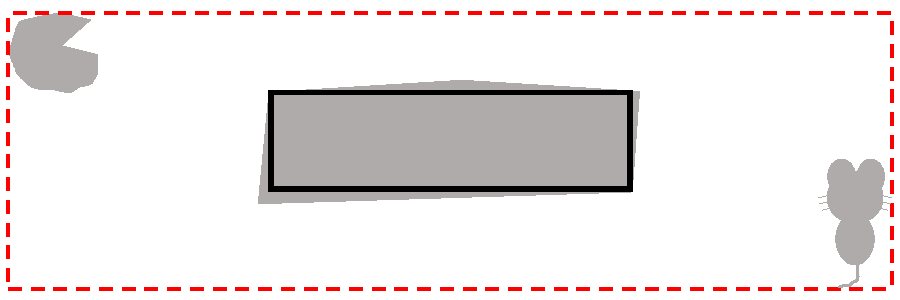
\includegraphics[width=3in]{fig.pdf}
\caption{Example where the underlying distribution $p$ is uniform over the (gray) valid regions. The solid rectangle maximizes our objective since it does not output nonsense (is supported only within the grey matter) and is closest to the $p$ (covers the maximum amount of grey matter). In contrast, the standard maximum likelihood (dashed red) rectangle must fully contain the observed samples, thus generating invalid points most of the time.  }
\end{figure}

Motivated by these observations, we evaluate a generative model $q$ on two axes. First is {\em coverage}, which is related to the probability assigned to future examples drawn from the true distribution $p$. Second is {\em validity}, defined as the probability that random examples generated from $q$ meet some validity requirement. Formally, we measure coverage in terms of a bounded {\em loss}:
$$\Loss(p,q)=\E_{x \sim p}[L(q_x)],$$
where $L:[0,1]\rightarrow [0,M]$ is a bounded decreasing function such as the capped log-loss $L(q_x)=\min(M, \log 1/q_x)$. % or $L(q_x)=\log 1/(q_x+\exp(-M))$. 
A bounded loss has the advantages of being efficiently estimable, and also it enables a model to assign 0 probability to one example (e.g., an outlier or error) if it greatly increases the likelihood of all other data. Validity is defined with respect to a set $V \subseteq X$, and $q(V)$ is the probability that a random example generated from $q$ lies within $V$. 

Clearly, there is a tradeoff between coverage and validity. We first focus on the case of (near) perfect validity. A Valid Generative Modeling (VGM) algorithm if it outputs, for a family of distributions $Q$ over $X$, if it outputs $\hat{q}$ with (nearly) perfect validity and whose loss is nearly as good as the loss of the best valid $q\in Q$. More precisely, $A$ is a VGM learner of $Q$ if for any nonempty valid subset $V \subseteq X$, any probability distribution $p$ over $V$, and any $\eps>0$, $A$ uses $n$ random samples from $p$ and makes $m$ membership oracle calls to $V$ and outputs a distribution $\hat{q}$ such that, $$\Loss(p, \hat{q}) \leq \min_{q \in Q: q(V)=1}\Loss(p,q) + \eps ~\text{ and }~\hat{q}(V)\geq 1-\eps.$$ 
We aim for our learner to be sample and query efficient, requiring that $n$ and $m$ are polynomial in $M, 1/\eps$ and a measure of complexity of our distribution class $Q$.
Furthermore, we would like our algorithms to be computationally efficient, with a runtime polynomial in the size of the data, namely the $n + m$ training examples. 
A more formal description of the problem is available in Section~\ref{sec:problem}.

$A$ is said to be {\em proper} if it always outputs $\hat{q}\in Q$ and {\em improper} otherwise.
In Section~\ref{sec:impossibility}, we first show that efficient proper learning for VGM is impossible. This is an information-theoretic result, meaning that even given infinite runtime and positive samples, one still cannot solve the VGM problem. Interestingly, this is different from binary classification, where it is possible to statistically learn from iid examples without a membership oracle.

Our first main positive result is an efficient (improper) learner for VGM. The algorithm relies on a subroutine that solves the following {\em Generative Modeling with Negatives} (GMN) problem: given sets $X_P, X_N \subset X$ of positive and negative examples, find the probability distribution $q \in Q$ which minimizes $\sum_{x \in X_P} L(q(x))$ subject to the constraint that $q(X_N)=0$. For simplicity, we present our algorithm for the case that the distribution family $Q$ is finite, giving sample and query complexity bounds that are logarithmic in terms of $|Q|$. However, as we show in Section~\ref{sec:infinite-families}, all of our results extend to infinite families $Q$. It follows that if one has a computationally efficient algorithm for the GMN problem for a distribution family $Q$, then our reduction gives a computationally efficient VGM learning algorithm for $Q$.

Our second positive result is an algorithm that minimizes $\Loss(p,q)$ subject to a relaxed validity constraint comparing against the optimal distribution that has validity $q(V)$ at least $1-\alpha$ for some $\alpha>0$. We show in Section~\ref{sec:partial-validity} that even in this more general setting, it is possible to obtain an algorithm that is statistically efficient but may not be computationally efficient. An important open question is whether there exists a computationally efficient algorithm for this problem when given access to an optimization oracle, as was the case for our algorithm for VGM.

\subsection{Related Work}
\cite{KearnsMRRSS94} showed how to learn distributions from positive examples in the realizable setting, i.e., where the true distribution is assumed to belong to the class being learned. In the same sense as their work is similar to PAC learning \citet{Valiant84} of distributions, our work is like agnostic learning \citet{KearnsSS94} in which no assumption on the true distribution is made. 

Generative Adversarial Networks (GANs)~\cite{GoodfellowPMXWOCB14} are an approach for generative modeling from positive examples alone, in which a generative model is trained against a discriminator that aims to distinguish real data from generated data. In some domains, GANs have been shown to outperform other methods at generating realistic-looking examples. Several shortcomings of GANs have been observed \citet{AroraRZ18}, and GANs are still subject to the theoretical limitations we argue are inherent to any model trained without a validity oracle. 

In supervised learning, there is a rich history of learning theory with various types of queries, including membership which are not unlike our (in)validity oracle. Under various assumptions, queries have been shown to facilitate the learning of complex classes such as finite automata \citet{Angluin88} and DNFs \citet{Jackson97}. See the survey of \cite{Angluin92} for further details.  Interestingly, \cite{Feldman09} has shown that for agnostic learning, i.e., without making assumptions on the generating distribution, the addition of membership queries does not enhance what is learnable beyond random examples alone. 
Supervised learning also has a large literature around active learning, showing how the ability to query examples reduces the sample complexity of many algorithms. See the survey of \cite{Hanneke14}. Note that the aim here is typically to save examples and not to expand what is learnable.
 
More sophisticated models, e.g., involving neural networks, can mitigate the invalidity problem as they often generate more realistic natural language and have even been demonstrated to generate \LaTeX{} that nearly compiles \citep{Karpathy15} or nearly valid Wikipedia markdown. However, longer strings generated are unlikely to be valid. For example, \cite{Karpathy15} shows generated markdown which includes:
\begin{quote}
==Access to ''rap===
The current history of the BGA has been [[Vatican Oriolean Diet]], British Armenian, published in 1893.  While actualistic such conditions such as the [[Style Mark Romanians]] are still nearly not the loss.
\end{quote}

Even ignoring the mismatched quotes and equal signs, note that this example has two so-called ``red links'' to two pages that do not exist. Without checking, it was not obvious to us whether or not Wikipedia had pages titled {\em Vatican Oriolean Diet} or {\em Style Mark Romanians}. In some applications, one may or may not want to disallow red links. In the case that they are considered valid, one may seek a full generative model of what might plausibly occur inside of brackets, as the neural network has learned in this case. If they are disallowed, a model might memorize links it has seen but not generate new ones. A validity oracle can help the learner identify what it should avoid generating.

 In practice, \cite{KusnerPH17} discuss how generative models from neural networks (in particular autoencoders) often generate invalid sequences. 
\cite{JanzWPKH18} learn the validity of examples output by a generative model using oracle feedback. 

% !TEX root = Main.tex 
\section{More on the problem formulation in a general 
	adversarial and stochastic settings}
\label{s:set}
%
%We complete the description of the adversarial and stochastic 
%problems initiated in the introduction.    
Let $[a:b]=\{a,a+1,\ldots,b\}$ with
$a,b\in\Integer$, $a\leq b$, and $[a]=[1:a]$.
%For a vector $\w\in \Real^n$, $n\in\Integer$,  $\maxnorm{\w}= \max_{k\in[n]} |\w_k|$. 
A vector indexed by both round $t$ and a specific element
index $k$ is $\w_{k,t}$. We detail the general game protocol in Figure~\ref{fig:protocol}.
%
%
\begin{figure}[H]
\centering
\framebox{
	\begin{minipage}{.95\textwidth}
		\textbf{Input:} the time horizon $\timeHorizon$ and the number of arms $\nArms$\\
		\textbf{For} $t=1,2, \ldots, \timeHorizon$, 
		
$\qquad$\raisebox{.00cm}{\textcolor{bull}{$\blacktriangleright$}}~ simultaneously, the learner chooses arm $\pulledArm_t\in [\nArms]$, and

$\qquad$\raisebox{.00cm}{\textcolor{bull}{$\blacktriangleright$}}~  the adversary picks a gain vector. 
$\gainVector_t\in [0,1]^\nArms$.

$\qquad$\raisebox{.04cm}{\textcolor{bull}{$\blacktriangleright$}}~ Then, the learner 
observes $\gainVector_{t,\pulledArm_t}$.

		After round $\timeHorizon$ is over, the learner 
		recommends the arm  $\recomArm_{\timeHorizon}$ with the objective that $\recomArm_{\timeHorizon} = \bestArm_{\gainVector}$.
	%	\todov{it should be $\recomArm_{n+1}$ ot at least dont say the game stop when $t=n$ be careful with conventions! (starting to change now!)}
	\end{minipage}
}
\caption{General protocol of the adversarial setting. The adversary 
	is oblivious.}\label{fig:protocol}
\end{figure}
%\todomi{may be confusing that adversary observes $\gainVector_{t,\pulledArm_t}$ in General Protocol}
%
\paragraph{Adversarial case} 
      The adversary is denoted as \advPro{}. It is the process that 
     generates $\gainVector$.
     %
   %  In hindsight, at time $t$, %at the end of the game when 
  %   $t=\timeHorizon$, 
    % we can order the arm with respect to their 
     %cumulative gains $\cumulGain_{k}= \sum^{\timeHorizon}_{t=1} \gainVector_{k,t}$. %\todo{X or g?} 
%At the end of the game, $t=\timeHorizon$. 
 Let $(m)$ denote 
the index of the $m$-th best arm in $\setArms$
 and $\cumulGain_{(m)}$ its corresponding 
 cumulative gain
 so that $\cumulGain_{(1)}> \cumulGain_{(2)} \geq \ldots 
 \geq \cumulGain_{(\nArms)}$. Dually to $(\cdot)$, $\langle k \rangle$~denotes 
 the rank of arm $k$ after sorting according to~$\cumulGain_{(\cdot)}$ so that $\langle (k) 
 \rangle=(\langle k \rangle)=k,~ \forall k\in \setArms$.
%\todov{using accolade for the rank is too confusing}
Without loss of generality, note that we assumed there 
exists
 a unique best arm $\bestArm_{\gainVector}=(1)$. %\todov{really no loss of generality?}
%
%\todov{think of how to define here or not \advPro{} }
%
For each arm $k\in \setArms$, we define the gap 
$\gap^\gainVector_k$ as
%
\begin{align*} 
\timeHorizon\gap^\gainVector_{k} \triangleq \begin{cases}  
\cumulGain_{(1)}-\cumulGain_{k} & \text{if } k \neq \bestArm_{\gainVector}, \\
\cumulGain_{(1)}-\cumulGain_{(2)}       & \text{if } k =\bestArm_{\gainVector}.
\end{cases}%\cdot
\end{align*}
%
%\todov{choose how much we want to put that $\gainVector$ as an index everywhere}
The gap can also be written as 
$\timeHorizon\gap^\gainVector_{k} = \big|\max\limits_{i \neq k} 
\cumulGain_{i} - \cumulGain_{k}\big|$. 
%
%
%\todov{call him learner or forecaster?}
%\todov{discuss adaptive or oblivious adversary and think about
% what is the difference for us for the results}
% \todomi{indeed, I think P. Auer makes a distinctions about these}
 $\recomArm_{\timeHorizon} \in \setArms$ is the  arm 
returned by the learner at the end of the exploration phase.  
Given a budget
  $\timeHorizon$ and a fixed adversarial set of rewards 
  $\gainVector$ designed by an  adversary \advPro{}, the
   performance of the learner is measured by the 
   probability
    $\ProErr_{\advPro(\gainVector)}(\timeHorizon)$ 
    of not identifying the best 
    arm, i.e.,~$\ProErr_{\advPro(\gainVector)}(\timeHorizon)
     \triangleq \Pro\left(\recomArm_{\timeHorizon} \neq \bestArm_{\gainVector}\right).$
     The smaller $\ProErr_{\advPro(\gainVector)}(\timeHorizon)$, 
    the better the learner. The probability 
    is taken over the randomness of the learner as $\gainVector$ is fixed.
    An alternative definition of  the best arm, i.e., with
     highest $G_{k}$ in expectation over adversarially 
     sampled $\gainVector$, would lead to an impossible problem. 
     Indeed, it could happen that the best arm in expectation is actually 
     always clearly suboptimal on any realization $\gainVector$.
%
%\todomi{remark: It is somehow uncommon to have $\gainVector$, \emph{sampled} from the adversary..., so  we should comment that it makes sense here.}
%
%
%
%The learner will often chose the arm from a distribution
% at time $t$, $\learnerDist_t$, where $\learnerDist_{k,t}=\Pro(\pulledArm_t=k)$.
%
We define the random variables $\estGainVector_{k,t}$ as
 %
\begin{equation*}
\estGainVector_{k,t} 
\triangleq
 \frac{\gainVector_{k,t}\indicator{\pulledArm_t = k}}
 {\learnerDist_{k,t}}\CommaBin
\end{equation*}
%
for 
arm $k$ at round $t$ and for which  $\Exp_{\pulledArm_t\sim\learnerDist_{t}}
\left[\estGainVector_{k,t}\right]=\gainVector_{k,t}.$
We similarly define $\estCumulGainVector_{k,t} \triangleq \sum_{t'=1}^{t} \estGainVector_{k,t'}.
$
%we have for all $k\in\setArms$,  $\Exp_{\pulledArm_{[t]}\sim\learnerDist_{[t]}}\left[\estCumulGainVector_{k,t}\right]=\cumulGain_{k,t}$.
%\todov{improve the simulation under the expectation}
%
%We say that the adversary is oblivious if $\gainVector_{k,t}$ is independent of $\pulledArm_1,\ldots,\pulledArm_{t-1}$ for all $k\in\setArms$ and $t\in[\timeHorizon]$. Otherwise the adversary is said to be adaptive. 
 %
 %
\paragraph{Stochastic case}
 In stochastic bandits~\citep{Audibert10BA}, that
  we denote \stoPro{}, the distribution~$\nu_{k}$ of arm $k$ is bounded in $[0,1]$ with mean $\mu_{k}$. % and variance $\sigma^2_{k}$. 
 The ordering $(\cdot)$ is such that $\mean_{(1)}>\mean_{(2)}
 \geq\ldots\geq\mean_{(\nArms)}$, as we assume  the uniqueness of the best arm without loss 
 of generality.
 The distributions $\{\nu_{k}\}$ are unknown to the learner.
 %At each round $t$, $\gainVector_{k,t}$ is an independent sample drawn from the 
 %distribution $\nu_{k}$.
% Let $\pullsNumber_{k}(t)$ be the number of times that arm 
% $k$ has been pulled by the end of round $t$.
% %
% Usually the forecaster estimates the expected value of each arm by computing the
% average of the samples observed over time $\widehat{\mu}_{k}(t) = \frac{1}{T_{k}(t)}\sum_{t=1}^{\timeHorizon}\indicator{\pulledArm_t=k}\gainVector_{k,t}$.
 %
 The best arm to be identified is  $\bestArmSto= \argmax_{k\in\setArms} \mean_k$.
 % involved
 % Indeed $\bestArmSto$ is not define for any $\gainVector$ but in expectation with the means. With very high probability (smaller than the probability of errors of interest) the best arms are the same anyway
 %
 Similar to the adversarial case, the gaps are 
 $\gap_{k} \triangleq |\max_{i \neq k} \mean_{i} - \mean_{k}|$, ranked as
$\gap_{(1)} \triangleq \gap_{(2)}\leq\ldots\leq\gap_{(\nArms)}$, 
 and the error 
 %\todom{here the definition of the error included the randomness over rewards as well, right? so maybe not so similar\\
% Victor:
 %That is what i try to explain in the next sentence, that the diff is very small, it is not clear?}
 of the learner is $\ProErr_{\stoPro}(\timeHorizon) 
 \triangleq \Pro\left(\recomArm_n \neq \bestArmSto\right)$.  
 However, unlike in the adversarial case, this definition of the 
 error includes the randomness of rewards.
 Nonetheless, it is only with a probability upper-bounded 
 by $\rho=\cO(\nArms\exp(-\timeHorizon\gap^2_{(1)}))$
   that a $\gainVector\sim\stoPro$ can verify 
   $\bestArmSto\neq\bestArm_\gainVector$. However, this difference 
   with the adversarial formulation is not significant as the 
   probability $\rho$ is never larger than the probabilities of errors studied in this paper 
   and it is often insignificant with 
   respect to it.
 
\paragraph{Notions of complexity} Given 
gaps $\gap_{k}$ for $k\in\setArms$, we define two notions of 
complexity of the identification task, 
$\complexitySR$ and $\complexityUnif$, that were introduced by~\cite{Audibert10BA}. 
% In the stochastic case, these notions are defined 
In particular,
 %
 \[
 \complexitySR
 \triangleq
 \max_{k\in\setArms}\frac{k}{\gap^2_{(k)}}
 \qquad\text{and}\qquad
 \complexityUnif 
\triangleq
% \nArms\max_{k\in\setArms}\frac{1}{\gap_{(k)}^2}=\frac{\nArms}{\min_{k\in\setArms}\gap_{(k)}^2}
% ~=~
% \nArms\max_{k\in\setArms}\frac{1}{\gap_{(k)}^2}
% =
 \frac{\nArms}{\gap_{(1)}^2}\cdot
 \]
  %\todov{which way to write tit? }
  %
  %\todomi{isn't this a good place to relate to the complexities in the prior papers?\\
 % Victor: These are the complexity of previous paper}
   $\complexitySR$ relates to the complexity of the stochastic 
   case. $\complexityUnif$ will be used both in the 
   adversarial and stochastic cases. 
In the adversarial case, the complexity and the gaps 
are defined with respect to $\gainVector$ and 
but we also sometimes  write the uniform complexity as  $ \complexityUnif (\gainVector)$ for clarity.


\paragraph{Class of problems}  We define a set of classes to group problems with
very similar gap structure and with complexities that are only a 
constant multiplicative factor apart.
For any $0<\gap_1=\gap_2\leq\gap_3\leq \ldots\leq 
\gap_\nArms\leq 1/8$, we define a \textit{problem class} 
$\Gaps_{c}$ with
$c\geq 1$. 
Given these gaps and $c$, in the adversarial case, we say that 
$\gainVector\in\Gaps_{c}$  if  for all $k\in\setArms$, $\gap_k/c
 \leq\gap^{\gainVector}_k\leq c\gap_k$ except for only one 
 arm~$\refarm$  whose gap is related to the smallest gap as $\gap_{1}/c\leq\gap^{\gainVector}_{\refarm}\leq c\gap_{1}$.
In the stochastic case, $\stoPro\in\Gaps_{c}$ under 
the same condition on its gaps defined as $\gap_{k} \triangleq
 |\max_{i \neq k} \mean_{i} - \mean_{k}|$  for $k\in\setArms$. 


%Our results will expressed in a
%context where \advPro{} generates deterministically
%$\gainVector$ before the start of the game and therefore 
%in that case \advPro{} and $\gainVector$ are essentially 
%the same thing.
%However in some proofs we will construct adversaries \advPro{} that generate 
%randomly  $\gainVector$ before the game starts. In those cases we will be more 
%careful to discriminate  between $\gainVector$ and \advPro{} 
%in the notations.


%\section{Notation and technical results for the proofs}
%\todov{unused at the moment}
%Following the notations in\cite{Carpentier16TB}:
%
%For two distributions $\nu$, $\nu'$ defined on $\Reals$ and that are such that $\nu$ is absolutely continuous with
%respect to $\nu'$, we write
%\[
%KL(\nu,\nu')
%~=~
%\int_{\Reals}\log\left(\frac{d\nu(x)}{d\nu'(x)}\right)d\nu(x)
%\]
%for the Kullback Leibler divergence between distribution $\nu$ and $\nu'$.

% !TEX root = Main.tex
\section{General adversarial case: An optimal 
	learner can play uniformly at random}
\label{s:ULGenAd}
%
In this section, we define a simple learner  (\RULE{}) and in Theorem~\ref{th:UPARU}, we 
provide an upper bound on its probability of error 
 depending on the gap in hindsight. 
We also give  a matching lower bound for the general 
adversarial best-arm identification (Theorem~\ref{th:LOWadPRO}) 
proving that \RULE{} obtains the optimal gap-dependent rates of error against worst-case adversaries.
%
%\begin{figure}
%    \centering
%    \framebox{
%        \begin{minipage}{.85\textwidth}
%            \textbf{Given:} $K$ \\
%            For $t=1,2, \ldots, \timeHorizon$\\
% \textcolor{white}{erere}Select arm $\pulledArm_t\in [\nArms]$ 
% with probability $\learnerDist_{k,t}=\Pro(\pulledArm_t=k)
% =\frac{1}{\nArms}$ for all $k\in\setArms$.
%
%            \textbf{Returns:} $\recomArm_\timeHorizon=\argmax_{k\in\setArms} \estCumulGainVector_{k,\timeHorizon}$ 
%        \end{minipage}%\todov{inclue pt in this def?}
%    }
%    \caption{The \emph{Random Uniform Learner (\RULE{})} }\label{fig:uniform}
%\end{figure}
%

%The \emph{Random uniform  learner} (\RULE{}) is detailed in 
%Figure~\ref{fig:uniform}. 
%\todov{if in need for space, we can remove the figure to explain a uniform sampling!}
%Select arm $\pulledArm_t\in [\nArms]$ 
% with probability $\learnerDist_{k,t}=\Pro(\pulledArm_t=k)
% =\frac{1}{\nArms}$ for all $k\in\setArms$
At round $t$, the \emph{random uniform  learner} (\RULE{}) 
selects an arm $\pulledArm_t\in [\nArms]$ uniformly at random, i.e., 
with probability $\learnerDist_{k,t}\triangleq\Pro(\pulledArm_t=k)
\triangleq 1/\nArms$ for all $k\in\setArms$.
%he choice of $\pulledArm_t$ is made uniformly  at 
%random from $\setArms$.
At the end of the game, the recommended 
arm $\recomArm_\timeHorizon$ is the one with highest 
estimated  
%\todom{estimator is unbiased but here we have an actual realization that is biased\\
%Victor: What do you mean biased? the realisation is what it is.} 
cumulative gain, 
$\recomArm_\timeHorizon \triangleq \argmax_{k\in\setArms}
\estCumulGainVector_{k,n}$. 
%We first prove an upper bound on the probability of error of ARU.
%
\begin{restatable}[\textcolor{titleTh}{Upper bound for \RULE{} in the adversarial case}]{theorem}{tata}\label{th:UPARU}
	For any horizon $\timeHorizon$, given rewards $\gainVector$ 
	chosen by an oblivious adversary, with $\gainVector_{k,t}\in [0,1]$ 
	for all $t\in[\timeHorizon]$ and for all $k\in\setArms$, \RULE{}  
	outputs an arm $\recomArm_\timeHorizon$
	with the guarantee that its probability of error 
	$\ProErr_{\advPro(\gainVector)}(\timeHorizon)$ verifies    
	%
	%    \todov{is that true against an adaptive adversary be precise}
	\[
	%\mathbb{P}\big[\recomArm_\timeHorizon \neq \bestArmAd\big] 
	\ProErr_{\advPro(\gainVector)}(\timeHorizon)
	\leq
	\nArms\exp\left(-\frac{3\timeHorizon}{28\complexityUnif(\gainVector)}\right)\!\cdot
	\]
	%    
	%Note that the factor $\nArms$ in front of the exponential is easily replaced by a $\log\nArms$ using a decomposition of the error into groups of halves as in \cite{Karnin13AO}. \todov{should we mention that? should actually get the log from the proof?}
\end{restatable}
%\todov{maybe define $\mean_{k,t}$,$\gap_{k,t}$, is this needed?}
%\todov{should we have $\gainVector$ here in the equation?}
%
%\todov{should be able to remove the factor 2 because it appears i think if you use the two-sided Bernstein inequality... and we might only need one side}

\noindent\textbf{Sketch of the proof} \textit{(full proof in 
	Appendix~\ref{app:proofupadPRO})}:
The deviation of 
$\estCumulGainVector_{k,t}$ from $\cumulGain_{k,t}$ is bounded by 
a Bernstein bound which applies  since, given 
$\gainVector$ and the fact that $\learnerDist_t$ is fixed to 
constant values for all the rounds, the $\estGainVector_{k,t}$ 
are independent.  $\estGainVector_{k,t}$ are scaled 
Bernoulli random variables where the use of the Bernstein 
bound leads to a bound that scales with the 
variance of the $\estGainVector_{k,t}$ which is $\nArms$. Using a  Hoeffding bound would lead to  a 
bound that scales with the range of the $\estGainVector_{k,t}$ \emph{squared}
which is $\nArms^2$. %The final bound is obtained by a union argument is over all the different arms.
%
%\todomi{did we check that all these assumptions BELOW are compatible?\\
%Victor: Why would they?
%the gaps are arbitrary: no assumption. Then K is large. then you set n large enough so that the condition is valid \\
%M: is there is at least one combination of parameters when $K\ge 4095$ and ...
%}
\begin{restatable}[\textcolor{titleTh}{Lower bound for the adversarial problem}]{theorem}{toto}\label{th:LOWadPRO}
	Given any problem class $\Gaps_{3}$ with associated complexity
	$\complexityUnif$,    
	for any learner, for any horizon $\timeHorizon$ such that    
	$\nArms\exp\left( -\timeHorizon\gap^2_1 /128\right)\leq 1/128$ and $\nArms\geq 4096$, there exist 
	$\gainVector^1\in\Gaps_{3}$ and $\gainVector^2\in\Gaps_{3}$ so that  
	the  probabilities of error suffered by the learner on 
	$\gainVector^1$ and $\gainVector^2$, denoted $\ProErr_{\gainVector^1}(n)$ 
	and  $\ProErr_{\gainVector^2}(n)$ respectively, verify
	%
	\[
	%
	\max\left(\ProErr_{\gainVector^1}(n),\ProErr_{\gainVector^2}(n)\right)
	%
	\geq
	%
	\min\left(
	\frac{1}{128}\exp\left(-\frac{32\timeHorizon}{\complexityUnif}\right)\CommaBin
	\frac{1}{32}
	\right)\!\cdot
	%
	\]     
	%
\end{restatable}
%
\noindent\textbf{Sketch of the proof} \textit{(full proof given 
	in Section~\ref{app:prooflowadPRO})}:
We construct two similar bandit problems. Between the two 
problems, only one arm differs by a change in the mean of 
order $\gap_{(1)}$ for about $\timeHorizon/(2\nArms)$ 
time steps. Therefore, using a change-of-measure argument, 
with a probability of order $\exp(-\timeHorizon/\complexityUnif)$ these two problems generate each a 
set of rewards,  $\gainVector^1$ and 
$\gainVector^2$ respectively, that the learner is not able to 
discriminate. In this undecidable case,  the learner 
still needs to recommend an estimated best arm.
However, these two problems have different best arms 
$\bestArm_{\gainVector^1}\neq\bestArm_{\gainVector^2}.$ 
Therefore, the learner makes a mistake of order 
$\exp(-\timeHorizon/\complexityUnif)$ on 
at least one of the two problems.

We consider any \emph{fixed} learner and let us have $K$ base Bernoulli distributions with  
means $\mean_1 \triangleq 1/2$ and for all $k\in[2:\nArms], \mean_k=1/2-\gap_k$. 
We consider the first half of the game from round $t=1$ 
to a round 
$\lfloor n/2\rfloor$ as a  set of rounds denoted 
$\earlyPhase$. 
%Because the total number of pulls by the learner is 
%limited by $\lfloor n/2\rfloor$ 
%in $\earlyPhase$, 
By Dirichlet's box principle, 
there exists at least one  arm, denoted $\refarm$,
that is pulled less than $\cO(\timeHorizon/(2\nArms))$ in 
expectation during $\earlyPhase$. This arm, that the learner 
does not explore very much, is then used to 
construct the two bandit problems that look similar to the learner. 
We now describe the two problems in detail.
%and therefore difficult 
% from the original Bernoulli distributions.
%The two bandit problems sample randomly their set of rewards $\gainVector$. 

The first problem  is  following the 
original Bernoulli distributions for all arms in phase~$\earlyPhase$.
Then the second part of the game, $t=\lfloor n/2\rfloor+1,
\ldots,\timeHorizon$, is deterministic.  Almost all the 
rewards of all the arms are $0$, except some rewards of 
$\refarm$ which are set to $1$. This is done so that in 
expectation in this setup, the total reward of $\refarm$ 
is $\timeHorizon(1/2-\gap_1)$ and therefore it becomes the second
best arm. %\todov{make it more readable}

The second problem only differs from the previous one 
in its first, stochastic  part and only affects~$\refarm$ which instead of 
having the Bernoulli mean $1/2-\gap_{\refarm}$,  has now 
a mean 
of $1/2-\gap_{\refarm}+2\gap_{1}$. In this problem, 
the effect of the deterministic part is that in the end, 
when $t=\timeHorizon$, the expected mean of  arm 
$\refarm$ is 
$(1/2+\gap_1)$ instead of $(1/2-\gap_1)$, therefore in this case, 
$\refarm$ becomes the best arm.
%
%The two problems will be hard to discriminate for the learner but he will have to make a different choice in both. the event on which the learner will be confused with have a probability of order $\exp\left(-\frac{\timeHorizon}{\complexityUnif}\right)$ hence the lower bound.
%
% i think the improvement would be from $1/\nArms\exp()$ to $\exp()$.
\begin{remark}
	The assumption $\nArms\exp(-\gap^2_{(1)}
	\timeHorizon/8)\leq 1/32$ is mild. 
	Essentially, it  asks for horizon $\timeHorizon$ to be 
	large 
	enough so that the stochastic problem is learnable within 
	$\timeHorizon$ rounds. The assumption on~$\nArms$ is 
	likely to be an artifact of the proof. Even with this 
	assumption, our main message holds, in general, 
	no learner can perform better than the random uniform leaner, up to constants.
\end{remark}%
% !TEX root = Main.tex
%
\section{The best of both worlds challenge}
\label{s:FormuBOB}
%
In this section, we ask if we can have a learner 
that performs optimally under adversarial and stochastic rewards. 
The lower bound in Theorem~\ref{th:lowBOB} shows that in general,
this is impossible.\vspace{.2cm}

%First we recall the stochastic problem and introduce its notations.

%therefore this not a very interesting problem in the sense that no smart thing can be done in the worst case. So why not having an algo that still possess this worst case guaranty like uniform but also has a nice behaviour on easier data such as, as a start, the stochastic case and perform there as good as SR.
%
\paragraph{Existing robust solutions?} In the stochastic setting,
a state-of-the-art algorithm, Sequential Halving (\SH{}, 
\citealp{Karnin13AO})---see also Successive Rejects (\SR{}) 
by~\cite{Audibert10BA})---guarantees 
$\ProErr_{\stoPro}(\timeHorizon) \leq \cO\left(\log\nArms\exp
\left(-\timeHorizon/(\complexitySR\log\nArms)\right)\right)$. 
However, as discussed in the introduction, \SR{} or \SH{} can fail  
against a worst-case adversary.
On the other hand, as discussed by~\cite{Audibert10BA},  
uniform-like algorithms (like \RULE{}) can only guarantee that
in the stochastic case, we get $\ProErr_{\stoPro}(\timeHorizon) \leq  
\tcO\left(\exp\left(-\timeHorizon/\complexityUnif\right)\right)$.
In general, $\complexitySR\leq\complexityUnif$ and 
in some problems, we even have $\complexitySR=\complexityUnif/\nArms$. 
Therefore, \SH{} can notably outperform uniform 
algorithms in the stochastic case.%\vspace{.2cm}

%Un

%So the stochastic environment is already solved (reference the literature). State of the art algorithm are of the successive regret, SR, family. More over the uniform type algorithm are shown to be sub-optimal.
%As discussed somewhere (\todo{not done yet} not done yet! put it here or in the previous section? ) we have that SR is easily beaten in the adversarial setting.
%So we can notice that the algorithms that are optimal in one setting are suboptimal in the other. This raise a question:
%But what about solving it and 
%being as good as uniform against adversaries. can we have best of both worlds. 
%we think no and we first provide a lower bound.
%
\paragraph{The best of both worlds} We now reveal the holy grail of our endeavor, which is the following question: Does there exist 
a learner, unaware of the nature of the reward-generating process, that guarantees for any  $\timeHorizon$, for any stochastic problem 
\stoPro{}, and any set of rewards~$\gainVector$ that 
 its respective probabilities 
of misidentification $\ProErr_{\stoPro}(\timeHorizon) $ and
$\ProErr_{\advPro(\gainVector)}(\timeHorizon) $ simultaneously verify 
%for any iid problem and adversarial $\gainVector$,
%\todomi{in sto and adv, the expectation is taken (maybe) over different things. Is this not a problem when we compare them to each other?}
\[
\ProErr_{\stoPro}(\timeHorizon) 
\leq
\tcO\left(\exp\left(-\frac{\timeHorizon}{\complexitySR\log\nArms}\right)\right)
\text{ ~~~and~~~ }
\ProErr_{\advPro(\gainVector)}(\timeHorizon) 
\leq  
\tcO
\left(\exp\left(-\frac{\timeHorizon}{\complexityUnif(\gainVector)}\right)\right)\textbf{?}
\]
%where $c_\nArms$ and $c'_\nArms$ are quantiti
%
\paragraph{Why is the BOB question challenging?}
The learner could choose, 
for arm $k$, at round $t$, to use the 
cumulative gain  estimator  $\estBiasCumulGain_{k,t} = 
\frac{t\sum_{t'=1}^{t}\indicator{\pulledArm_{t'}=k}\gainVector_{k,t'}}{\sum_{t'=1}^{t}\indicator{\pulledArm_{t'}=k}} 
$.
This estimator can be potentially highly biased if it is used against a 
malignant adversary. For this reason, we base our approach on 
the estimator $\estCumulGainVector_{k,t} = \sum_{t'=1}^{t}
\frac{\gainVector_{k,t'}}{\learnerDist_{k,t'}}\indicator{\pulledArm_{t'} = k}$.
However, this usage potentially introduces high variance in our estimates;
the final amount of variance of $\estCumulGainVector_{k,n}$ 
is the sum of the variance of each~$\estGainVector_{k,t}$ and 
therefore scales with $\sum_{t'=1}^{t} 1/ \learnerDist_{k,t'}$.
% scaling with $\sum_{t'=1}^{t}\frac{1}{\learnerDist_{k,t'}}$.
The high variance is most damaging in the stochastic case when trying 
to have a learner based on $\estCumulGainVector_{k,t}$ to obtain the 
optimal error rates of \cite{Karnin13AO}. Indeed, these 
optimal rates are obtained by algorithms using 
$\estBiasCumulGain_{k,t}$, which has no bias and small 
variance in the stochastic case.
Therefore,  
we strive to characterize the minimum amount of 
unavoidable variance of the mean estimators of each arm.
%As a consequence,  we are capturing the power of the adversary to fool the 
%learner.
%This is especially critical in the stochastic case where the learner is trying to obtain an error rate comparable to the one of the stochastic state-of-the-art algorithm that are usually  using $\estBiasCumulGain_{k,t}$ in a safe
%If the arms are pulled uniformly, the variance is of order $K$, 
%which is very large.
The learner would like to allocate more pulls at any round $t$ 
to the arms that are among the best arms, which means having large 
$\learnerDist_{k,t}$ for these arms. Indeed,  discriminating 
between them is the hardest part of the task and large 
$\learnerDist_{k,t}$ reduces the variance term $1/\learnerDist_{k,t}$. 
%However pulling more the best arm especially difficult for the 
%  Moreover, because of our use of $\estCumulGainVector_{k,t}$, the learner should try to pull more the best
%  arms  as early in the game as possible %\todom{not sure, this  statements depends on how $1/\learnerDist_{k,t}$ depends on $t$}
%   to reduce, for small $t$, the variance term $1/\learnerDist_{k,t}$.
%But pulling more the best arms is exactly the problem the 
%learner is already trying to solve.
However, it is natural to 
think that the learner is not able to guarantee that it pulls 
the best arms at the beginning of the game more than in a 
uniform fashion.
If the arms are pulled uniformly, the variance is of order $K$, 
which is very large.
The amount of time that the learner accumulates large variance on its estimate of the best arms because they are not yet well identified  determines the final probability of error. 
Intuitively, the lower bound in Theorem~\ref{th:lowBOB} 
constructs worst-case examples 
showing that any learner cannot pull the best arm more than 
a certain amount in some period of the game because it is difficult to identify the best arms. 
Therefore, 
this learner is susceptible to be tricked by an adversary. Our new learner
in Section~\ref{s:UpperBOB} tries to limit this effect by 
making early and almost costless bets on what are the 
best arms given the early rewards and starts to pull them more right away.
Note that if any learner allocates pulls uniformly for the first half of 
as it is 
done in  algorithms like \SR{} or \SH{}, %~\citep{Audibert10BA}, 
then even if the pulls are randomized,
the variance of the  
estimator  $\estBiasCumulGain_{k}$ of  arm $k$ would still scale with $\nArms$ which prevents 
outperforming even the static random uniform learner.

Another approach could be a learner that determines online 
if the observed rewards are stochastic. This was used by~\cite{Bubeck12BB} and~\cite{Auer16AA}. They 
detect if the difference between $\estBiasCumulGain_{k,t}$
and $\estCumulGainVector_{k,t}$
is way too large. However, their bound itself uses  terms 
depending
on $\nArms$ and the variance of each arm, 
$1/\learnerDist_{k,t}$, which leads to similar open questions 
as discussed just above. In this paper, inspired by the approach 
of~\cite{Seldin14OP},  we give a practical 
simple parameter-free and versatile algorithm.  Furthermore,  the algorithms
that are based on stochastic tests are usually cumbersome and complex,  as discussed by~\citealp{Seldin14OP}.
% !TEX root = Main.tex
%
%\subsection{Lower Bound for the Stochastic \& Adversarial Rewards}
%\label{s:LowBOB}
\paragraph{Why is the best of both worlds unachievable?}
% 
We define a new notion of complexity, $\complexityBoth$ as
%
\[
%
\complexityBoth 
\triangleq
\frac{1}{
\gap_{(1)}}
\max_{k\in\setArms}\frac{k}{\gap_{(k)}}\cdot
%
\]
%
$\complexityBoth $ is a complexity for
the stochastic case.
As we detail  in Remark~\ref{rem:LOWbobCOMP}, 
$	\complexitySR\leq\complexityBoth\leq\complexityUnif.$
%Let $\mathcal S$ be the set of stochastic problem such that
%The upcoming Theorem~\ref{th:lowBOB} shows that
%for any $\nArms$ specified gaps, $0<\gap_1=\gap_2\leq\gap_3\leq \ldots\leq \gap_\nArms\leq 1/8$, 
%a stochastic problem can be built with a very similar gap landscape 
%and a complexity changed by at most a factor of $2$ such that on this problem
% it is not possible to have a probability of error 
%smaller than 
%$	\frac{1}{64}\exp\left(-512\frac{\timeHorizon}{\complexityBoth}\right)$
% %on any stochastic problem
%  without  having 
%  a probability of error  not converging to $0$ with large $\timeHorizon$
%   on some adversarial problem with
%  again a similar gap landscape.
%
\begin{restatable}[\textcolor{titleTh}{Lower bound for the BOB challenge}]{theorem}{thi}\label{th:lowBOB}
     For any class problem $\Gaps_{4}$, for any learner, 
     there exists an i.i.d.\,stochastic problem $\stoPro\in\Gaps_{4}$ with complexity $\complexityBoth$,
     such that  for any~$\timeHorizon$ satisfying  	$\nArms\exp\left(-\gap^2_1\timeHorizon\right/32)\leq 1/32$,  if
	the probability of error of the learner
	 on  \stoPro{}   
	satisfies
%	
	\[	
\ProErr_{\stoPro}(\timeHorizon)
	\leq
	\frac{1}{64}\exp\left(-\frac{2048\timeHorizon}{\complexityBoth}\right)\!\CommaBin
	\]	
%
	then there exists an adversarial problem $\gainVector\in\Gaps_{4}$
	   that  makes the learner suffer a 
	constant error,
	%
	\[	
	\ProErr_{\advPro(\gainVector)}(\timeHorizon)
	\geq
	 \frac{1}{16}\cdot
	\]
	%
      \end{restatable}    
%
\begin{remark}\label{rem:LOWbobCOMP}
	In general, we have
	%
	\[
	\complexitySR\leq\complexityBoth\leq\complexityUnif.
	\]
	%
%We first compare the complexities in a general regime. Then we spell out three different regimes to intuitively explore when the inequalities in the previous equation are strict or not.
Below, we compare the three  complexities in 
three specific gap regimes in order to intuitively explore   whether
the inequalities in the previous equation are strict or not. 
Interestingly, while in two regimes  $\complexitySR=\complexityBoth$, in the third regime, called the `square-root gaps', we can obtain $\complexityBoth=\sqrt{\nArms/2}\complexitySR$.  
This equality shows that on some problems and for large values of $\nArms$,
% 	\todovout{actually really large value on K , like millions !!! :(, i am not sure we want to comment on that no?those numerical constants!}
 our lower bound on 
the complexity of the BOB problem is 
significantly larger than the complexity of the strictly stochastic case.
This ultimately shows that no  learner can guarantee the BOB in general   and that any learner  that is optimal in all strict stochastic problems is then inconsistent against
worst-case adversaries.
	\end{remark}
%\begin{description}
%	\item[General Regime:] Let the set $S$ of pairs $(k,\alpha)$, be $S=\{k\in\setArmsmo,\alpha\geq 0 : \gap^{\alpha}_{(1)}=\frac{\gap^{\alpha}_{(k)}}{k}\}$. This set is not empty as for each $k$ it contains the pair $\left(k,\alpha=\frac{\log k}{\log\left(\frac{\gap{(k)}}{\gap_{(1)}}\right)}\right)$
%	Let us denote $\kappa=\max_{k,\alpha\in S} k^{\frac{1}{\alpha}}$
	%
	\paragraph{\raisebox{.04cm}{\textcolor{bull}{$\blacktriangleright$}}~Flat regime}  We assume all the gaps are equal, 
$k\in\setArms,~ \gap_k=\gap_{1}$. Then, 
$\complexitySR=\complexityBoth=\complexityUnif$. Having $\complexitySR=\complexityBoth$  shows that our  
stochastic BOB lower bound for robust learners (Theorem~\ref{th:lowBOB}) using $\complexityBoth$ is of the same order as the one in the 
strict stochastic setting~\citep{Audibert10BA} using $\complexitySR$.   
In this stochastic regime, \RULE{} is optimal while being robust to an adversary.
%
\paragraph{\raisebox{.04cm}{\textcolor{bull}{$\blacktriangleright$}}~Super-linear gaps} Let $(2)\in\argmin_{k\in\setArms} (\gap_{(k)}/k).$ 
This holds if 
$\forall k\in[3:\nArms],$ we have that $\gap_{(k)}=k\gap_{(1)}$, $\gap_{(1)}\leq 1/\nArms$. Then, 
$\complexitySR=\complexityBoth=(2/\nArms) \complexityUnif$. 
Again, our BOB lower bound is of the same order as in 
the strict stochastic setting. This seems to indicate that in this case, BOB is achievable. However, it is not achieved by the uniform 
learner that is clearly suboptimal. This observation demands a new robust learner. Intuitively,  the learner can  
identify bad arms quickly
and  start focusing early on the best arms without incurring 
high variance on its estimates for them.
%
%\todov{think more about the right 2s!}
\paragraph{\raisebox{.04cm}{\textcolor{bull}{$\blacktriangleright$}}~Square-root gaps}   We assume $(2)\!\in\!\argmin_{k\in\setArms} (\gap^2_{(k)}/k).$ 
%This means that for all $k\in\setArms$, $\gap_{(1)}\leq \frac{\gap{(k)}}{\sqrt{k}}$. 
Let us denote arm $j$ for which  $j\in\argmin_{k\in\setArms} (\gap_{(k)}/k)$. 
For some constant $c$, let $\gap_{(1)}=c\gap_{(j)}/j$. We have 
$c\leq \sqrt{2j}$ because  $\gap^2_{(1)}/2 \leq \gap^2_{(j)}/j$ 
as  $(2)\in\argmin_{k\in\setArms} (\gap^2_{(k)}/k)$.
Therefore,  \[\complexitySR=\frac{2}{\gap^2_{(2)}}=\frac{2}{\gap^2_{(1)}}= \frac{2}{\gap_{(1)}} \frac{j}{c\gap_{(j)}}=\frac{2\complexityBoth}{c}=\frac{2\complexityUnif}{\nArms}\cdot\]	
We can get $c=\sqrt{2j}=\sqrt{2\nArms}$.
This happens if 
$\sqrt{\nArms/2}\gap_{(1)}=\gap_{(\nArms)}$ and
$\sqrt{k/2}\gap_{(1)}\geq\gap_{(k)}$ for $k\in[3:\nArms-1]$. 
Then,  we get  $\sqrt{\nArms/2}\complexitySR=\complexityBoth$.
$\complexityBoth$ is $\sqrt{\nArms/2}$ larger than the complexity of
the strictly stochastic setting.
Intuitively,  the learner needs to spend some time to 
identify the `square-root gaps' suboptimal arms before starting 
to focus on the best arms. This makes it suffer an additional amount
of variance on its estimates for the best arms.
%\vspace{.1cm}
%
%\textbullet~ If all the gaps are such that for all $i$ , $\gap_i/i$ are
% equal (or more generally if, which means
% $\gap_1$ is quite small comparatively to the other gaps, the gaps in the example are increasing rapidly : linearly), we have the lowerbound 
%  $\complexitySR=\complexityBoth=\frac{1}{\nArms}\complexityUnif	$
%   the normal lowerbound again
%
%\textbullet~ If all the gaps are such that for all $i$ , $\gap^2_i/i$ are
% equal (or, more generally, If $1=\argmin_k \gap^2_k/k$, which 
% means arm 1 is quite small comparatively but as small as in
%  the previous case!, the gaps are increasing in a square root fashion ), in this case we have  $K=\argmin_k \gap_k/k$ we have the lowerbound 
%  $\complexitySR=\frac{1}{\sqrt{\nArms}}\complexityBoth=\frac{1}{\nArms}\complexityUnif	$ 
%  which is a new lowerbound larger than in the traditional case so 
%  thats cool. Indeed note that this is a case where the definition of the 
%  classical complexity is $\exp(-N\gap^2_1)$
%  
%  \todovout{\textbullet~ Think about other examples, what can we say in general? We can add something bout general geometric setting where all $\frac{i}{\gap^\alpha_i}$ are the same.}

%
%\begin{remark}
%The assumption $\nArms\exp\left(-\frac{1}{32}\gap^2_{(1)}\timeHorizon\right)\leq 1/32$ is mild. 
%Essentially, at most, it  asks for $\timeHorizon$ to be large 
%enough so that the stochastic problem is solvable within the budget $\timeHorizon$.
%% $\timeHorizon$ is required to be large enough here.
%\end{remark}%
%

\vspace{.5cm}
\noindent\textbf{Sketch of the proof} 
\textit{(full proof in 
	Appendix~\ref{app:prooflowBOB})}:
Our proof of the lower bound uses some arguments of purely stochastic best-arm identification 
lower bounds of~\cite{Audibert10BA} and~\cite{Carpentier16TB}.
We have been also inspired by the lower bound of~\cite{Auer16AA} 
for the BOB question for the cumulative regret. However, 
our specific construction is new.
%\todov{thats a long sketch! should we shortening it or remove it? or no}

Consider a fixed learner. 
%To maximize 
%the bound we will set $i=\argmax_{k\in\setArmsmo} \frac{k}{\gap_{k}}\cdot$
%Let $n_i=n\dividefac_i$, with $\dividefac_i=\gap_1/\gap_i\leq 1$ be a number of early rounds in the game.
%\todov{woops do we have an extra condition here!?}
%As in the proof of Theorem~\ref{th:LOWadPRO} discussed in 
%Section~\ref{s:ULGenAd}, 
%We construct two similar bandit 
%problems, one stochastic and one adversarial.
We construct a stochastic and an adversarial problem.
Between the two problems, only one arm differs.
% by a change in the mean 
%of order $\gap_{i}$. Also this arm that will be observed by the learner only $\timeHorizon_i/i$ times. 
We bound the number of pulls from the learner on this arm.
Using a change-of-measure argument,  
 with a probability  $\cO\left(\exp\left(-\timeHorizon/\complexityBoth\right)\right)$ 
 the two problems are impossible to discriminate. 
However, the two problems have different best arms. 
Therefore the learner makes a mistake $\cO\left(\exp\left(-\timeHorizon/\complexityBoth\right)\right)$ 
on at least one of the two problems.

Let us define $K$ base Bernoulli distributions with  
means $\mean_1 \triangleq 1/2$ and for all remaining $k\in[2:\nArms], \mean_k\triangleq/2-\gap_k$. 
 % that we call $\earlyPhase_i$.
Let $i\in\setArmsmo$ be  an arbitrary arm.
Let $n_i\triangleq n\dividefac_i$, where $\dividefac_i \triangleq \gap_1/\gap_i\leq 1$, is a number of early rounds in the game.
Because the total number of pulls by the learner is 
limited by $\timeHorizon_i$ 
during this phase, by Dirichlet's box principle,  there exists at least $K-i+1$  arms included in $[2:\nArms]$ %$\{(2),\ldots,(\nArms)\}$.
that are pulled  by the learner less than $\cO(\timeHorizon_i/i)$ times in 
expectation. 
Therefore, in this set of arms,  there is an arm, 
%($\refarm=1$ by construction),
 denoted $\refarm$, that 
 has a gap of order or smaller than $\gap_{i}$.
 This arm, with a small gap, that the learner does 
 not explore very much, is then used 
 to  construct the two similar bandit problems 
 that the learner has a hard time to differentiate.
%
The stochastic problem is made by only modifying the
original Bernoulli distribution of arm $\refarm$  
by setting it  to 
$\mu_{\refarm} \triangleq 1/2 + \gap_1/2$. 
The adversarial problem samples  $\gainVector$ randomly: 
 It is mimicking the stochastic 
problem  for all rounds and all arms with the exception 
of the $\refarm$ during the first  $\timeHorizon_i$ 
rounds of the game where the gains are from 
the base Bernoulli distribution (with mean $1-\gap_{\refarm}$).
%distributions until the end of phase $A_i$ and then switch to the same distributions as problem 1.




If  $\dividefac_i\geq \gap_1/\gap_i$--- 
fixing a large enough phase at the beginning to 
modify the identity of the best arm---then  the best 
arms in both problems are different. The event on which the 
two problems are impossible to discriminate has a probability of~$\cO\left(\exp(-\timeHorizon_i(\gap_i)^2/i\right)$. %\leq\exp(-\timeHorizon_ia_i\gap^2_1/i)\right)$.
To maximize this probability, we minimize $\dividefac_i$ 
while still ensuring  to  have the change of best arm 
between the two problems, by setting $\dividefac_i  \triangleq\gap_1/\gap_i$.
Therefore, the probability is now   
$\cO\left(\exp(-\timeHorizon\gap_{1}\gap_i/i)\right)$.
Again to maximize  it, we choose 
$i \triangleq \argmin_k (\gap_k/k)$ and obtain the claimed result for some fixed $\gainVector$.
%
%
% !TEX root = Main.tex
\section{A simple robust parameter-free algorithm for stochastic \& adversarial rewards}
\label{s:UpperBOB}
%
In this section, we present a new learner 
and analyze its theoretical performance against any i.i.d.\, stochastic 
problem or any adversarially designed rewards.

We call the algorithm \ProbabilityONE{}, denote it by \Pone{}, %\todovout{is this english?, 'denote it'?},
and detail it in Figure~\ref{fig:probaoneAlgo}.
Intuitively,  \Pone{} pulls the estimated best arm with 
``probability'' one, the estimated second best arm with ``probability'' 
one half, the estimated third best arm with ``probability'' one 
third, and so on until pulling the estimated worst arm with ``probability'' one over $\nArms$.\textsuperscript{\ref{foot:break}} 
In order to get proper probabilities, we need to normalize  
them by the $\nArms$-th harmonic number %$\bar\log(\nArms)$ where %\todo{the algorithm could be defined so that the two best arm are pulled equally to make a bit more sense but I guess it doesn't really matter}
$\bar\log \nArms =\sum_{k=1}^\nArms (1/k)$, where $\bar\log \nArms\leq \log\nArms+1$ for all positive integers $\nArms$.
% \todov{the relation between $\bar\log(\nArms)$ and $\log(\nArms)$ should be written somewhere}
% \todovout{michal, no? figure[H] for this algo? :) MV: like this?}
\begin{figure}[H]
	\centering
	\framebox{
		~~~~~~~~~    \begin{minipage}{.9\textwidth}
			%    Given: the number of arms $\nArms$ \\[.05cm]
			\vspace{.15cm}
			\textbf{For} $t=1,2, \ldots$\vspace{.1cm}
			
			$\qquad$\raisebox{.02cm}{\textcolor{bull}{$\blacktriangleright$}}~  Sort and rank the arms by decreasing 
			order of $\estCumulGainVector_{\cdot,t-1}$: Rank arm $k$ as $\tilde{\langle k \rangle}_t\in[K]$\footnote{Equalities between arms
				or comparisons with arms that have not been pulled 
				yet are broken arbitrarily.\label{foot:break}}.\vspace{.2cm}
			
			$\qquad$\raisebox{.02cm}{\textcolor{bull}{$\blacktriangleright$}}~  Select arm $\pulledArm_t\in [\nArms]$ with 
			$\learnerDist_{k,t}\triangleq\Pro\left(\pulledArm_t=k\right) 
			\triangleq \displaystyle \frac{1}{~\tilde{\langle k \rangle}^{\vphantom{X}}_t~\bar\log\nArms~}$ 
			for all $k\in\setArms$.\vspace{.2cm}
			
			\textbf{Recommend}, at any given round $t$,  $\recomArm_t \triangleq  \argmax_{k\in\setArms}~ 
			\estCumulGainVector_{k,t}$.
		\end{minipage}
	}
	\caption{The \ProbabilityONE{} (\Pone{}) algorithm}\label{fig:probaoneAlgo}
\end{figure}
\noindent
The estimate used in \Pone{} is 
$\estCumulGainVector_{k,t-1}$ for arm $k$ at round $t$. 
\Pone{} is heavily inspired  by Successive Rejects (\SR{}) of~\citet{Audibert10BA}, as both are somehow ranking the 
arms and attempt to allocate to arm~$k$ a number of pulls 
$\tcO\left( \timeHorizon/\langle k\rangle\right)$ according to its true rank $\langle k\rangle$. 
Our new learner is parameter-free and naturally anytime 
(agnostic of $\timeHorizon$).
% It only needs to know  $\nArms$. 
As \SR{}, it does not need any knowledge 
of any complexity nor it is trying to estimate any. 
However, contrarily to \SR{}, it does not divide the game into different 
sampling phases. The same rudimentary sampling procedure 
is repeated at all rounds $t$ in \ae ternum. %Therefore \Pone{} is a natural 
%anytime algorithm not needing to know the time horizon 
%$\timeHorizon$. 
%Additionally it makes the sampling sub-routine very 
%versatile and adaptive to other potential applications and settings. 



%\todom{if it is anytime, we remove $n$ from the algo\\ Victor: I removed it, but now  Is it confusing with the return $J_n$?}
As discussed in Section~\ref{s:FormuBOB}, in order to minimize the misidentification error in the stochastic case, it is crucial 
to limit 
the variance of the estimators for the best arms.
Therefore  \Pone{},  from
its very first pull, pulls more (i.e., with higher probability) the arms that are 
estimated to be among the best. 
First, this comes with almost no cost: Indeed, pulling 
the estimated best arm with probability 
$1/\bar\log\nArms$ does not prevent from pulling 
all the arms almost uniformly and more precisely with probability at 
least  $1/(\nArms\bar\log\nArms).$
Therefore, no suboptimal arm is actually left out in 
the early chase for  the best arm and the variances of the estimators 
can only increase by a factor of $\bar\log\nArms$ with respect 
to the uniform strategy.
Second, it gives the learner the flexibility to adapt 
to different types of stochastic problems with 
different gap regimes.   If in a setup,  some arms 
are clearly suboptimal, it is helpful to pull the clearly best 
arm more and right from the beginning. This is a more flexible behavior than the one of algorithms that  are fixing the number of pulls for each arm during a fixed period  in advance. 
Additionally, compared to a fixed-phase algorithm,  our
analysis is also more flexible:
We can analyze, for instance, the quality of the estimated ranking $\tilde{\langle\cdot\rangle}$ and therefore the adaptive sampling procedure of the arms 
at any round.
Actually, these rounds called \emph{comparison rounds}, 
can be chosen in a problem-dependent manner, in order to 
minimize the final probability of error. This is conspicuous in the complexity measure  present in the upper bound 
as it is defined as a minimum complexity among complexities 
defined for any set of comparison rounds.
Note again that this optimization procedure is only for 
the analysis of the learner while the learner itself is 
utterly agnostic of the optimal `virtual' phases and 
just follows its simple routine. We now define this 
new notion of complexity. First, we define  the proportion of rounds for 
comparison $\propTimeVec$  in a space~$\propTimeVecSpa.$
%
Let $\propTimeVecSpa\triangleq\left\{\propTimeVec
\in[0,1]^\nArms
: %\sum_{i=2}^\nArms \propTime_i \leq 1,
\timeHorizon\propTime_i\in\Integer ,  \forall i \in[\nArms],
1=\propTime_1=\propTime_2\geq\propTime_3\geq\ldots
\geq\propTime_{\nArms}>\propTime_{\nArms+1}=0
\right\}$. The complexity associated with the \Pone{} 
learner is $\complexityProOne$ and is defined 
first as
%\todov{explain what this is!}
%
%\todomi{the constants in the complexity term do not seem to match the one in the proof of Lemma 11}
\[
\complexityProOne(\propTimeVec)
\triangleq
\max_{k\in\setArms}
\frac{
	\sum_{i=\langle k \rangle}^{\nArms}
	(\propTime_{i}-\propTime_{i+1})
	i
	+
	\frac{1}{24}\nArms\propTime_{\langle k \rangle}\gap_{k}}
{\propTime^2_{\langle k \rangle}\gap^2_{k}}\bar\log\nArms
\quad\text{and then,}\quad
\complexityProOne
\triangleq
\min_{\propTimeVec\in\propTimeVecSpa}
\complexityProOne(\propTimeVec).
%
\]
%
%$\complexityProOne(\propTimeVec)$ has a similar shape to the variance complexity in~\cite{Gabillon11MB} (See a detailed discussion there). 
In  $\complexityProOne(\propTimeVec)$, for  arm $k$,  the term
$    \sum_{i=\langle k \rangle}^{\nArms}
(\propTime_{i}-\propTime_{i+1})
i$  corresponds to the sum of 
variances $\tcO(i)$, for $i\in[\langle k \rangle:\nArms]$,  during a proportion of time %\todom{this does not give a complete intuition of $\complexityProOne$}\todom{what is the variance of order $i$? may you mean by magnitude $i$? }
$\propTime_{i}-\propTime_{i+1}$ between the comparison 
rounds $i+1$ and~$i$. Indeed, 
%as discussed 
%later in the sketch of proof, 
we expect the estimated ranking 
of  arm $k$, $\tilde{\langle k \rangle}_t$, for 
$t\in[\timeHorizon\propTime_{i+1}:\timeHorizon\propTime_{i}]$, 
to be smaller than~$i$, which corresponds to its true ranking as $\langle k\rangle\leq i$.
This leads, for 
$t\geq\timeHorizon\propTime_{i+1}$, to
$\learnerDist_{k,t}\geq\ 1/(i\bar\log\nArms)$
% $\gainVector_{k,t}= \frac{\gainVector_{k,t}\indicator{\pulledArm_t = k}}
%{\learnerDist_{k,t}}\geq\frac{1}{1/i}$
and therefore, as  
$\estGainVector_{k,t} = \frac{\gainVector_{k,t}}
{\learnerDist_{k,t}}\indicator{\pulledArm_t = k},$ %\CommaBin$
to a variance of $\estGainVector_{k,t} $   smaller than $i\bar\log\nArms$.
In the denominator,  the term $\propTime_{\langle k \rangle}$ is proportional to  the amount of pulls,  $\propTime_{\langle k \rangle}\timeHorizon$,  allocated to arm~$k$.
%
\begin{restatable}[\textcolor{titleTh}{Upper bounds for \Pone{}}]{theorem}{lightres}    \label{th:UpBOB}
	For any stochastic  problem \stoPro{}
	with  complexity $\complexityProOne$
	and for any $\gainVector$ fixed by an oblivious adversary 
	with  complexity $\complexityUnif(\gainVector)$,
	%with $\gainVector_{k,t}\in [0,1]$ for all 
	%$t\in[\timeHorizon]$ and for all $k\in\setArms$,
	the  probabilities of error of~\Pone{}, denoted 
	$\ProErr_{\stoPro}(\timeHorizon)$ and $\ProErr_{\advPro(\gainVector)}(\timeHorizon)$
	in their respective environment, for any~$\timeHorizon$, simultaneously verify  	 
	%
	\[
	\ProErr_{\stoPro}(\timeHorizon)
	\leq
	2K^3n\exp\left(-\frac{\timeHorizon}{128\complexityProOne}\right)\quad \text{and}
	\quad
	\ProErr_{\advPro(\gainVector)}(\timeHorizon)
	\leq
	\nArms\exp\left(-\frac{3\timeHorizon}
	{40\bar\log(\nArms)\complexityUnif(\gainVector)}\right)\!\cdot
	\]
	%
\end{restatable}
%
%\todomi{on this page variance of the arms is used ambiguously or not clearly to describe the variance of the estimates }
\noindent\textbf{Sketch of the proof} 
\textit{(full proof in 
	Appendix~\ref{app:proofupBOB})}:
For the \textit{adversarial case}, it is enough that the learner pulls 
each arm with a probability larger than $1/(\nArms\bar\log\nArms)$ to obtain
the same complexity $\complexityUnif$ as \RULE,  up to a factor $\log\nArms$.
For the \textit{stochastic case},
we consider $\nArms-1$  arbitrary `virtual' 
phases that each  ends at round 
$\timeHorizon_i=\timeHorizon\propTime_i$, that will be chosen in hindsight 
to minimize the upper bound. Note that \Pone{} is oblivious to these values.
The phases are following a countdown from phase $\nArms$ to 
phase~$2$ that is the last one.
Intuitively, $n_i$ is a round after which we expect the 
following event~$\eventbob_i$ to happen with  
high probability: 
%$\cO\left(\exp(-\timeHorizon/\complexityProOne)\right)$
For all $t>\phaseTime_i$, \Pone{} has 
well estimated the rank of any arm $k$ with a significantly smaller 
gap than the $i$-th gap, in particular, $\tilde{\langle k \rangle}_t\leq i-1< i$, 
if $ \mean_{(1)}-\mean_k\leq\gap_{(i)}/2.$
The important consequence  is that any such arm $k$, for $t>\phaseTime_i$, will be pulled with $\learnerDist_{k,t}\geq 1/(i-1)$ leading to a 
smaller variance (of order $i-1$) in their estimates 
$\estGainVector_{k,t}$ for $t>\phaseTime_i$. 
Reducing these variances leads 
in turn to  better estimates in the 
rest of the game.
The proof works iteratively over the phases. We 
consider that an error has occurred as soon as the 
estimated ranking is wrong at the end of a phase~$i$, i.e., 
that $\eventbob_i$ does not hold. We bound the  probability 
of making such a mistake at the end of phase $i$, give 
the fact that no mistakes were made in previous phases.
Indeed, with no past mistake before phase $i$, the 
learner is guaranteed to have sharp estimates.
Summing all the errors gives a bound on the probability 
of not ranking well the best 
arm at the end of the last phase $\timeHorizon_2=\timeHorizon$.

To bound $\ProErr_{\stoPro}(\timeHorizon)$,
we use the Bernstein inequality for martingale  differences. This inequality takes into account the 
variances and holds despite the dependencies of the random 
variables $\estGainVector_{k,t}$.

When minimizing $\complexityProOne$ by choosing $\propTime_k$, for $k\in\setArms$, we need to trade off between
short phases, possibly meaning not enough samples 
to discriminate the suboptimal arms (the denominator term of the suboptimal arms is small) and long phases,
which means that in early stages, the best arms are considered as badly 
ranked for a long time and the variance of their mean estimators is increasing 
with the length of the early phases (the numerator term for the best arms is larger).
%\todov{this previous paragraph should be written better}
%
\begin{restatable}{corollary}{cocores}\label{coco} %\todom{we have HBOB and HSTOBOB, aren't they the same? \\ Victor : Yes! Hbob is for stochastic setting \\ BUT WHY in THM 4 there is additionl superscript STO }
	The complexity $\complexityProOne$ of \Pone{} matches the  complexity $\complexityBoth$
	from the lower bound of Theorem~\ref{th:lowBOB}
	of up to log factors,
	\[\complexityProOne = \cO\left(\complexityBoth\log^2\nArms\right)\!.\]
\end{restatable}
%\todom{this setting of a minimizes P1}
\noindent The result of Corollary~\ref{coco} is obtained by setting  $\propTime_k =   \gap_{(1)}/\gap_{(k)},$ $\forall k \in\setArms$.\footnote{To ease the exposition, we assume without 
	loss of generality that 
	$    \timeHorizon\propTime_i\in\Integer,~ \forall i \in[\nArms].$}  Notice that the same values  were also 
used in the lower bound in Theorem~\ref{th:lowBOB}. The full proof  of Corollary~\ref{coco}
is in Appendix~\ref{s:moreOnRem}, 
where we also discuss the relation between 
$\complexityProOne$ and $\complexitySR$ and 
$\complexityBoth$ for different regimes of the 
gaps.
Corollary~\ref{coco} demonstrates that \Pone{} achieves the best that can be wished 
for in the two worlds, up to log factors.
%
%
%\todov{Michal, do you agree with the following remark 8?}
% \todomi{Let's discuss the detail.
% First, what happens to the STO part? 
%Second, why in the ADV 1/2 of P1 and 1/2 of RULE, gives you this?}
\begin{remark}
	In the adversarial case, a  modification to $\Pone{}$ leads to similar upper bound as for \RULE{},  where  $\complexityUnif(\gainVector)$ appears instead of $\complexityUnif(\gainVector)\bar\log \nArms$.
	Indeed, with probability one half we can play according to \RULE{} and otherwise use \Pone{}. We keep the  recommendation $\recomArm_\timeHorizon=\argmax_{k\in\setArms}~ 
	\estCumulGainVector_{k,\timeHorizon}$.
\end{remark}
%
%\todov{we will probably have to remove the following remark}
\begin{remark}
	We studied the hard (adversarial) and easy data (stochastic) settings. 
	However, as discussed by~\cite{Seldin14OP}~and~\cite{Allesiardo17NS}, we can consider intermediate settings of difficulty.
	First, quite simply, the result in the stochastic case would still hold up
	to constants when the gaps of the arms do not change by more than the 
	same numerical factor during the game.
	More generally, we could design variants of $\complexityProOne$ under 
	the assumption that after some round $t'$ the (ground-truth) ranks of all the 
	arms are upper bounded each by a constant. %\todom{I changed to upper bounded each by a constant. OK victor ?}
	Indeed, soon after~$t'$, \Pone{} will itself rank every arm at most according to its 
	maximum rank.  Such results would even hold in 
	a case of a change of the identity of the best arm in the game.
	%
	%Then a careful reader will se that one can easily  redefine the notion of gaps and have a notion of maximal ranking to extend our results. 
	%We look at a version of the problem where the best arm is define as in the stochastic problem, just not necessarily stochastic.
	%So we have a distribution at each time and arm $\nu_{k,t}$ and a best arm at each time step $\bestArm_{t}=\argmax_{k\in\setArms}\Exp\left[\sum_{t'=1}^t \mean_{k}(t)\right]$
	%\todov{is this well defined?}
	%If there exist a time $t_s$, maximal rankings $r_{k,s}$ and minimal gaps such that for all times $t$, $t\geq t_s=\propTime_s\timeHorizon$, $\propTime_s\in[0,1]$ we have that for all $k\in\setArms$ both $\langle k \rangle_t \leq r_{k,s}$ and
	%$\langle k \rangle_t \leq r_{k,s}$  
	%
\end{remark}%
% !TEX root = Main.tex
\section{The simplicity of \Pone{} and its sampling routine have potential extensions}\label{s:exte}
%
%As \Pone{} and its sampling routine are simple and 
%parameter-free, they have the potential to be adapted 
%to variants of the fixed-budget setting of our paper. 
%it could be reused in numerous other variations of the setting of the best arm identification problem where additionally one wants to be robust to potential adversarial chosen rewards. 
%In this section, we discuss some of them.

%\subsection{Fixed Confidence setting}\label{s:exteFC}
%
\paragraph{Fixed-confidence}
%\todov{Well i am not sure anymore about this one!! need to think more! the stoping criterion is of importance?}
%Our results naturally extend to the fixed-confidence 
%setting .
In this i.i.d.\,stochastic setting, (\citealp{Maron93HR}, \citealp{Even-Dar06AE,Mnih08EB,
	Kalyanakrishnan12PA,Kaufmann13IC,Garivier16OB}) the goal is to 
design a learner that stops as soon as possible 
and returns the best arm with a fixed confidence.
Let~$\widetilde{n}$ be the round when the algorithm stops and 
$\recomArm_{\widetilde{n}}$ its returned arm. Given a 
confidence level $\delta$, the learner has to guarantee 
that $\Pro\left(\recomArm_{\widetilde{n}}= 
\bestArmSto\right) \leq \delta$. The performance of 
the learner is then measured by its \textit{sample 
	complexity}, which is the number of rounds $\widetilde{n}$ before stopping, 
either in expectation or in high probability.

Mimicking the Hoeffding and Bernstein Races~\citep{Maron93HR,
	Mnih08EB}, we could design Freedman Races based on \Pone{}. %\todom{FReed\\ Victor, why not ? thats just the name of the algorithm} 
All the arms would be pulled according to 
the parameter-free sampling routine of \Pone{}. No arm could be ever discarded because we could happen to face an adversary.
%\todom{discuss with Victor and rewrite}
The learner would stop using the \Pone{} routine based on having the confidence intervals from the Bernstein concentration 
inequality for martingales and in particular, it would stop when the confidence interval for the empirically best 
arm is separated from the confidence intervals for all the other arms.
For this fixed-confidence variant of  \Pone{}, we could reuse the proof 
techniques developed for the fixed-budget setting and bound the 
accumulation of variance of the estimates. Then, in the stochastic case, we would be 
able to guarantee that the expected 
sample complexity of such  algorithm is $\tcO\left(\complexityBoth\log(1/\delta)\right)$, up to log factors. %\todom{either remove tilde or the log }

For the adversarial case, we can consider
an infinite sequence of rewards $\gainVector$ fixed by 
the adversary for all arms.
%The learner try to stop as earny
%We could probi
%measure of  sample complexity 
% (as small as possible) on the rewards up to round $t$, 
% 
Assume that the sample complexity  on the rewards up to round $t$, 
is bounded by some $\n(\gainVector_{[t]})$, the smaller the better. 
%,  such that he can
We can then guarantee that  %\todom{not too clear}
if at any round $\tilde\timeHorizon$, 
$\gainVector_{[\tilde\timeHorizon]}$  verifies 
$\n(\gainVector_{[\tilde\timeHorizon]}) \leq \tilde\timeHorizon$, 
then with probability $1-\delta$, the learner can both 
stop and recommend the best arm $\bestArm_{\gainVector_{[\tilde\timeHorizon]}}$ 
at round $\tilde\timeHorizon$.
Our Freedman algorithm would be able to satisfy this 
requirement with the complexity of uniform allocation,
$\tcO\left(\complexityUnif(\gainVector_{[\tilde\timeHorizon]})\log(1/\delta)\right)\!.$ %$\todom{either remove tilde or the log }. 
Note that the learner could possibly never stop. 
%It can continuously scan all the rewards and, in case of a change of the best arm, find all the rounds where different best arms can be identified with probability larger than $1-\delta$.
%
%this measure of complexity at a time $t$ then the learner is able to by itself decide to recommend an arm and do so with a probability of error less than the targeted error.
%
% 
%\todov{if we have time we should write it but maybe we can just claim its easy because it is}
%
%\subsection{Stream of data}
%\noindent\textbf{Stream of Rewards, Best Arm in a Window. }
%
%
%\subsection{$m$-set, Threshold Bandit and Active Anomaly Detection}
\paragraph{Streams, windows, thresholds, $m$-set, and active 
	anomaly detection}
\Pone{} can  be used to
recommend  the  best arm in 
the latest time window 
between  $t-W$ and $t$ for each round $t$. Essentially, $W$ would replace $\timeHorizon$ in our bounds if \Pone{} recommends the estimated best arm in that window. Also, \Pone{} could also be adapted to identify $m$ best arms out of $\nArms$ as did~\cite{Bubeck12MI}
The key is to redefine the gap with respect to the $m$-th best arm instead of the best arm.
We could also extend \Pone{} to a setting where the rewards converge~\citep{Li16HA}.
\cite{Locatelli16AO} defined the gaps with respect 
to a given fixed threshold and the objective is to determine which arms have 
a mean higher than the threshold. Again, our approach would apply. Moreover, it could prove to be a good 
robust approach to the problems that are linked to the 
threshold bandit problem as discussed by~\citet[Section~3]{Locatelli16AO}, one of them being the \emph{active anomaly detection} \citep{carpentier2014extreme}. %\todovout{would p1 be applicable to the extreme bandit setting? MV: yes possibly, but here the link is "active anomay detection"}.
Indeed, in adversarial anomaly detection, the learner might be monitoring 
different streams of non-stochastic rewards and could potentially detect an 
anomaly if one of the streams outputs a reward signal that is on average larger
than a given threshold during a time window period $W.$ A variant of \Pone{} would then be a robust anomaly detector and would be also adaptive to easy data.
%
\paragraph{Adaptive adversaries} Our upper bounds results extend 
naturally  to adaptive adversaries given the following condition:  
$\complexityUnif$ is an upper bound on the complexity of 
all $\gainVector$ that the adaptive adversary can possibly generate. The proofs remain the same except that the Bernstein concentration inequality in Theorem~\ref{th:UPARU} is replaced by the Bernstein concentration inequality for martingales.
\vfil

%\subsection{Tighter Bounds Under Additional Assumptions}
%: Discrete Preferences and Known \MinProb}

The proofs of Theorem~\ref{rst:budget} and Theorem~\ref{rst:regret}
incur exponential (in \ARMNUM) payment and regret in the initial
phases because the threshold $1/\log(s)$ required for incentivization
decreases slowly. 
This slow decrease is needed to bound the regret in the later phases
when the concentration inequality kicks in as in
Equation~(\ref{equ:small_regret_bound}).
In this section, we discuss two restrictions under which we can
modify the algorithm slightly and provide stronger bounds,
avoiding this exponential dependence.
Both problem settings are special cases of the more general
setting previously considered. 

\subsubsection{Discrete Preferences}
\label{subsec:discrete}
Discrete preferences by agents are captured by the following
strengthening of Assumption~\ref{A1},
which states that the agents who are close to tied between
two arms have measure 0:

\begin{assumption}[Discrete Preferences]
\label{a:discrete}
There is a positive $\hat{z}$ such that
$\AlmostTied{\hat{z}} = 0$.
\end{assumption}

When Assumption~\ref{a:discrete} holds,
we restrict the payment-eligibility criterion by only incentivizing
arms with much smaller probability to be pulled:
an arm $i$ is payment-eligible at time $t$ in phase $s$ when both of
the following are true: 

\begin{itemize}
\item $i$ has been pulled at most $s$ times up to time $t$,
i.e., $\NumPull{t}{i} \leq s$.
\item Based on the current estimates \ArmEV{t}{i'} of all arms' attribute vectors,
the probability of pulling arm $i$ is less than $1/s$
(compared to $1/\log(s)$ in the general algorithm).
\end{itemize}

We refer to this modified version of
Algorithm~\ref{alg:basic-incentivizing} as the
\emph{Discrete-Preference Algorithm.}
We outline a proof of the following result for this algorithm under
Assumption~\ref{a:discrete} in Appendix~\ref{sec:discussion-proof1}.

\begin{theorem}
\label{rst:discrete}
Under Assumption~\ref{a:discrete}, the Discrete-Preference Algorithm
has expected payment bounded above by 
$O \left(\ARMNUM^2/\MinProb \right)$
and expected regret bounded above by $O(\ARMNUM / \MinProb)$.
\end{theorem}

\subsubsection{Known \MinProb}
An alternative useful assumption is that \MinProb
(or a strictly positive lower bound on \MinProb) is known. 

\begin{assumption}[Known $\MinProb$]
\label{a:known-p}
A strictly positive lower bound on \MinProb is known in advance.
\end{assumption}

When this assumption holds, we choose a different modification in the
definition of payment eligibility.
Let $s_0 = \exp(2/\MinProb)$.
An arm $i$ is \emph{payment-eligible} at time $t$ (in phase $s$)
if both:
\begin{itemize}
\item $i$ has been pulled at most
$s$ times up to time $t$, i.e., $\NumPull{t}{i} \leq s$.
\item Based on the current estimates \ArmEV{t}{i'} of all arms' attribute vectors,
the probability of pulling arm $i$ is less than $1/\log(s+s_0)$.
\end{itemize}

This knowledge of \MinProb allows the algorithm to incentivize
significantly fewer arm pulls.
We refer to this modified version of
Algorithm~\ref{alg:basic-incentivizing} as the \emph{Known-\MinProb
Algorithm.}
We outline a proof of the following result for this algorithm under
Assumption~\ref{a:known-p} in Appendix~\ref{sec:discussion-proof2}.

\begin{theorem}
\label{rst:known-p}
Under Assumption~\ref{a:known-p}, the Known-\MinProb Algorithm has
expected payment  bounded above by  
$O(\ARMNUM^2 \cdot \max(1,(\TieDensity/\MinProb)^{5/2}))$ 
and expected regret bounded above by
%\begin{align*}
$O \left( \frac{\ARMNUM^2}{\MinProb^2}
%  + \frac{\ARMNUM^2}{\hat{z}^2}+\frac{\ARMNUM}{\hat{z}^3}
  +\frac{\ARMNUM \TieDensity \log^3(T)}{\MinProb}\right)$.
%  \end{align*}
\end{theorem}




%\newpage
\subsection*{Acknowledgements}
%\vspace{-.15cm}
We gratefully acknowledge the support of the NSF through grant IIS-1619362 and of the Australian Research Council through an Australian Laureate Fellowship (FL110100281) and through the Australian Research Council Centre of Excellence for Mathematical and Statistical Frontiers (ACEMS).
The research presented was also supported by European CHIST-ERA project DELTA, French Ministry of
Higher Education and Research, Nord-Pas-de-Calais Regional Council,
Inria and Otto-von-Guericke-Universit\"at Magdeburg associated-team north-european project Allocate, and French National Research Agency projects ExTra-Learn (n.ANR-14-CE24-0010-01) and BoB (n.ANR-16-CE23-0003).
We would like to thank Iosif Pinelis for a useful discussion on Bernstein inequalities.

\bibliography{biblio}



\newpage
\appendix
% !TEX root = Main.tex

%
%
% !TEX root = Main.tex 


\section{Experiments in the stochastic setting} 
\label{app:Exp}
%
After the theoretical main course, we propose an experimental dessert.
%We propose a few simple experiments to illustrate our theoretical analysis. 
We  reuse the experimental setups of~\cite{Audibert10BA} in Experiments~\ref{fp:A} to~\ref{fp:G}. We only consider Bernoulli distributions and the optimal arm  has always mean
$1/2$. Each experiment corresponds to a different situation for the gaps. They are either clustered in a few groups
or distributed according to an arithmetic or geometric progression. Experiment~\ref{fp:H} reuses the `square-root gap' scenario when $\complexityBoth = \sqrt{2K}\complexitySR$ as detailed in Remark~\ref{rem:LOWbobCOMP}. The experimental setups are given below. %\todom{no reference from the main paper}
%\todom{adversarial experiments}
%\todom{did Peter Auer give any experiments}
\begin{itemize}[leftmargin=*]
	\item[] 
	\begin{fp}{fp:A}{}
\textit{One group of bad arms},
	$K= 20$, $\mu_{2:20}= 0.4 \equiv \forall j\in \{2,\ldots,20\}, \mu_j= 0.4$
\end{fp}
	%Experiment 1: 
		\item[]  \begin{fp}{fp:B}{} \textit{Two groups of bad arms},
	$K	= 20$, $\mu_{2:6} =  0.42$, $\mu_{7:20} =  0.38$.\end{fp}
		\item[] \begin{fp}{fp:C}{} \textit{Geometric progression},
	$K	= 4$, $\mu_{i} = 0.5 -(0.37)^i$, $i\in \{2,	3,4\}$ \end{fp}
		\item[] 	\begin{fp}{fp:D}{}
	\textit{6
	arms divided into three groups},	
	$K	= 6$, $\mu_2 = 0.42$, 	$\mu_{3:4}= 0.4$, $\mu_{5:6}= 0.35$\end{fp}
		\item[] 	\begin{fp}{fp:E}{} \textit{Arithmetic progression},
	$K 	= 15$, $\mu_i= 0.5 -0.025i$, $i\in \{	2,\ldots,15\}$ \end{fp}
		\item[] 	\begin{fp}{fp:F}{} \textit{2 good arms and a large group of bad arms}, $K= 20$, $\mu_2 = 0.48$, $\mu_{3:20}= 0.37$\end{fp}
		\item[]  	\begin{fp}{fp:G}{} \textit{Three groups of bad arms},
	$K = 30$, $\mu_{2:6}	= 0.45$, $\mu_{7:20} = 0.43$,
	$\mu_{21:30}= 0.38$	 \end{fp}
			\item[]  \begin{fp}{fp:H}{} \textit{Square-root gaps}
			$K	= 100$, $\mu_{i} = 0.5 - 0.25\sqrt{i/(2K)}$, $i\in [1:100]$ \end{fp}
\end{itemize}
In Table~\ref{tabloo}, we report the complexities $\complexitySR$, $\complexityBoth$, and $\complexityUnif$ computed in these experimental setups. Unsurprisingly, in Experiments~\ref{fp:A}, \ref{fp:C}, and~\ref{fp:E} we recover $\complexitySR=\complexityBoth$ and in Experiment~\ref{fp:H}, we have $\complexityBoth = \sqrt{2K}\complexitySR$. Experiments~\ref{fp:B}, \ref{fp:D}, \ref{fp:F}, and~\ref{fp:G} then give an idea about the behavior of  $\complexitySR$, $\complexityBoth$, and  $\complexityUnif$ with respect to each other. %  \todom{why we call it Canonical problems and the paper?} 
%\todom{lets have the background colors of the 3 columns  same as in graphs}
\begin{table}[H]
		\center
\begin{tabular}{|>{\columncolor[gray]{.97}}l>{\columncolor{pearDark!30}}r
		>{\columncolor{pearThree!30}}r
		>{\columncolor{pearTwo!30}}r|}
	\hline 
	\cellcolor{gray!40}\textbf{Experimental setup} & \cellcolor{pearDark!70}$\boldsymbol{\textcolor{white}{\complexitySR}}$ & \cellcolor{pearThree!70}$\boldsymbol{\textcolor{white}{\complexityBoth}}$ & \cellcolor{pearTwo!70}$\boldsymbol{\textcolor{white}{\complexityUnif}}$\\
	\hline
	\ref{fp:A}. One group of bad arms& 2000 & 2000 & 2000 \\
	\ref{fp:B}. Two groups of bad arms &1389 & 2083 & 3125\\
	\ref{fp:C}.	Geometric progression& 5540 & 5540 & 11080\\
	\ref{fp:D}. 6 	arms divided into three groups &400 & 500 & 938\\
	\ref{fp:E}.	Arithmetic progression& 3200 & 3200 & 24000\\
	\ref{fp:F}. 2 good arms and a large group of bad arms &5000 & 7692 &50000\\
	\ref{fp:G}.	Three groups of bad arms &4082 & 5714 & 12000\\
	\ref{fp:H}.	Square-root gaps &3200 & 22627 & 160000\\
	\hline
\end{tabular}
\caption{Comparing complexities  $\complexitySR$, $\complexityBoth$, and  $\complexityUnif$.}
\label{tabloo}\vspace{-.4cm}
\end{table}
\noindent
In Figure~\ref{exp}, we report the average success rate (which is an estimate of the probabilities of error) of~\SR, \Pone, and the \textit{static uniform allocation} on the 8 experimental problems previously detailed. The static uniform allocation is not the algorithm \RULE. \RULE{} samples an arm uniformly at random while the \textit{static} uniform allocation
simply allocates $n/K$ pulls to each arm deterministically.
The empirical results follow very closely our theoretical findings as the empirical behavior in Figure~\ref{exp} mimics the behavior of the complexities in Table~\ref{tabloo}. As~\cite{Audibert10BA}, we chose horizon~$\timeHorizon$ to be of the order of the complexity $\complexity_1=\sum_{k\in\setArms}(1/\gap^2_k),$ where $\complexitySR\leq\complexity_1\leq\complexitySR\log\nArms.$

%Note that, inspired by \Pone, one can design a sibling \textit{static} algorithm where the arm pulled at round $t$ would be $\pulledArm_t=\arg\min\limits_{k\in\setArms}  \tilde{\langle k \rangle}^{\vphantom{X}}_t \pullsNumber_{k}(t)$.
%This is a simple anytime and parameter free algorithm designed specially for the stochastic case. This algorithm is not robust to adversarial rewards. Its interest, in the stochastic case, is that it does not follow any phase scheduled or fixed in advance and will more naturally adapt to the data. It is expected to have the same expected behavior as \Pone{} but without the extra variance added by sampling arm at random. Empirically this sibling algorithm performs very well in the 8 experiments of this section, outperforming systematically \SR, \Pone, and the \textit{static uniform allocation}. Note that this static-\Pone would have the same theoretical guaranties as \SR{} except that there would be an extra $\log(K)$ deterioration: $e_{static-\Pone(n)}=\cO \left(e^{-\frac{n}{\complexitySR\log^2{K}}}\right)$. 

\begin{figure}[H]
	\center
	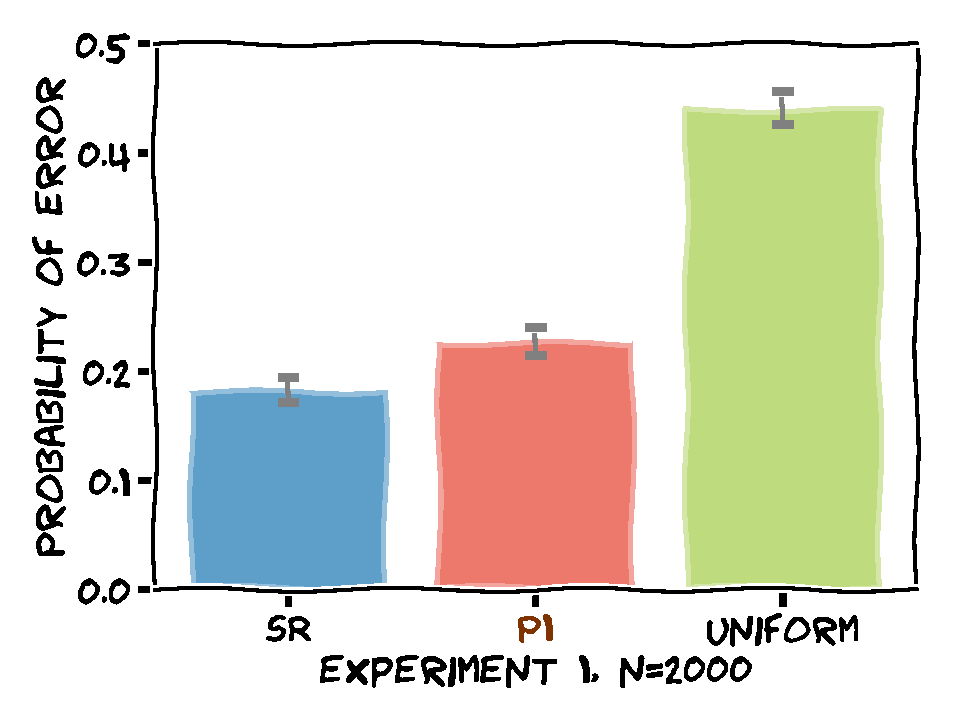
\includegraphics[width =.46\textwidth]{./image/exp1.pdf}$\qquad$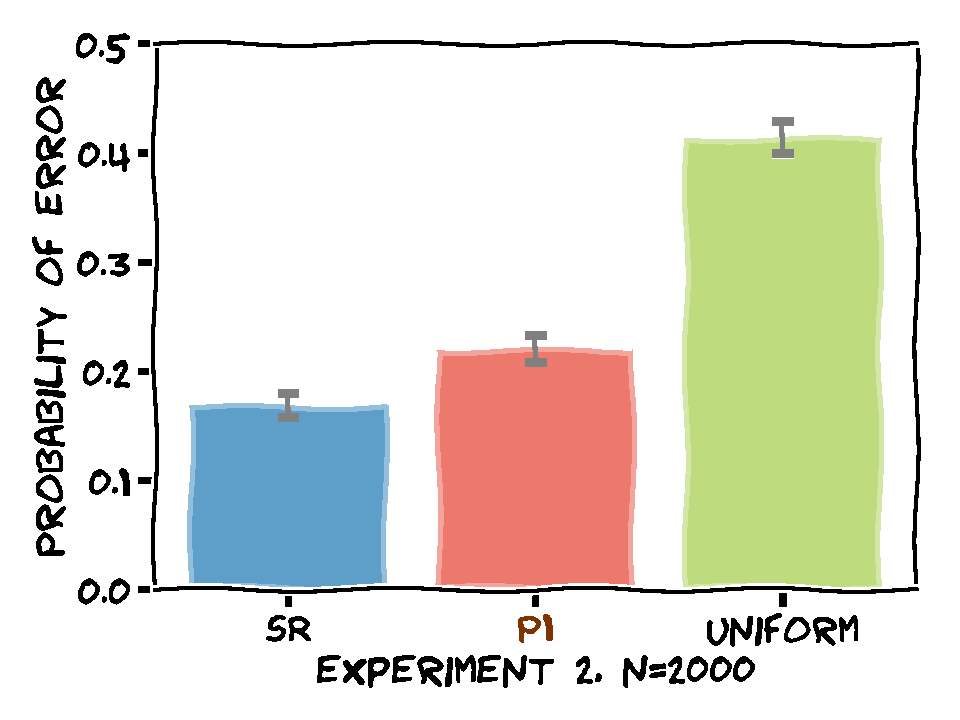
\includegraphics[width =.46\textwidth]{./image/exp2.pdf}
		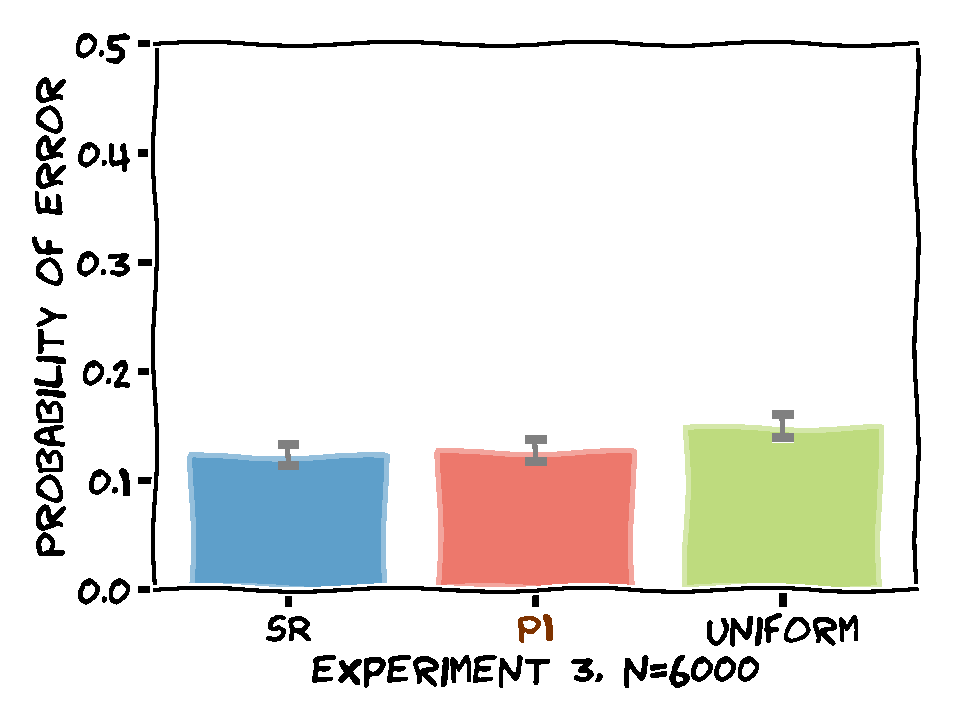
\includegraphics[width =.46\textwidth]{./image/exp3.pdf}$\qquad$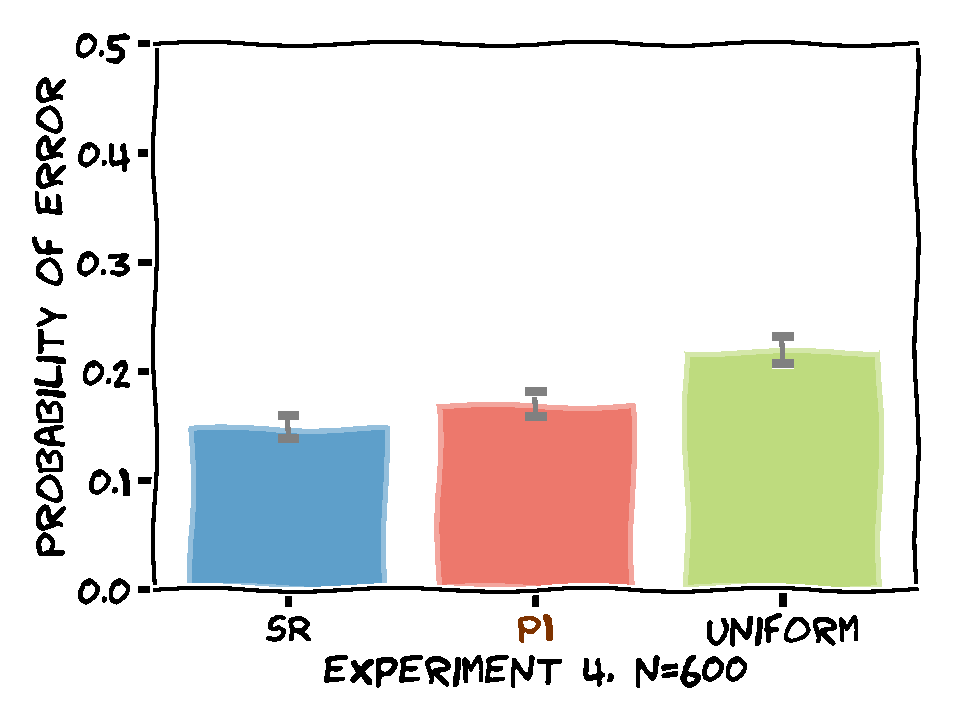
\includegraphics[width =.46\textwidth]{./image/exp4.pdf}
			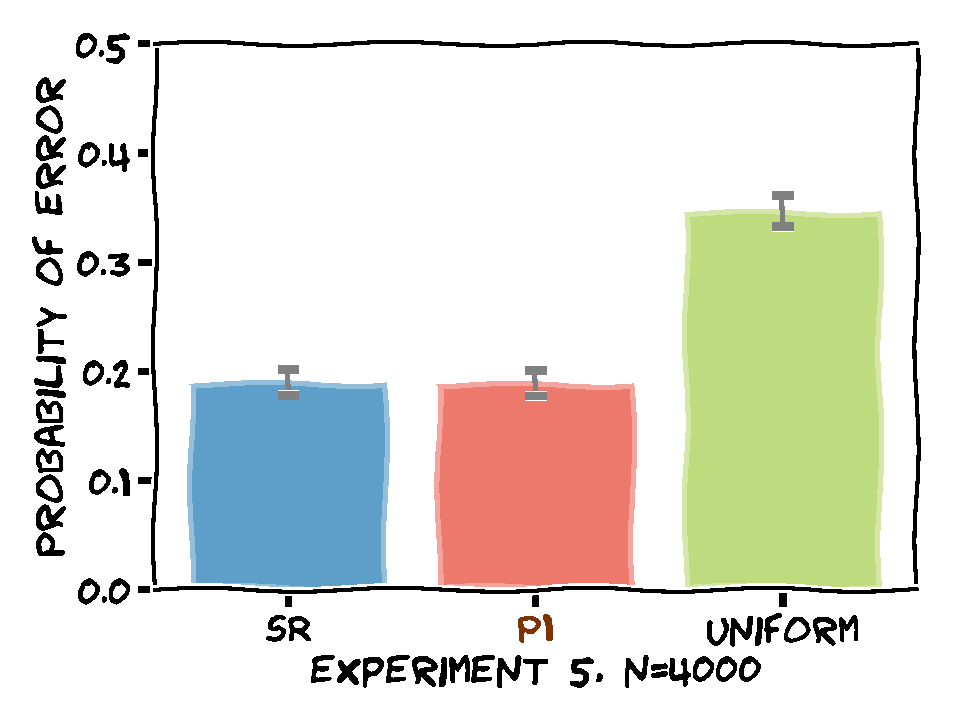
\includegraphics[width =.46\textwidth]{./image/exp5.pdf}$\qquad$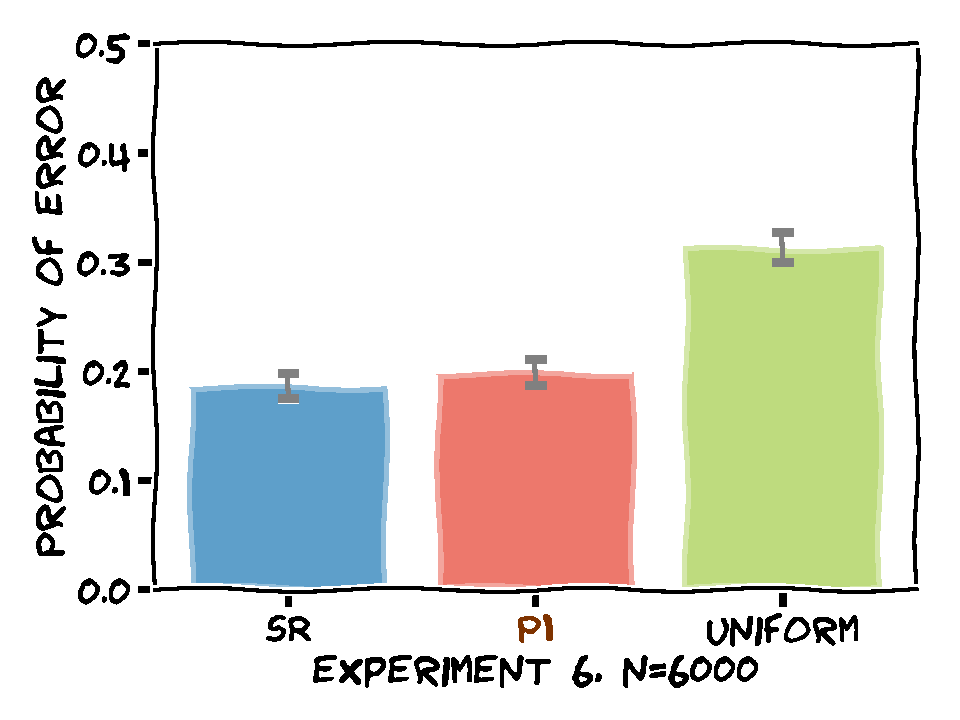
\includegraphics[width =.46\textwidth]{./image/exp6.pdf}
				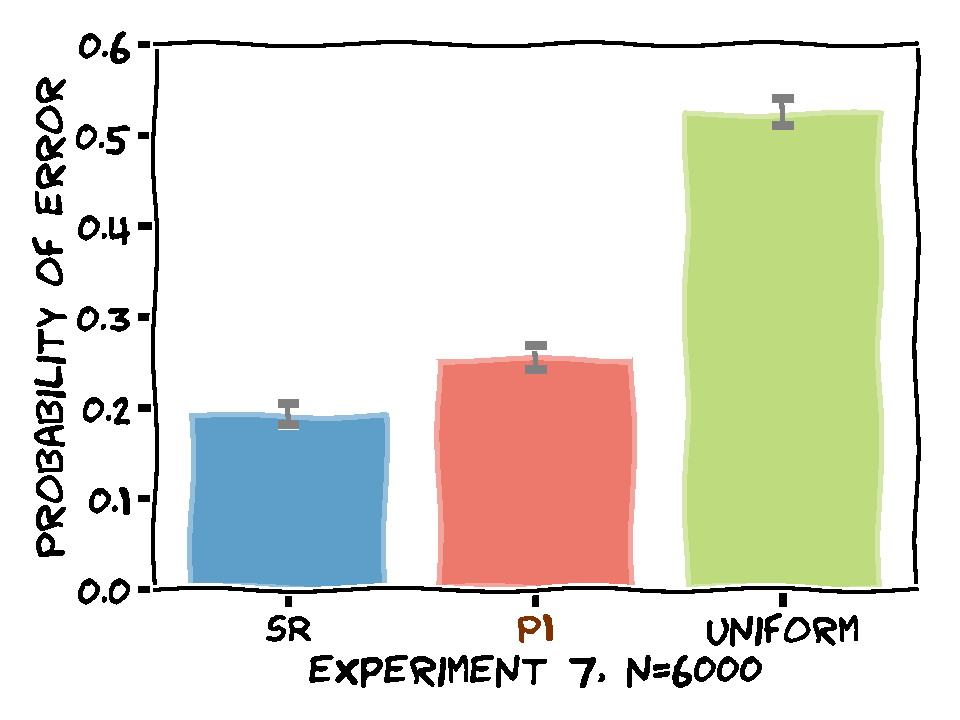
\includegraphics[width =.46\textwidth]{./image/exp7.pdf}$\qquad$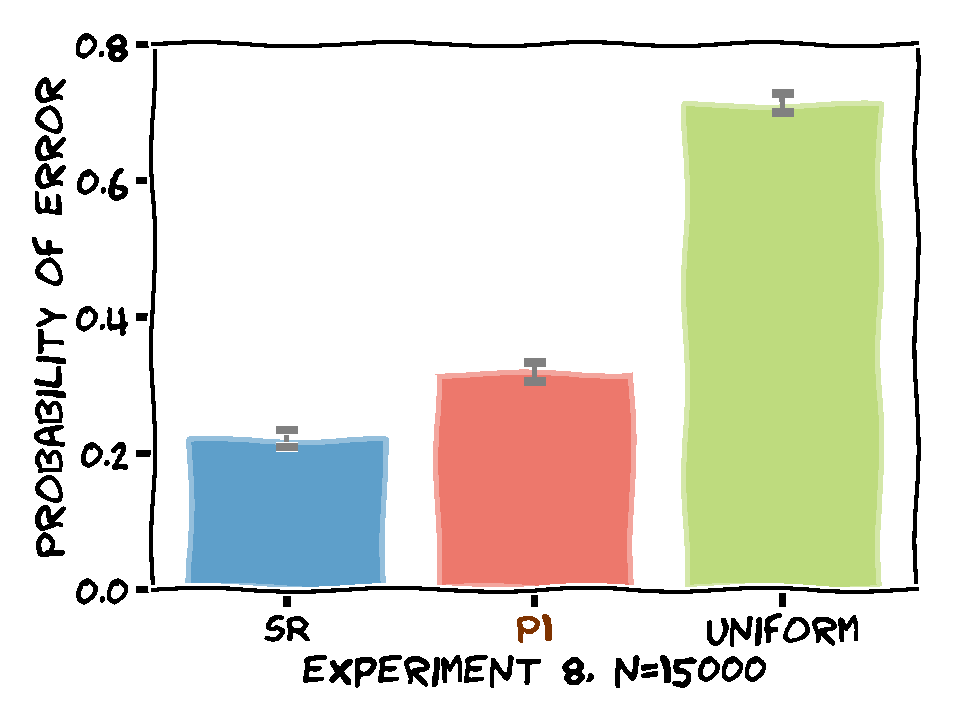
\includegraphics[width =.46\textwidth]{./image/exp8.pdf}
				\caption{Probabilities of error of \SR, \Pone, and the static uniform allocation.}\label{exp}
\end{figure}

%
\noindent In the remained of the appendix, for  a random variable $X$, we denote its variance  by $\var_X$.
Moreover, we also write that a bounded random variable
$X\in [\lowBrv_X,\upBrv_X]$  has a range $\range_X=\upBrv_X-\lowBrv_X.$ 
%\todom{this is kinda outta place now, depending on the spacing move before A
%otherwise start with the introductory " "}
%\todom{change to $\ell$}
% !TEX root = Main.tex 
\section{Upper bound on the probability of error of \RULE{} in the 
	general adversarial case} %(Theorem~\ref{th:UPARU}) }
\label{app:proofupadPRO}
%
\setcounter{scratchcounter}{\value{theorem}}\setcounter{theorem}{\the\numexpr\getrefnumber{th:UPARU}-1}
\tata*
\setcounter{theorem}{\the\numexpr\value{scratchcounter}}
\begin{proof}%[Theorem~\ref{th:UPARU}]
	%
	%To avoid technicalities and ease the reading, we henceforth assume that
	%    $\nArms$ is a power of $2$. %$K=\log(\TphaseNumber)$.
	We assume that the arms are sorted by their means 
	so that arm $1$ is the best.    
	Given the adversary gain vector $\gainVector$, the 
	random variables $\estGainVector_{k,t}$ are conditionally 
	independent from each other for all $k\in\setArms$ and 
	$t\in[\timeHorizon]$ as we have $\learnerDist_{k,t} 
	\triangleq 1/\nArms$, fixed for all 
	$k\in\setArms$ and $t\in[\timeHorizon]$.
	%we know that their variance is \todov{here the variance is just with respect to the learner should we include the adversary or condition somehow?}
	%
	%\todomi{do we need the stuff after or in the second like below?}
	We have
	\begin{align*}
	\ProErr_{\advPro(\gainVector)}(\timeHorizon)
	%    ~=~
	%        \ProErr_{\gainVector}(\timeHorizon)
	&\triangleq
	\Pro\left(  \recomArm_\timeHorizon \neq \bestArm_\gainVector\right)
	=    
	\Pro\left(\exists k\in\setArmsmo :
	\estCumulGainVector_{1,\timeHorizon} 
	\geq\estCumulGainVector_{k,\timeHorizon}
	\middle|\,\gainVector
	\right)\\
	&    \leq
	\Pro\left(\exists k\in\setArmsmo :\estCumulGainVector_{k,\timeHorizon} -\cumulGain_{k}\geq\frac{\timeHorizon\gap^\gainVector_{k}}{2} 
	\text{\ \ or\ \ }
	\estCumulGainVector_{1,\timeHorizon} -\cumulGain_{1}
	\leq\frac{\timeHorizon\gap^\gainVector_{1}}{2} 
	\middle|\,\gainVector
	\right)    \\
	&    \leq  
	\Pro\left(\estCumulGainVector_{1,\timeHorizon} -\cumulGain_{1}
	\leq\frac{\timeHorizon\gap^\gainVector_{1}}{2} \middle|\,\gainVector
	\right)    +
	\sum_{k=2}^{\nArms} 
	\Pro\left(\estCumulGainVector_{k,\timeHorizon} -\cumulGain_{k}
	\geq\frac{\timeHorizon\gap^\gainVector_{k}}{2} \middle|\, \gainVector
	\right)    \\
	&    \stackrel{\textbf{(a)}}{\leq} \sum_{k=1}^{\nArms} 
	\exp\left(-\frac{3(\gap^\gainVector_{k})^2\timeHorizon}
	{28\nArms}\right)\\
	&\leq \nArms  \exp\left(-\frac{3(\gap^\gainVector_{1})^2\timeHorizon}
	{28\nArms}\right)\!\CommaBin
	\end{align*}
	%
	where \textbf{(a)} is using Bernstein's inequality 
	applied to the sum of the random variables with mean zero 
	that are $\estGainVector_{k,t}-\gainVector_{k,t}$ for 
	which we have the following  bounds on  the variance and range.
	The variance  of $ \estGainVector_{k,t}$ is the 
	variance of a scaled Bernoulli random variable 
	with parameter $1/\nArms$ and range 
	%
	$[0, \nArms\gainVector_{k,t}]$,
	therefore we have 
	$|\estGainVector_{k,t}-\gainVector_{k,t} |
	\leq \nArms$, 
	and 
	$\var_{\estGainVector_{k,t}-\gainVector_{k,t}}
	=    \var_{\estGainVector_{k,t}}=
	1/\nArms(1-1/\nArms)\nArms^2\gainVector_{k,t}^2\leq \nArms$.
	We also use $\gap^\gainVector_k\leq 1$, for all 
	$k\in\setArms$ so that we have for all $k\in\setArmsmo$ 
	(and a symmetrical argument for $k=1$), 
	%
	\begin{align*}
	%
	\Pro\left(\estCumulGainVector_{k,\timeHorizon} - 
	\estCumulGainVector_{k,\timeHorizon} -\timeHorizon
	\gap^\frac{\gainVector_k}{2}\leq -\frac{\timeHorizon\gap^\gainVector_k}{2}\right) 
	&\leq
	\exp\left(-\frac{(\gap^\gainVector_k/2)^2\timeHorizon^2/2}
	{\sum_{t=1}^{\timeHorizon}\var_{\estGainVector_{k,t}-\gainVector_{k,t}}+\frac{1}{6} \nArms \gap^\gainVector_k\timeHorizon }\right)\\
	%&\qquad\qquad \qquad\qquad
	&\leq 
	\exp\left(-\frac{(\gap^\gainVector_k)^2\timeHorizon^2/8}
	{\timeHorizon\nArms+\frac{1}{6} \nArms \timeHorizon }\right)\\
	&\leq 
	\exp\left(-\frac{(\gap^\gainVector_k)^2\timeHorizon^2/8}
	{\timeHorizon\nArms+\frac{1}{6} \nArms \timeHorizon }\right)\\
	&=
	\exp\left(-\frac{3(\gap^\gainVector_k)^2\timeHorizon}
	{28\nArms}\right)\!\cdot
	\end{align*}\!\vskip -0.8cm\end{proof}%
%    \todomi{Michal: we could have $3K$, instead of $8K$, no?\\
%    Victor: I made the computation clearer and now found a 40! do you agree?\\
%    Michal: 32! You forgot additional $(/2)$ in right term of the denominator
%    }
%
%
%
%
%
% !TEX root = Main.tex 
\section{Change of measure}
\label{app:changeMeasureLem}
%
\begin{lemma}[\textcolor{titleTh}{Change of measure}]\label{l:changeMeas}
	% 
	Let $\earlyPhase$ be a phase, i.e., a subset of rounds of 
	the game, $\earlyPhase\subset [\timeHorizon]$. Let us 
	consider two  bandit problems. In these two problems, at all rounds $t\in[\timeHorizon]$, and for all arms $k\in\setArms$, the rewards $\gainVector_{k,t}$ are sampled in a stochastic learner-oblivious independent fashion from a distribution $\nu_{k,t}$.
	We consider problems that for all rounds of the game only differ in the rewards of one arm $\refarm$ 
	during phase~$\earlyPhase$. For all $t\in\earlyPhase$, 
	in the two problems, the distribution of  arm $\refarm$ is a Bernoulli 
	(independent  of all the other events in the bandit game for any round $t\in\earlyPhase$) with 
	means $\mean^2_{\refarm}(t)\triangleq\mean^2_{\refarm}\triangleq 1/2+\gap$ 
	and $\mean^1_{\refarm}(t)\triangleq\mean^1_{\refarm}\triangleq1/2-\gap'$ respectively for the two problems, 
	where $1/8>\gap'\geq \gap \geq 0$. 
		The expectation and probability with respect to the
	learner and the samples of this problem $p$ are denoted by
	$\Exp_{p}$ and $\Pro_{p}$.
	Then, if we have an event $W$
	depending only on $\gainVector$ generated by the problems and the actions of the learner $\pulledArm_{[\timeHorizon]}$
	 %which includes an upper 
	%bound $B$  %\todom{event includes an upper bound? rewrite. maybe: event }
	when the number of rounds  arm $\refarm$ is 
	pulled during phase $\earlyPhase$ is upper-bounded by $B$, we have  %\todom{it is not clear what is the event}
	% on the number of times the arm $\refarm$ is 
	%pulled during phase $\earlyPhase$, we have 
	%\todom{first $\Pro_{1}$ should be $\Pro_{2}$ }
	%
	\[
	\Pro_{2}\left(W \right)
	\geq
	\frac{\Pro_{1}\left(W  \right)}{8}
	\exp\left(-16\left(\gap'\right)^2B\right)\!.
	\]
	%
\end{lemma}
%
\begin{proof}
	This lemma is a slight extension of  Lemma 12 
	by~\cite{Auer16AA} %(arxiv version) \todom{we can't refer to the published one? it disappeared from there?}
	which in turn is 
	based on the result of~\cite{Mannor04SC}. In the case of \cite{Auer16AA}, $\gap' \triangleq \gap$.
	%Our proof reuses mostly their results and arguments.
	
	For $p\in\{1,2\}$,
	let $\Pro_{p}$ 	and $\Exp_{p}$ 
	denote the probability and expectation with respect to 
	the  bandit
	problem $p$ defined above. 
	%	
	Let $\sumlemma\triangleq\sum_{t\in\earlyPhase} \gainVector_{\refarm,t}\indicator{\pulledArm_t=\refarm}$
		be the sum of rewards received when 
	playing arm $\refarm$ in phase
	$\earlyPhase$. Conditioned on the number of pulls of 
	$\refarm$ during phase $\earlyPhase$ that we denote 
	by  $\pullearlyPhase$, $\sumlemma$	
	is a binomial random variable with parameters
	$\pullearlyPhase$	and $\mean^p_{\refarm}$ in problem $p$.
	Hence, by \cite{Kaas80MM},
	$$
	\Pro_{1}\left(  \sumlemma \leq   \lfloor\pullearlyPhase (1/2-\gap')\rfloor
	\right) \leq \frac12\cdot
	$$
	
	\noindent
	Let $w$ denote  a particular realization of rewards
	$\gainVector_{k,t}$, $k\in\setArms$, $t\in \earlyPhase$, 
	and learner choices
	$\left\{\pulledArm_t\right\}_{t\in \earlyPhase}$. For any realization
	$w$,
	%\todom{we should say in the theorem claim that other arms are also stochastic}
	the probabilities
	$\Pro_{1}(w)$ 
	and
	$\Pro_{2}(w)$
	are related by
	%	
	\[
	\Pro_{2}(w)
	=
	\Pro_{1}(w)\frac{(1/2+\gap)^{\sumlemma(w)} (1/2-\gap)^{\pullearlyPhase(w)-\sumlemma(w)}
	}{
		(1/2-\gap')^{\sumlemma(w)} (1/2+\gap')^{\pullearlyPhase(w)-\sumlemma(w)}}\cdot
	\]
	%
	Also, since $\frac{1/2+\gap}{1/2-\gap'}\geq 1$ and both 
	the numerator and denominator of the previous fraction are 
	positive, then the function $x\mapsto\frac{1/2+\gap+x}{1/2-\gap'+x}$ 
	is non-increasing for $x\geq0$. Therefore, we have  
	%
	\[
	\frac{1/2+\gap}{1/2-\gap'}
	\geq
	 \frac{1/2+\gap+(\gap'-\gap)/2}{1/2-\gap'+(\gap'-\gap)/2}
	 =
	  \frac{1/2+(\gap'+\gap)/2}{1/2-(\gap'+\gap)/2}\cdot
	\]
	%
	Similarly, since $\frac{1/2-\gap}{1/2+\gap'}\leq 1$ 
	and both the numerator and denominator of the previous 
	fraction are positive, then the function 
	$x\mapsto\frac{1/2-\gap-x}{1/2+\gap'-x}$ is non-increasing 
	for $1/2-\gap\geq x\geq0$. Therefore, choosing 
	$x=(\gap'-\gap)/2$, which verifies $x=(\gap'-\gap)/2\leq 1/2-\gap$ we have  that
	% 
	\[
	\frac{1/2-\gap}{1/2+\gap'}
	\geq
	 \frac{1/2-\gap-(\gap'-\gap)/2}{1/2+\gap'-(\gap'-\gap)/2}
	 =
	  \frac{1/2-(\gap'+\gap)/2}{1/2+(\gap'+\gap)/2}\cdot
	\]
%	
	Therefore, we have 
	%
	\begin{align*}
	\Pro_{2}(w)
	&\geq
	\Pro_{1}(w)
	\frac{(1+\gap+\gap')^{\sumlemma(w)} (1-\gap-\gap')^{\pullearlyPhase(w)-\sumlemma(w)}
	}{
		(1-\gap'-\gap)^{\sumlemma(w)} (1+\gap'+\gap)^{\pullearlyPhase(w)-\sumlemma(w)}}\\
	&=
	\Pro_{1}(w)
	\left(\frac{1-\gap-\gap'}{1+\gap+\gap'}\right)
	^{\pullearlyPhase(w)-2\sumlemma(w)}
	\geq
	\Pro_{1}(w)
	\left(\frac{1-2\gap'}{1+2\gap'}\right)^{\pullearlyPhase(w)
		-2\sumlemma(w)}\hspace{-4.5em}\cdot
	\end{align*}
	%
	If 	$ \sumlemma(w) \geq \lfloor\pullearlyPhase(w) (1/2-\gap')\rfloor$, then
	$\Pro_{2}(w)
	\geq
	\Pro_{1}(w)
	\left(\frac{1-2\gap'}{1+2\gap'}\right)^{2\gap'\pullearlyPhase(w)+2}\hspace{-4em}\cdot$
	
	%\todov{write the following better}
	\noindent
	Hence,
	\begin{align*}
	\Pro_{2}\left(W \right)
	&\geq
	\Pro_{2}\left(W  \cap \sumlemma \geq \lfloor\pullearlyPhase (1-\gap')\rfloor\right)\\
	&\geq
	\Pro_{1}\left(W  \cap \sumlemma \geq \lfloor\pullearlyPhase (1-\gap')\rfloor\right)
	\left(\frac{1-2\gap'}{1+2\gap'}\right)^{2\gap'B+2}\\
	&\geq
	\frac{\Pro_{1}\left(W  \right)}{2}
	\left(\frac{1-2\gap'}{1+2\gap'}\right)^{2\gap'B+2}\\
	&\geq
	\frac{\Pro_{1}\left(W  \right)}{2}
	\left(1-4\gap'\right)^{2\gap'B+2}\\
	&\stackrel{\textbf{(a)}}{\geq}
	\frac{\Pro_{1}\left(W  \right)}{8}
	\exp\left(-16(\gap')^2B\right)\!,
	\end{align*}
	where \textbf{(a)} is because for $0\leq x\leq 1/2$, $1-x\geq e^{-2x}$ and $\gap'\leq 1/8$.
%	
\end{proof}%
%
% !TEX root = Main.tex
\section{Lower bound in the general adversarial setting} %(Theorem~\ref{th:LOWadPRO}) }
\label{app:prooflowadPRO}
%
	\setcounter{scratchcounter}{\value{theorem}}\setcounter{theorem}{\the\numexpr\getrefnumber{th:LOWadPRO}-1}
\toto*
\setcounter{theorem}{\the\numexpr\value{scratchcounter}}
\begin{proof}%[Theorem~\ref{th:LOWadPRO}]
	Without loss of generality, we assume that $n$ is even.
	Let $\pullsNumber_{k}(t)$ be the number of times that arm 
	 $k$ has been pulled by the end of round $t$.
	%
	Let us consider any fixed learner and a base problem, denoted \basePro{}, with $\nu_1,\ldots, \nu_\nArms$, 
	Bernoulli distributions with means $\mean^{\basePro}_1,\ldots, \mean^{\basePro}_\nArms$ 
	such that $\mean^{\basePro}_1\triangleq 1/2$, and for all $k\in[2,\nArms], \mean^{\basePro}_k\triangleq1/2-\gap_k$ 
	(the gaps specified in the claim of the theorem).
		The expectation and probability with respect to the
	learner and the samples of this problem are denoted
	$\Exp_{\basePro}$ and $\Pro_{\basePro}$.% with $\gap_k\geq 0$ for .
	
	We consider  an early  period of the game $t=1, \dots, \timeHorizon/2$,\
	that we denote as $\earlyPhase\triangleq[1: \timeHorizon/2]$. %	
	The proof could work with any set of $\timeHorizon/2$ 
	rounds that are not necessarily the first of the game 
	but we stick to the early ones to ease the notation.
	Now we want to identify an arm that the learner will 
	not pull
	very much in the base problem \basePro{}
	during the period $\earlyPhase$.
	For our learner, during the period~$\earlyPhase$, in 
	any case at least one \emph{fixed} arm  among $\setArmsmo$ is pulled 
	in expectation % \todom{why in expectation? not always?} 
	less or equal to   
	$ \timeHorizon/\nArms $ as otherwise the total 
	number of pulls
	is in expectation strictly larger than $(\nArms-1)\times\timeHorizon/\nArms \geq \timeHorizon/2$. 
	We denote this arm as~$\refarm$. By this construction we have that
	%
	\begin{equation}\label{eq:notSoMuchPullsAD}
	\Exp_{\basePro}\left[\pullsNumber_{\refarm}\left(\frac{n}{2}\right) \right]
%		\pullsNumber_{\refarm}(n_i) 
	\leq  \frac{\timeHorizon}{\nArms}\cdot
	\end{equation}
	%
%	\todomi{what is $i$ in $n_i$?}
	Now we construct the two adversarial problems $\advPro_1$ and  $\advPro_2$.
	These adversarial problems sample  $\gainVector$ randomly.
	 During phase $\earlyPhase$, at rounds $t\in\earlyPhase$, 
	 for any arm $k$, $g_{k,t}$ is sampled from the Bernoulli 
	 distribution with means $\mu_{k}^{p}(t)$, $p\in\{1,2\}$ 
	 specifying the problem at hand.
	The expectation and probability with respect to the
	learner and the samples of this problem $p$ are denoted by
	$\Exp_{p}$ and~$\Pro_{p}$.
	
	
	For problem $\advPro_1$, the distributions of 
	the arms during phase $\earlyPhase$, $t\in\earlyPhase$, 
	are the same as in the \basePro{} 
	$\mu^{1}_{k}(t) \triangleq \mu^{\basePro}_{k} $ 
	for all $k\in \setArms$.
	After  phase $\earlyPhase$, for $t>  \timeHorizon/2$, 
	problem $\advPro_1$ assigns deterministically the following gains,
	 for all $k\neq \refarm$, for $t>  \timeHorizon/2$, $\gainVector_{k,t}=0$ 
	 and $\gainVector_{\refarm,t}=\gap_{\refarm}-\gap_1$.
	Therefore, the final expected cumulative gain of arm 
	 $\refarm$ is  \[\Exp_1\left[\cumulGain_{\refarm,n}\right]
	= \frac{\timeHorizon}{2}\mean^{\basePro}_{\refarm}+
	\frac{\timeHorizon}{2}\left(\gap_{\refarm}-\gap_1\right)=
	\frac{\timeHorizon}{2}\left(\mean^{\basePro}_1-\gap_1\right)\] and $\Exp_1\left[\cumulGain_{k,n}\right]= 
	\timeHorizon\mean^{\basePro}_k/2$ for all $k\neq\refarm$.
	The problem $\advPro_2$ only differs from the 
	previous one in its stochastic first part 
	(the deterministic second part is the same) and only for arm $\refarm$ where, 
	for $t\leq  \timeHorizon/2$, where $\mu_{\refarm}^{2}(t)\triangleq\mu_{\refarm}^{\basePro}+2\gap_1$.
	Therefore, the final expected cumulative gain of arm $\refarm$  
	is  \[\Exp_2\left[\cumulGain_{\refarm,n}\right]
	= \frac{\timeHorizon}{2}\left(\mean^{\basePro}_1+\gap_1\right).\] 
	
	
%	We denote the expected cumulative gain in problem $p$ of each arm $k\in\setArms$ as $\expectCumul_{k}=\sum_{t=1}^{\timeHorizon} \mean^{\advPro}_{k}(t)$. \todo{do something with notation here, maybe define outside!}
	
	\noindent
	%\todomi{$p$ is free variable here! for all $p$ or for one fixed or what?}
	Let us consider the events
	%
	\begin{align*}
	\eventc_1 &\triangleq \left\{ \forall k\in\setArmsmo,~  \cumulGain_{k}-
	\Exp_1\left[\cumulGain_{k}\right] \leq  \frac{\timeHorizon \gap_1}{8} \right\} 
	\cup \left\{  \Exp_1\left[\cumulGain_{1}\right]-\cumulGain_{1} 
	\leq  \frac{\timeHorizon \gap_1}{8} \right\} \text{\ and}\\
%	\]
	%
%	
	% 
%		\[
	\eventc_2 &\triangleq \left\{ \forall k\in\setArms, k\neq \refarm,~   
	\cumulGain_{k}-\Exp_2\left[\cumulGain_{k}\right] \leq  \frac{\timeHorizon \gap_1 }{8}
	\right\} \cup \left\{  \Exp_2\left[
	\cumulGain_{\refarm}\right]-\cumulGain_{\refarm} \leq  \frac{\timeHorizon \gap_1 }{8}\right\}\!\cdot
	\end{align*}
	% 
	Using a standard Hoeffding argument with a 
	union bound we have that 
	%\todomi{here we implicitly assume that both the games are run in parallel}
	%
	\[
	\Pro_1\left(\eventc_1\right) \geq 1-\nArms\exp\left(
	-2\left(\frac{\gap_1}{8}\right)^2\frac{\timeHorizon}{2}\right)
	\] %\todom{we don't need the last $1/2$, right? the r.v. are Bernoullis}
	and the same result holds for $\Pro_2\left(\eventc_2\right)$.
	%
	Also note that  in the  problem $p$, for 
	any $\gainVector$ that is compatible with 
	$\eventc_p$, the gaps associated to $\gainVector$ verify
	$\gap_k/2\leq\gap^{\gainVector}_k\leq 3 \gap_k$ for all $k\neq \refarm$
	and $\gap_1/2\leq\gap^{\gainVector}_{\refarm}\leq2\gap_1$
which gives $4\complexityUnif\geq\complexityUnif(\gainVector)\geq
 \complexityUnif/9$. Also on $\gainVector\in\eventc_1$, 
 we have $\bestArm_\gainVector=1$ and  on $\gainVector\in\eventc_2$, we have $\bestArm_\gainVector=\refarm$.
	
	
	Now we prove the following relation 
	between the probability of error 
	in the  problem $\advPro_2$, $\ProErr_{2}(\timeHorizon)$, and the
	probability of successful identification in the  problem $\advPro_1$,
	$1-\ProErr_{1}(\timeHorizon)$,
	where in this case, for problem $p$, $\ProErr_{p}(\timeHorizon)$ 
	%\todomi{here the "adversarial sampling" notation makes a cameo}
	is defined here as $\ProErr_{p}(\timeHorizon) \triangleq
	 \Pro_{\gainVector\sim \advPro_p}\left(\recomArm_n \neq \bestArm_{\gainVector}\right)$,
	% 
		\begin{equation}\label{eq:mainlowGenAd}
	\ProErr_{2}(\timeHorizon)
	+\nArms\exp\left(-\frac{\gap^2_1\timeHorizon}{64}\right)
	\geq
	\frac{1}{8}\left(\frac{1}{4}-\ProErr_{1}(\timeHorizon) \right)
	\exp\left(-\frac{32\gap^2_{1}\timeHorizon}{\nArms}\right)\!\cdot
	\end{equation}
	%
	We have that
	%
	\begin{align*}
	\ProErr_{2}(\timeHorizon)
	+\nArms\exp\left(-\frac{\gap^2_1\timeHorizon}{64}\right)
	&\stackrel{\textbf{(a)}}{\geq}
	\Pro_{2}\left(\recomArm_\timeHorizon\neq \refarm\right)\\
	&\stackrel{\textbf{(b)}}{\geq}
	\Pro_{2}\left(\recomArm_\timeHorizon=1\right)\\
	&\stackrel{\textcolor{white}{\textbf{(b)}}}{\geq}
	\Pro_{2}\left(\recomArm_\timeHorizon=1 \cap \pullsNumber_{\refarm} \left(\frac{\timeHorizon}{2}\right) 
	\leq \frac{2\timeHorizon}{\nArms} \right)\\
	&\stackrel{\textbf{(c)}}{\geq}
	\Pro_{1}\left(\recomArm_\timeHorizon=1 \cap \pullsNumber_{\refarm} \left(\frac{\timeHorizon}{2}\right) 
	\leq \frac{2\timeHorizon}{\nArms} \right)\frac{1}{8}\exp\left(-\frac{16\gap^2_{1}2\timeHorizon}{\nArms}\right)\\
	&\stackrel{\textbf{(d)}}{\geq}
	\left(\Pro_{1}\left(\recomArm_\timeHorizon=1 \right)-\frac{1}{2}\right)\frac{1}{8}
	\exp\left(-\frac{32\gap^2_{1}\timeHorizon}{\nArms}\right)\\
	&\stackrel{\textbf{(a)}}{\geq}
	\frac{1}{8}\left(\frac{1}{4}-\ProErr_{1}(\timeHorizon) \right)
	\exp\left(-\frac{32\gap^2_{1}\timeHorizon}{\nArms}\right)\!\CommaBin
	\end{align*}
	%
	where 
	\textbf{(a)} %\todo{maybe no need for this depending on the definition of the best arm} 
	is because first, as computed above, 
	for problem $p$,
	\[\Pro_{ p}\left(\bestArm_{\gainVector}=1\right)\geq \Pro(\eventc_p) 
	\geq 1-\nArms\exp\left(-\frac{\gap^2_1\timeHorizon}{64}\right)\!\CommaBin\] 
	since; if we denote $1^\star=1$ (the arm with the highest mean in $p=1$) %\todom{correct?}  
	and $2^\star=\refarm$ (the arm with the highest mean in  $p=2$)
	and in general $p^\star$, we have that
	%
	\begin{align*}	
	\ProErr_{p}(\timeHorizon)
	&=
	1- \Pro_{p}\left(\recomArm_\timeHorizon=\bestArm_{\gainVector}\right)
	=
	1- \Pro_{p}\left(\recomArm_\timeHorizon=\bestArm_{\gainVector} 
	\cap \bestArm_{\gainVector}=p^\star\right)
	- \Pro_{p}\left(\recomArm_\timeHorizon=\bestArm_{\gainVector}
	\cap\bestArm_{\gainVector}\neq p^\star\right)\\
&	\geq
	1-
	\Pro_{p}\left(\recomArm_\timeHorizon=p^\star\right)
	- \Pro_{p}\left(\bestArm_{\gainVector}\neq p^\star\right)
		\geq
	1-
	\Pro_{p}\left(\recomArm_\timeHorizon=p^\star\right)
	- \nArms\exp\left(-\frac{\gap^2_1\timeHorizon}{64}\right)\!\cdot
	\end{align*}
	Moreover, 
	$\nArms\exp\left(-\gap^2_1\timeHorizon/64\right) \leq 1/4$ 
	by an assumption of the theorem.
%	
	Next, \textbf{(b)}  is because we have $1\neq\refarm$ 
	by construction and
	\textbf{(c)} uses the change-of-measure 
	argument from Lemma~\ref{l:changeMeas}. % \todo{do we need somethingabout Jn being a deterministic function so that we can use the lemma on events?} \todov{explained in a separate lemma becuase we might be able to have something that we could reuse for the lower bound of the general case above}
	Finally, \textbf{(d)} is because 
	%
	\begin{align*}
	\Pro_{1}\left(\recomArm_\timeHorizon=1 \right)
	&=
	\Pro_{1}\left(\recomArm_\timeHorizon=1 \cap \pullsNumber_{\refarm} \left(\frac{\timeHorizon}{2}\right) 
	\leq \frac{2\timeHorizon}{\nArms} \right)
	+
	\Pro_{1}\left(\recomArm_\timeHorizon=1 \cap 
	\pullsNumber_{\refarm} \left(\frac{\timeHorizon}{2}\right) 
	> \frac{2\timeHorizon}{\nArms} \right)\\
	&\leq
	\Pro_{1}\left(\recomArm_\timeHorizon=1\cap \pullsNumber_{\refarm} \left(\frac{\timeHorizon}{2}\right) 
	\leq \frac{2\timeHorizon}{\nArms} \right)
	+
	\Pro_{1}\left( \pullsNumber_{\refarm} \left(\frac{\timeHorizon}{2}\right) 
	> \frac{2\timeHorizon}{\nArms} \right)\\
	&\leq
	\Pro_{1}\left(\recomArm_\timeHorizon=1 \cap \pullsNumber_{\refarm} \left(\frac{\timeHorizon}{2}\right) 
	\leq \frac{2\timeHorizon}{\nArms} \right)
	+
	\frac12\CommaBin
	\end{align*}
	%
	where the last inequality combines Equation~\ref{eq:notSoMuchPullsAD} 
	and Markov's inequality.
	
%\smallskip	\noindent
\paragraph{Two cases}
After proving Equation~\ref{eq:mainlowGenAd}, we	finally 
	 distinguish two cases. \\
	%\bigskip 
	\noindent\textbf{Case 1) $\ProErr_{2}(\timeHorizon)>
		\exp\left(-32\gap^2_{1}\timeHorizon/\nArms\right)\!/64$:}
	%
%	We have
%	%
%	\begin{align*}
%	\frac{1}{64}\exp\left(-32\gap^2_{1}\timeHorizon/\nArms\right)
%	&~\stackrel{(a)}{\geq}~
%	4\nArms\exp\left(-\gap^2_{1}\timeHorizon/128\right)\exp\left(-32\gap^2_{1}\timeHorizon/\nArms\right)\\
%		&~\stackrel{(b)}{\geq}~
%4\nArms\exp\left(-\gap^2_{1}\timeHorizon/128\right)\exp\left(-\gap^2_{1}\timeHorizon/128\right)
%	\end{align*}
%	%
%	where \textbf{(a)} is because by assumption we have  $8\nArms\exp\left( -\timeHorizon\gap^2_1 /128\right)\leq 1/16$ and
%	\textbf{(b)} is because by assumption we have  $\nArms>32\times128$.
%	
%	Therefore 
%$\ProErr_{2}(\timeHorizon)>
%\frac{1}{64}\exp(-32\gap^2_{1}\timeHorizon/\nArms)$
%	then 	
%	$\ProErr_{2}(\timeHorizon)>
%	4\nArms\exp\left(-\frac{\gap^2_1\timeHorizon}{64}\right)$.
		We claim  there exists $\gainVector\in\eventc_2$,  
	as discussed above,  that its best arm is  $\refarm$ and it 
	possesses a complexity verifying $4\complexityUnif\geq\complexityUnif(\gainVector)\geq \complexityUnif/9$,  
	such that the lower bound holds. We prove the statement by contradiction.
	Indeed if no $\gainVector\in\eventc_2$ is such that 
$
\ProErr_{\gainVector}(n)
	\geq
	 \exp( -\timeHorizon32\gap^2_1 /\nArms)/128,
$	then we have 
%\todomi{equality in the second line}
%\todomi{$p$ should be 2 below}
	\begin{align*}
	\ProErr_{2}(\timeHorizon)
&=
\Pro_{\gainVector\sim \advPro_2}\left(\recomArm_n \neq \bestArm_{\gainVector}\right)\\
&\leq
\Pro\left(\recomArm_n \neq \bestArm_{\gainVector}\cap\gainVector\in\eventc_2\right)
+
\Pro\left(\recomArm_n \neq \bestArm_{\gainVector}\cap\gainVector\notin\eventc_2\right)\\
&\leq
\Pro\left(\recomArm_n \neq \bestArm_{\gainVector}\cap\gainVector\in\eventc_2\right)
+
\Pro\left(\gainVector\notin\eventc_2\right)\\
&\leq
 \frac{1}{128}\exp\left( -\frac{\timeHorizon32\gap^2_1 }{\nArms}\right)
+
\nArms\exp\left(-\frac{\gap^2_1\timeHorizon}{64}\right)\\
 &=
 \frac{1}{128}\exp\left( -\frac{\timeHorizon32\gap^2_1 }{\nArms}\right)
 +
\nArms\exp\left(-\frac{\gap^2_1\timeHorizon}{128}\right)\exp\left(-\frac{\gap^2_1\timeHorizon}{128}\right)\\
 &\stackrel{\textbf{(a)}}{\leq}
   \frac{1}{128}\exp\left( -\frac{\timeHorizon32\gap^2_1 }{\nArms}\right)
 +
 \frac{1}{128}\exp\left( -\frac{\timeHorizon\gap^2_1}{128}\right)\\
 &\stackrel{\textbf{(b)}}{\leq}
 \frac{1}{128}\exp\left( -\frac{\timeHorizon32\gap^2_1 }{\nArms}\right)
 +
 \frac{1}{128}\exp\left( -\frac{\timeHorizon32\gap^2_1 }{\nArms}\right)\!\CommaBin
\end{align*}
where \textbf{\textbf{(a)}} is because
$\nArms\exp\left( -\timeHorizon\gap^2_1 /128\right)\leq 1/128$ 
 and 
 \textbf{(b)}
because $\nArms>32\times128$
 by assumptions.
	This is a contradiction with the original assumption of that case.
	

	%%%%%%%%%%%%%%%%%%%%%%%%%%%%%%%%%%%%%
		\smallskip	
	\noindent\textbf{Case 2) $\ProErr_{2}(\timeHorizon)\leq
	\exp(-32\gap^2_{1}\timeHorizon/\nArms)/64$:}
We first want to prove that this assumption gives
	%
	\begin{equation}\label{eq:lowbobcase2}
\ProErr_{1}(\timeHorizon)\geq \frac{1}{16}\CommaBin
	\end{equation}
	that we prove by first using Equation~\ref{eq:mainlowGenAd} which gives
	\[
		\frac{1}{64}\exp\left(-\frac{32\gap^2_{1}\timeHorizon}{\nArms}\right)
		+
		\nArms\exp\left(-\frac{\gap^2_1\timeHorizon}{64}\right)
		\geq
		\frac{1}{8}\left(\frac{1}{4}-\ProErr_{1}(\timeHorizon) 
		\right)\exp\left(-\frac{32\gap^2_{1}\timeHorizon}{\nArms}\right)\!\CommaBin
%\ProErr_{2}(\timeHorizon)\geq 1/8 - 64\nArms\exp\left(-\frac{\gap^2_1\timeHorizon}{8}\right) / \exp(-32\gap^2_{1}\timeHorizon/\nArms) 
%=1/8-64\nArms\exp\left( \timeHorizon\gap^2_1 (32/\nArms-1/8)  \right)
%\geq 1/8-64\nArms\exp\left( -\timeHorizon\gap^2_1 /16)  \right)
%\geq 1/16
	\]
and hence
	\[
\frac{1}{8}
+
8\nArms\frac{\exp\left(-\frac{\gap^2_1\timeHorizon}{64}\right)}
{\exp\left(-\frac{32\gap^2_{1}\timeHorizon}{\nArms}\right)}
\geq
\frac{1}{4}-\ProErr_{1}(\timeHorizon). 
\]
Therefore, we have 	
	\begin{align*}
\ProErr_{1}(\timeHorizon) 
&\geq
\frac{1}{8}
-
8\nArms\exp\left(\frac{32\gap^2_{1}\timeHorizon}{\nArms}-\frac{\gap^2_1\timeHorizon}{64}\right)\\
&\stackrel{\textbf{(a)}}{\geq}
\frac{1}{8}
-
8\nArms\exp\left(-\frac{\gap^2_1\timeHorizon}{128}\right)\\
&\stackrel{\textbf{(b)}}{\geq}
\frac{1}{16}\CommaBin
\end{align*}
%
where \textbf{(a)} is 
	because $\nArms>32\times128$ and
	\textbf{{(b)}} is because $\nArms\exp\left( -\timeHorizon\gap^2_1 /128\right)\leq 1/128$ by assumptions.	
	We now claim that there exists at least one~$\gainVector\in\eventc_1$   
	with best arm $1$  such that 
	$\ProErr_{\gainVector}(\timeHorizon)\geq 1/32$. 
	The proof is by contradiction. Let us assume that for all $\gainVector\in\eventc_1$, $\ProErr_{\gainVector}(\timeHorizon)< 1/32$. 
	%
	Then, we have 
	\begin{align*}
	%
\ProErr_{1}(\timeHorizon)
	&=
	\Pro_{\gainVector\sim\advPro_1}\left(\recomArm_n \neq 
	\bestArm_{\gainVector}\right)\\
	&=
	\Pro_{\gainVector\sim\advPro_1}\left(\recomArm_n \neq 
	\bestArm_{\gainVector}|\,\gainVector\in\eventc_1\right)
	P\left(\eventc_1\right)
	+
	\Pro_{\gainVector\sim\advPro_1}\left(\recomArm_n \neq 
	\bestArm_{\gainVector}|\,\gainVector\notin\eventc_1\right)
	P\left(\neg\eventc_1\right)\\
	&\leq
\frac{1}{32}
	\times 1
	+
	1\times
	\nArms\exp\left(-\frac{\gap^2_1\timeHorizon}{64}\right)\\
	&\leq
	\frac{1}{32}
	\times 1
	+
	1\times
	\frac{1}{128}\\
	&<
	\frac{1}{16}\CommaBin
	%
\end{align*} which contradicts Equation~\ref{eq:lowbobcase2}.
%
\end{proof}%
%
% !TEX root = Main.tex
%

\section{Lower bound in the best of both worlds} %setting (Theorem~\ref{th:lowBOB}) }
\label{app:prooflowBOB}
%
\setcounter{scratchcounter}{\value{theorem}}\setcounter{theorem}{\the\numexpr\getrefnumber{th:lowBOB}-1}
\thi*
\setcounter{theorem}{\the\numexpr\value{scratchcounter}}
\begin{proof}%[Theorem~\ref{th:lowBOB}]
	%    
	Let $\pullsNumber_{k}(t)$ be the number of times that arm 
	$k$ has been pulled by the end of round $t$.
	Let us consider any fixed learner.
	Let us consider a base problem, denoted \basePro{}, with $\nu_1,\ldots, \nu_\nArms$, 
	Bernoulli distributions with mean $\mean^{\basePro}_1,
	\ldots, \mean^{\basePro}_\nArms$ 
	such that $\mean^{\basePro}_1 \triangleq 1/2$, and for all $k\in[2,\nArms], 
	\mean^{\basePro}_k \triangleq  1/2-\gap_k$ 
	(the gaps specified in the claim of the theorem).
	The expectation and probability with respect to the
	learner and the samples of this problem are 
	$\Exp_{\basePro}$ and $\Pro_{\basePro}$.% with $\gap_k\geq 0$ for .
	
	Here, $i\in\setArmsmo$ denotes the rank of a suboptimal arm in the
	base problem. Next, we consider  a constant $\dividefac_i\leq 1$.
	We also consider  an early  period of the game $t=1,\ldots,
	\timeHorizon_i\triangleq\lceil \timeHorizon\dividefac_i\rceil$,\
	that we denote~$\earlyPhase_i$. %
	%    \todov{define with equal triangle}
	The proof could work with any set of $\timeHorizon_i$ rounds 
	that are not necessarily the first of the game but we stick 
	to the early ones to ease the notation.
	Now we want to identify an arm with a small gap that the 
	learner will not pull
	very much in the base problem \basePro{}
	during the period~$\earlyPhase_i$.
	From our learner, during the period $\earlyPhase_i$, 
	in any case at most 
	$i-2$ arms among $\setArmsmo$ %, noted $S$,  
	will, in expectation, be pulled strictly more than 
	$2\timeHorizon_i/i $ as otherwise the total number of pulls
	is strictly larger than $(i-1)\times2\timeHorizon_i/i\geq\timeHorizon_i$.
	Therefore, we have at least $\nArms-1-(i-2)=\nArms-i+1$ arms 
	included in the set $\setArmsmo$, 
	and that form a set
	noted $S$,  that are pulled in expectation less than $2\timeHorizon_i/i $.
	Among these arms, let us consider  arm $\refarm \triangleq \argmax_{k\in S}
	\mean_k$ with highest mean. By construction we have
	%
	\begin{equation}\label{eq:notSoMuchPulls}
	\Exp_{\basePro}\left[\pullsNumber_{\refarm}(n_i) \right]\leq \frac{2n_i}{i}\cdot
	\end{equation}
	%        
	Note that by construction, we have also that  $\gap_{\refarm}\leq\gap_i$, because
	otherwise it would mean that $\mean_{\refarm}<\mean_i$ 
	and so there would exist at most $\nArms-i-1$ arms with lower means than $\refarm$.
	This contradicts the fact that $\refarm$ has the highest 
	mean among $\nArms-i+1$ arms.
	
	
	Now we construct an i.i.d.\,stochastic problem, denoted \stoPro{}, where
	the distribution of the arms are the same as in the \basePro{} 
	problem  except for arm $\refarm$, $\mu^{\stoPro}_{k}\triangleq \mu^{\basePro}_{k} $ 
	for all $k\neq \refarm$.
	%    We distinguish two cases: if the  $\refarm=1$ then
	We set in  \stoPro{},         
	$\mu^{\stoPro}_{\refarm} \triangleq 1/2 + \gap_1/2$.
	This means that 
	the best arm in the \stoPro{} is the arm $\refarm$, $\bestArmSto\triangleq\refarm$.
	Also note that the gaps in the \stoPro{} problem verify
	$\gap_k\leq \gap^{\stoPro}_k=\gap_k+\gap_1/2\leq 2\gap_k$ for 
	all $k\in[2,\refarm-1]\cup[\refarm+1:\nArms]$. Also, $\gap_1= 
	\gap^{\stoPro}_1/2$ and $ \gap^{\stoPro}_{\refarm}=\gap_{1}/2$.
	Therefore,  \[\frac{\complexityBoth^{\basePro}}{2}
	\leq\complexityBoth^{\stoPro}\leq 8\complexityBoth^{\basePro}.\]
	The expectation and probability with respect to the
	learner and the samples of this problem are denoted
	$\Exp_{\stoPro}$ and $\Pro_{\stoPro}$.
	
	
	
	The second bandit problem is the adversarial one, denoted \advPro{}.
	This adversarial problem samples  $\gainVector$ randomly.
	At round $t\in[\timeHorizon]$, for arm $k$, $g_{k,t}$ is sampled 
	from the Bernoulli distribution with mean $\mu_{k}^{\advPro}(t)$.
	For all $t$ and $k\neq\refarm$, \advPro{} follows the \basePro{} 
	problem:  $\mu_{k}^{\advPro}(t)\triangleq\mu_{k}^{\basePro}$.
	For arm $\refarm$,
	until the end of phase $\earlyPhase_i$, for all $t$ with $1\leq 
	t\leq n_i$, $\mu^{\advPro}_{\refarm}(t)\triangleq\mu_{\refarm}^{\basePro}$ 
	and then a switch happens, for $n_i< t\leq n$, arm $\refarm$ 
	possesses  the same distributions as in the \stoPro{} problem,  
	$\mu^{\advPro}_{\refarm}(t)\triangleq \mu_{\refarm}^{\stoPro}$.
	The expectation and probability with respect to the
	learner and the samples of this problem are denoted
	$\Exp_{\advPro}$ and $\Pro_{\advPro}$.
	
	
	Let us now study the identity of the best arm in \advPro{}.
	We want to show that, with high probability, 
	the best arm in the \advPro{} is  arm $1$ if we have 
	$\dividefac_i\geq \gap_1/ \gap_i.$
	We denote the expected cumulative gain in \advPro{} of each 
	arm $k\in\setArms$ as $\expectCumul_{k}\triangleq\sum_{t=1}^{\timeHorizon} \mean^{\advPro}_{k}(t)$.
	%\todov{we need to lower bound the lowest mean by a constant to fix when things and constant gets clear}
	%\todov{check what is happening with the flooring of $\timeHorizon_i$,$\lfloor\rfloor\timeHorizon_i\rfloor$ }    
	For arm $\refarm$, we have 
	\begin{align*}    
	\expectCumul_{\refarm}&=
	\sum_{t=1}^{\timeHorizon_i} \mean^{\advPro}_{\refarm}(t)
	+
	\sum_{t=\timeHorizon_i+1}^{\timeHorizon} \mean^{\advPro}_{\refarm}(t)\\
	&=
	\timeHorizon_i \mean^{\basePro}_{\refarm}
	+
	(\timeHorizon-\timeHorizon_i) \mean^{\stoPro}_{\refarm}  \\
	&=
	\timeHorizon_i \left(\frac12 - \gap_i\right)
	+
	(\timeHorizon-\timeHorizon_i) \left(\frac12 + \frac{\gap_1}{2}\right)\\
	&\leq
	\frac{\timeHorizon}{2}-  \timeHorizon_i \gap_i
	+
	\frac{\timeHorizon \gap_1}{2}\ \\    
	&\leq    
	\frac{\timeHorizon}{2} - \dividefac_i\timeHorizon \gap_i
	+
	\frac{\timeHorizon \gap_1}{2}\\\
	&\leq    
	\frac{\timeHorizon}{2} - \timeHorizon \gap_1
	+
	\frac{\timeHorizon \gap_1}{2}\\\        
	&=    
	\frac{\timeHorizon}{2} - \frac{\timeHorizon \gap_1}{2}\cdot
	\end{align*}    
	%\todov{write this with better notation once they are fixed}
	For all $k\in\setArms$, $k\neq\refarm$ and $k\neq1$, we have $\expectCumul_{k}=     
	\timeHorizon/2 - \timeHorizon \gap_k$. Furthermore, $\expectCumul_{1}=     
	\timeHorizon/2$. 
	%    
	Let us consider the event
	$\eventc =\left\{ \forall k\in\setArms,  |\cumulGain_k-\expectCumul_{k}| \leq  \timeHorizon \gap_1/8 \right\}
	$.
	Using a standard Hoeffding argument with a union bound we have 
	that $\Pro(\eventc) \geq 1-\nArms\exp\left(-\gap^2_1\timeHorizon/32\right)$.
	Then, in the \advPro{} problem, for any $\gainVector$ that is 
	compatible with $\eventc$, the gaps associated with $\gainVector$ 
	verify
	$\gap_k/2\leq\gap^{\gainVector}_k\leq2\gap_k$ for all $k\neq 
	\refarm$ and $\gap_1/4\leq\gap^{\gainVector}_{\refarm}\leq\gap_1$.    
	Note that therefore the only difference between the two problems 
	\stoPro{} and \advPro{} is for  arm $\refarm$ during phase $\earlyPhase_i$.
	
	
	If we have $\dividefac_i\geq \gap_1 / \gap_i$,  then with high probability, the respective best arms 
	in problem \stoPro{} and problem \advPro{}
	are % \todom{rephrase} 
	different, i.e., $\bestArmAd\neq\bestArmSto$. That is what we assume for
	the rest of the proof. Indeed, we want to use the fact that 
	the two models are hard to differentiate from the learner point 
	of view with a certain probability and that then the learner has 
	to either choose to recommend $\bestArmAd$ or $\bestArmSto$, which are different, and therefore possibly suffer a mistake.
	
	
	%    \todo{talk about is $J_n$?}
	
	Then we prove the following relation between the probability of error 
	in the stochastic problem $\ProErr_{\stoPro}(\timeHorizon)$ to the
	probability of successful identification in the adversarial problem
	$1-\ProErr_{\advPro}(\timeHorizon)$:
	where $\ProErr_{\advPro}(\timeHorizon)$ is defined here as 
	$\ProErr_{\advPro}(\timeHorizon) \triangleq \Pro_{\gainVector\sim\advPro}\left(\recomArm_n \neq \bestArm_{\gainVector}\right)$,
	%
	\begin{equation}\label{eq:mainlowBOB}
	\ProErr_{\stoPro}(\timeHorizon)
	\geq
	\frac{1}{8}\left(\frac{1}{4}-\ProErr_{\advPro}(\timeHorizon) \right)\exp\left(-\frac{64\gap^2_{i}\timeHorizon_i}{i}\right)\!\cdot
	\end{equation}
	%
	To obtain Equation~\ref{eq:mainlowBOB}, we write
	%
	\begin{align*}
	\ProErr_{\stoPro}(\timeHorizon)
	&=
	\Pro_{\stoPro}\left(\recomArm_\timeHorizon\neq \refarm\right)\\
	&\stackrel{\textbf{(a)}}{\geq}
	\Pro_{\stoPro}\left(\recomArm_\timeHorizon=1\right)\\
	&\stackrel{\textcolor{white}{(b)}}{\geq}
	\Pro_{\stoPro}\left(\recomArm_\timeHorizon=1 
	\cap \pullsNumber_{\refarm} (\timeHorizon_i) \leq  \frac{4\timeHorizon_i}{i}\right)\\
	&\stackrel{\textbf{(b)}}{\geq}
	\Pro_{\advPro}\left(\recomArm_\timeHorizon=1 
	\cap \pullsNumber_{\refarm} (\timeHorizon_i) 
	\leq  \frac{4\timeHorizon_i}{i}\right)\frac{1}{8}\exp\left(-\frac{16\gap^2_{\refarm}4\timeHorizon_i}{i}\right)\\
	&\stackrel{\textbf{(c)}}{\geq}
	\left(\Pro_{\advPro}\left(\recomArm_\timeHorizon=1 \right)
	-\frac{1}{2}\right)\frac{1}{8}\exp\left(-\frac{64\gap^2_{i}\timeHorizon_i}{i}\right)\\
	&\stackrel{\textbf{(d)}}{\geq}
	\frac{1}{8}\left(\frac{1}{4}-\ProErr_{\advPro}(\timeHorizon) \right)
	\exp\left(-\frac{64\gap^2_{i}\timeHorizon_i}{i}\right)\!\CommaBin
	\end{align*}
	%
	where 
	\textbf{(a)}  is because we have $1\neq\refarm$ by construction
	\textbf{(b)} uses the change-of-measure argument from Lemma~\ref{l:changeMeas}. 
	%     \todov{do we need something about Jn being a deterministic function so that we can use the lemma on events?} 
	%    \todov{explained in a separate lemma because we might be able to have something that we could reuse for the lower bound of the general case above}
	Step~\textbf{(c)} is because $\gap_{\refarm}\leq\gap_i$ and 
	%
	\begin{align*}
	\Pro_{\advPro}\left(\recomArm_\timeHorizon=1 \right)
	&=
	\Pro_{\advPro}\left(\recomArm_\timeHorizon=1 \cap 
	\pullsNumber_{\refarm} (\timeHorizon_i) \leq  \frac{4\timeHorizon_i}{i} \right)
	+
	\Pro_{\advPro}\left(\recomArm_\timeHorizon=1 \cap 
	\pullsNumber_{\refarm} (\timeHorizon_i)>  \frac{4\timeHorizon_i}{i} \right)\\
	&\leq
	\Pro_{\advPro}\left(\recomArm_\timeHorizon=1 \cap 
	\pullsNumber_{\refarm} (\timeHorizon_i) \leq  \frac{4\timeHorizon_i}{i}\right)
	+
	\Pro_{\advPro}\left( \pullsNumber_{\refarm} (\timeHorizon_i)> \frac{4\timeHorizon_i}{i} \right)\\
	&\leq
	\Pro_{\advPro}\left(\recomArm_\timeHorizon=1 \cap \pullsNumber_{\refarm} (\timeHorizon_i) \leq \frac{4\timeHorizon_i}{i} \right)
	+
	\frac12\CommaBin
	\end{align*}
	%
	where the last inequality combines 
	Equation~\ref{eq:notSoMuchPulls} and a Markov inequality.
	%
	Step \textbf{(d)} %\todo{maybe no need for this depending on the definition of the best arm} 
	is because first, as computed above,
	$\Pro_{\gainVector\sim\advPro}\left(\bestArm_{\gainVector}=1\right)\geq \Pro(\eventc) \geq 1-\nArms\exp\left(-\gap^2_1\timeHorizon/32\right)$  
	and therefore,
	we have
	%
	\begin{align*}
	\ProErr_{\advPro}(\timeHorizon)
	&    =
	1- \Pro_{\gainVector\sim\advPro}
	\left(\recomArm_\timeHorizon=\bestArm_{\gainVector}\right)\\
	&    =
	1- \Pro_{\advPro}\left(\recomArm_\timeHorizon=\bestArm_{\gainVector}\cap\bestArm_{\gainVector}=1\right)
	- \Pro_{\gainVector\sim\advPro}
	\left(\recomArm_\timeHorizon=\bestArm_{\gainVector}\cap\bestArm_{\gainVector}\neq 1\right)\\
	&    \geq
	1-
	\Pro_{\advPro}\left(\recomArm_\timeHorizon=1\right)
	-      \Pro_{\gainVector\sim\advPro}
	\left(\bestArm_{\gainVector}\neq 1\right)\\
	&    \geq
	1-
	\Pro_{\advPro}\left(\recomArm_\timeHorizon=1\right)
	- \nArms\exp\left(-\frac{\gap^2_1\timeHorizon}{32}
	\right)\\
	&    \geq
	1-
	\Pro_{\advPro}\left(\recomArm_\timeHorizon=1\right)
	- \frac14\CommaBin
	\end{align*}
	%
	where  %\todom{there is also STO here}
	$\nArms\exp\left(-\gap^2_1\timeHorizon/32\right)\leq 1/4$ 
	holds by assumption of the theorem.    
	Having just proved Equation~\ref{eq:mainlowBOB}, we proceed with 
	the rest of the proof.
	In order to maximize the lower bound we maximize $n_i$ by 
	setting $\dividefac_i\triangleq\gap_1/ \gap_i$.
	%\todov{can we have a better constant here?}.
	Then again to maximize the lower bound, we finally 
	choose $i \triangleq \argmax_{k\in\setArms} (k/\gap_k).$
	Using $\complexityBoth^{\basePro}/2\leq\complexityBoth^{\stoPro}\leq8\complexityBoth^{\basePro}$, we have 
	\begin{align*}
	\frac{1}{64}\exp\left(-\frac{2048\timeHorizon}
	{\complexityBoth^{\stoPro}}\right)
	&\leq
	\frac{1}{64}\exp\left(-\frac{256\timeHorizon}{\complexityBoth^{\basePro}}\right)\\
	&= \frac{1}{64}\exp\left(-\frac{256\gap_{i}\gap_1\timeHorizon}{i}\right)\\
	&= \frac{1}{64}\exp\left(-\frac{128\gap^2_{i}}{i}\frac{{2\gap_1}\timeHorizon}{\gap_i}\right)\\
	&\leq \frac{1}{64}\exp\left(-\frac{128\gap^2_{i}}{i}
	\left(\left\lceil\frac{2\gap_1\timeHorizon}{\gap_i}\right\rceil-1\right)\right)\\
	&\leq
	\frac{1}{64}\exp\left(-\frac{64\gap^2_{i}\timeHorizon_i}{i}\right)\!\cdot
	\end{align*}
	%
	Therefore,     
	if $\ProErr_{\stoPro}(\timeHorizon)
	\leq 
	1/64\exp\left(-2048\timeHorizon/\complexityBoth^{\stoPro}\right)$ 
	then using the inequality above, we get that 
	$\ProErr_{\stoPro}(\timeHorizon)\!\leq\!\exp\left(-64\gap^2_{i}\timeHorizon_i/i\right)\!/64.$        
	%
	Finally, using the inequality in Equation~\ref{eq:mainlowBOB},    we have that
	if $\ProErr_{\stoPro}(\timeHorizon)
	\leq 
	\exp\left(-64\gap^2_{i}\timeHorizon_i/i\right)/64$
	then  $\ProErr_{\advPro}(\timeHorizon)\geq 1/8$.
	% \todov{woooo bad bad bad! wrong direction!}
	
	
	
	We now claim that there exists at least one~$\gainVector\in\eventc$  such that 
	$\ProErr_{\gainVector}(\timeHorizon)\geq 1/16$. 
	The proof is by contradiction. Let us assume that for 
	all $\gainVector\in\eventc$,  $\ProErr_{\gainVector}(\timeHorizon)< 1/16$. 
	%
	Then, we have 
	%
	\begin{align*}
	%    
	\ProErr_{\advPro}(\timeHorizon)
	&    =
	\Pro_{\gainVector\sim\advPro}\left(\recomArm_n \neq \bestArm_{\gainVector}\right)\\
	&       =
	\Pro_{\gainVector\sim\advPro}\left(\recomArm_n \neq \bestArm_{\gainVector}|\,\gainVector\in\eventc\right)
	P(\eventc)
	+
	\Pro_{\gainVector\sim\advPro}\left(\recomArm_n \neq \bestArm_{\gainVector}|\,\gainVector\notin\eventc\right)
	P(\neg\eventc)\\
	&    \leq
	\frac{1}{16}
	\times 1
	+
	1\times
	\nArms\exp\left(-\frac{\gap^2_1\timeHorizon}{32}\right)\\
	&    \leq
	\frac{1}{16}
	\times 1
	+
	1\times
	\frac{1}{32}\\
	&    <
	\frac{1}{8}\CommaBin
	%
	\end{align*} which is a contradiction.%
	%
\end{proof}%

%
% !TEX root = Main.tex
%
\section{Upper bound in best of both worlds} %Setting (Theorem~\ref{th:UpBOB}) }
\label{app:proofupBOB}
%
%
%	 
%\todom{again $p$ vs $j$}
\begin{lemma}\label{l:errTwoArms}
	%
	    Let $\eventbob_p$  be the events defined in Equation~\ref{eq:eventbob} for all $p\in[2:\nArms]$.
	On the conjunction of events $\cap_{p=i+1}^{\nArms+1}
	\eventbob_{p}$ and for
$i\in[2:\nArms]$,	in an i.i.d.\,stochastic 
environment, and complexity $\complexityProOne$, playing~\Pone{},
	given two distinct  arms  $ j \in [i:\nArms] $, $k\in[\nArms]$   and 
	a round $t\geq \phaseTime_{i}$ such that $\mean_1-\mean_k< \gap_{i}/2,$
	we have
	%
	\[
	%
\Pro\left(\estCumulGainVector_{k,t}\leq  \estCumulGainVector_{j,t} \right)
	\leq
 2\exp\left(-\frac{\timeHorizon}{128\complexityProOne}\right)\!\cdot
%
	\]
	%
\end{lemma}
%  
\begin{proof}
	We  prove that for any  proportions of rounds $\propTimeVec$, we have
		\[
	%
	\Pro\left(\estCumulGainVector_{k,t}\leq  \estCumulGainVector_{j,t} \right)
	\leq
	2\exp\left(-\frac{\timeHorizon}{128\complexityProOne(\propTimeVec)}\right)\!\cdot
	%
	\]
	Then, the claim of the Lemma~\ref{l:errTwoArms} comes from $\complexityProOne
	=
	\min_{\propTimeVec\in\propTimeVecSpa}
	\complexityProOne(\propTimeVec)$.	
%
First, notice that  %\todom{michal typesetchecked until here}
\[\mean_k-\mean_j= \mean_k-\mean_1+\mean_1-\mean_j
\stackrel{\textbf{(a)}}{>}
-\frac{\gap_{j}}{2}+\mean_1-\mean_j
=
\frac{\gap_{j}}{2}
%~=~
%\frac{\gap_{i+1}}{2}
>
0,
\] %\todom{we assume all the gaps are nonzero? \\ Victor : yes because there is a unique best arm}
where \textbf{(a)} is because by the assumption of the lemma,
$\mean_1-\mean_k<\gap_{i}/2\leq \gap_{j}/2$.
%and  \textbf{(b)} is because as $ j \geq i+1 $
%$\gap_{j}\geq\gap_{i+1}$.
We decompose
%
%\todomi{shouldn't this be on $i$ instead of $k$? how else you can have $\mean_k-\mean_j>0$}
\begin{align}
\Pro\left(\estCumulGainVector_{k,t}\leq  
\estCumulGainVector_{j,t} \right)
&\stackrel{\textbf{(c)}}{\leq}
\Pro\left(t\mu_k-\estCumulGainVector_{k,t}  
\geq  t\frac{\mu_k-\mu_j}{2} \right)
+
\Pro\left(\estCumulGainVector_{j,t} - t\mu_j 
\geq  t\frac{\mu_k-\mu_j}{2} \right) \nonumber\\
&\stackrel{\textbf{(d)}}{\leq}
\Pro\left(t\mu_k-\estCumulGainVector_{k,t} > 
\frac{t\gap_{j}}{4} \right)
+
\Pro\left(\estCumulGainVector_{j,t} - t\mu_j > 
 \frac{t\gap_{j}}{4} \right) \label{eq13}\!\CommaBin
\end{align}
%
where \textbf{(c)} is because $\mean_k-\mean_j>0$ %\todom{maybe $\geq$?}
and \textbf{(d)} is because $\mean_k-\mean_j> \gap_{j}/2.$

We  now bound the two terms in Equation~\ref{eq13}.
To bound the \emph{second term} in Equation~\ref{eq13} we have
for all $t'\in[\timeHorizon]$,
$|\estGainVector_{j,t'}-\gainVector_{j,t'}|\leq 
\nArms\bar\log \nArms$ as $\learnerDist_{j,t'}
\geq 1/(\nArms\bar\log\nArms).$
We define  arm $j^+$ so that 
$j^+ +1$  is the arm with the largest mean among the ones that have the at least twice the gap of the gap of $j$,  %$j^+=\argmax_{p\in\{\nArms\}\cup\left\{p':\mean_1-\mean_j<\gap_{p'+1}/2\right\}}\mean_p$.
%\todom{say with words: it the arm with the largest mean among the ones that have the at least twice the gap of the gap of $j$}
$j^+  +1 \triangleq \mathop{\arg\max}\limits_{p':\mean_1-\mean_j<\gap_{p'}/2}
\mean_{p'}$. Note that as $j\geq i>1$, we have $j^++1> j
$ and therefore $j^+\geq j\geq i$.
We now bound the cumulative variance $\sum_{t'=1}^t \var_{\estGainVector_{j,t'}-\gainVector_{j,t'}}$ for the mean estimator of arm $j$ at round~$t'$, 
%
\begin{align*}
%
\sum_{t'=1}^t \var_{\estGainVector_{j,t'}-\gainVector_{j,t'}}
%&\leq
%\sum_{l=2}^{\nArms}
%\sum_{t'=\phaseTime_{l+1}}^{\phaseTime_{l}}
% \var_{\estGainVector_{j,t'}-\gainVector_{j,t'}}\\
&\stackrel{\textbf{(e')}}{=}
\sum_{\ell=j^+}^{\nArms}
\sum_{t'=\phaseTime_{\ell+1}+1}^{\phaseTime_{\ell}}
\var_{\estGainVector_{j,t'}-\gainVector_{j,t'}}
+
\sum_{t'=\phaseTime_{j^+ }+1}^{t}
\var_{\estGainVector_{j,t'}-\gainVector_{j,t'}}\\
&\stackrel{\textbf{(e)}}{\leq}
\sum_{\ell=j^+}^{\nArms}
\sum_{t'=\phaseTime_{\ell+1}+1}^{\phaseTime_{\ell}}
\ell\bar\log\nArms
+
\sum_{t'=\phaseTime_{j^+}+1}^{t}
j^+\bar\log\nArms\\
&=
\sum_{\ell=j^+}^{\nArms}
(\phaseTime_{\ell}-\phaseTime_{\ell+1})
\ell\bar\log\nArms
+
(t-\phaseTime_{j^+})
j^+\bar\log\nArms,
%
 \end{align*}
 %\todomi{perhaps say what $\var$ is variance? or use $\operatorname{Var}(X)$?}
 %\todomi{$l$ is hard to read, change to $\ell$ or a different letter}
  %\todomi{this and next lemma is not very self-contained, it uses the variables from all over the paper}
 %
 where \textbf{(e')} is because   $t\geq \phaseTime_i\geq 
  \phaseTime_{j^+ }$ and \textbf{(e)} is because we are on 
  the conjunction of events  $\cap_{p=i+1}^{\nArms+1}
   \eventbob_{p}$. Therefore, as for each round $t'$ in the
    round interval $[\phaseTime_{\ell+1}+1:\phaseTime_{\ell}]$  
    with $\ell\in [j^+:\nArms]$, we verify $\mean_1-\mean_j
    <\gap_{j^+ +1}/2\leq\gap_{\ell+1}/2$, then we have $\tilde{\langle j \rangle}_{t'}
    \leq \ell$. For $t'\in [\phaseTime_{j^+}+1:t ]$, we use the 
    fact that  event $ \eventbob_{j^++1}$   holds for arm $j$ by 
    construction  of the events $\{\xi_i\}_i$ and therefore $\forall t'> \phaseTime_{j^+}
    \geq \phaseTime_{j^++1}$, $\tilde{\langle j \rangle}_{t'}<j^+ \leq j^+ +1$ and we 
    can bound the variance.
%

\smallskip \noindent
By applying the Bernstein inequality for martingale  differences  we have
%\todomi{let's discuss $\var_{\estGainVector_{j,t'}-\gainVector_{j,t'}}$, this is not a typical form of this inequality}
%
\begin{align*}
%
\Pro&\left(\estCumulGainVector_{j,t} - t\mu_j >  
\frac{t\gap_{j}}{4} \right)
\stackrel{\textbf{(f)}}{\leq}
\Pro\left(\estCumulGainVector_{j,t} - t\mu_j >  
\frac{t\gap_{j^+}}{8} \right)\\
&\quad\quad\quad\quad\quad\leq
\exp\left(-
\frac{\left( t\gap_{j^+}/8\right)^2}{2\sum_{t'=1}^t 
	\var_{\estGainVector_{j,t'}-\gainVector_{j,t'}}
+
\frac{2}{3}\nArms\bar\log(\nArms)\frac{t\gap_{j^+}}{8}
}
\right)\\
&\quad\quad\quad\quad\quad\leq
\exp\left(-
\frac{\left(t\gap_{j^+}\right)^2\!/64}{
	2\sum_{\ell=j^+}^{\nArms}
	(\phaseTime_{\ell}-\phaseTime_{\ell+1})
	\ell\bar\log\nArms
	+
	(t-\phaseTime_{j^+})
	j^+\bar\log\nArms
	+
	\frac{1}{12}\nArms\bar\log(\nArms) t\gap_{j^+}
}
\right)\\
&\quad\quad\quad\quad\quad\stackrel{\textbf{(g)}}{\leq}
\exp\left(-
\frac{\left(\phaseTime_{j^+}\gap_{j^+}\right)^2\!/64}{
2	\sum_{\ell=j^+}^{\nArms}
(\phaseTime_{\ell}-\phaseTime_{\ell+1})
	\ell\bar\log\nArms
	+
	\frac{1}{12}\nArms\bar\log(\nArms)\phaseTime_{j^+}\gap_{j^+}
}
\right)\!\CommaBin
%
\end{align*}
%
where \textbf{(f)} is because $\gap_{j^+}/2\!\leq\!\gap_j$ 
by construction
and \textbf{(g)} is because the exponential term is a 
decreasing function of $t$ and $t\geq \phaseTime_i\geq 
\phaseTime_{j^+ }$.

%\smallskip
%\noindent 
To bound the \emph{first term} of Equation~\ref{eq13} we use similar arguments. 
We have
for all $t'\!\in\![\timeHorizon]$,
$|\estGainVector_{k,t'}-\gainVector_{k,t'}|
\leq 
\nArms\bar\log\nArms$ as $\learnerDist_{j,t'}\geq 1/(\nArms\bar\log\nArms).$
%\smallskip \noindent 
We get
\begin{align*}
\sum_{t'=1}^t \var_{\estGainVector_{k,t'}-\gainVector_{k,t'}}
&=%\stackrel{(e')}{=}~
\sum_{\ell=i}^{\nArms}
\sum_{t'=\phaseTime_{\ell+1}+1}^{\phaseTime_{\ell}}
\var_{\estGainVector_{k,t'}-\gainVector_{k,t'}}
+
\sum_{t'=\phaseTime_{i }+1}^{t}
\var_{\estGainVector_{k,t'}-\gainVector_{k,t'}}\\
&\stackrel{\textbf{(e)}}{\leq}
\sum_{\ell=i}^{\nArms}
\sum_{t'=\phaseTime_{\ell+1}+1}^{\phaseTime_{\ell}}
\ell\bar\log\nArms
+
\sum_{t'=\phaseTime_{i}+1}^{t}
i\bar\log\nArms\\
&=
\sum_{\ell=i}^{\nArms}
(\phaseTime_{\ell}-\phaseTime_{\ell+1})
\ell\bar\log\nArms
+
(t-\phaseTime_{i})
i\bar\log\nArms,
%&\leq
%\sum_{l'=j^++1}^{\nArms}
%(\phaseTime_{l'-1}-\phaseTime_{l'})
%(l')\bar\log\nArms
%+
%(t-\phaseTime_{j^+})
%j^+\bar\log\nArms
\end{align*}
%where \textbf{(e')} is because  $t\geq \phaseTime_i\geq \phaseTime_{j^+ }$, 
where \textbf{(e)} is because we are on the conjunction of 
events  $\cap_{p=i+1}^{\nArms} \eventbob_{p}$. Therefore, 
as for each round $t'$ in the round interval 
$[\phaseTime_{\ell+1}+1:\phaseTime_\ell]$  with $\ell\in [i:\nArms]$, 
we verify $\mean_1-\mean_k<\gap_{i +1}/2\leq\gap_{\ell+1}/2$, 
then we have $\tilde{\langle k \rangle}_{t'}<\ell+1$. For 
$t'\in [\phaseTime_{i}+1:t ]$, we use the fact that  event 
$ \eventbob_{i+1}$ holds for arm $k$ by construction and 
therefore $\forall t'\geq \phaseTime_{i+1}\geq \phaseTime_{i}$, we have
$\tilde{\langle k \rangle}_{t'}\leq i$ and we can bound the variance.

\smallskip \noindent We apply the Bernstein inequality for martingale  differences  again to get
%
\begin{align*}
%
\Pro\left(\estCumulGainVector_{k,t} - t\mu_k >  \frac{t\gap_{j}}{4} \right)
&\stackrel{\textbf{(f)}}{\leq}
\Pro\left(\estCumulGainVector_{k,t} - t\mu_k >  \frac{t\gap_{i}}{4} \right)\\
&\leq
\exp\left(
\frac{-\left( t\gap_{i}/4\right)^2}{
	2\sum_{t'=1}^t \var_{\estGainVector_{j,t'}-\gainVector_{j,t'}}
	+
	\frac{2}{3}\nArms\bar\log(\nArms)\frac{t\gap_{i}}{4}
}
\right)\\
&\leq
\exp\left(
\frac{-\left(t\gap_{i}\right)^2\!/16}{
2	\sum_{\ell=i}^{\nArms}
	(\phaseTime_{\ell}-\phaseTime_{\ell+1})
	\ell\bar\log\nArms
	+
	(t-\phaseTime_{i})
	i\bar\log\nArms
	+
	\frac{1}{6}\nArms\bar\log(\nArms) t\gap_{i}
}
\right)\\
&\stackrel{\textbf{(g)}}{\leq}
\exp\left(
\frac{-\left(\phaseTime_{i}\gap_{i}\right)^2\!/16}{
	2\sum_{\ell=i}^{\nArms}
	(\phaseTime_{\ell}-\phaseTime_{\ell+1})
	\ell\bar\log\nArms
	+
	\frac{1}{6}\nArms\bar\log(\nArms)\phaseTime_{i}\gap_{i}
}
\right)\!\CommaBin
%
\end{align*}
%
where \textbf{(f)} is because $\gap_{i}\leq\gap_j$ by 
construction
and \textbf{(g)} is because the exponential term is a 
decreasing function of $t$ and $t\geq \phaseTime_i\geq \phaseTime_{j^+ }$.
%
\end{proof}			
\begin{lemma}\label{l:errPOGerrPO}
        Let $\eventbob_p$  be the events defined in Equation~\ref{eq:eventbob} for all $p\in[2:\nArms]$.
	In an i.i.d.\,stochastic environment and complexity $\complexityProOne$ playing \Pone{}, we have for all $i\in[2:\nArms]$, 
	%
	\[
\Pro
\left(
\eventbob^c_{i}\ \middle| \bigcap_{p=i+1}^{\nArms+1} \eventbob_{p}
\right)
\leq
 2\nArms^2\timeHorizon
 \exp\left(-\frac{\timeHorizon}{128\complexityProOne}\right)\!\cdot
	\]
	%
\end{lemma}
%\todomi{index in lemma is from $p$ and event while we defined event $K+1$, we say all over that $i$ goes only up to $K$}
% 
\begin{proof}
	%
Let us consider one arm  $k\in[\nArms]$ and a round  
$t> \phaseTime_{i}$ such that $\mean_1-\mean_k< \gap_{i}/2.$ 
We bound the probability that $\tilde{\langle k \rangle}_t\geq i$ as
%
\begin{align*}
\Pro\left(\tilde{\langle k \rangle}_t\geq i\right)
&\stackrel{\textbf{(a)}}{\leq}
\Pro\left( \exists j \in [i:\nArms],~ \estCumulGainVector_{k,t-1}
\leq  \estCumulGainVector_{j,t-1} \right)\\
&\leq
\sum_{j=i}^{\nArms}
\Pro\left(\estCumulGainVector_{k,t-1}\leq  \estCumulGainVector_{j,t-1} \right)\\
&\stackrel{\textbf{(b)}}{\leq}
\sum_{j=i}^{\nArms}  2\exp\left(-\frac{\timeHorizon}{128\complexityProOne}\right)\!\CommaBin  
\end{align*} 
%
%\todo{fix the constants!!} 
where \textbf{(a)} is because if $\forall j
 \in [i:\nArms],~\estCumulGainVector_{k,t}>  \estCumulGainVector_{j,t},$
  then we have $\tilde{\langle k \rangle}_t< i$,
 \textbf{(b)} is using  Lemma~\ref{l:errTwoArms} with $t'=t-1$ and we have $t'=t-1>\timeHorizon_i-1\geq\timeHorizon_i$.
%\todov{Wooops i forgot to write this part!! and this is link to an important choice of notation! I will guess we dont need the $G_{i,t}$ in general and suppress them and hope it works here at reread}
%
Using union bounds on the arms in  $k\in[\nArms]$ and the rounds $t$, 
 we get the claim of the lemma.
 %
\end{proof}%
%
	\setcounter{scratchcounter}{\value{theorem}}\setcounter{theorem}{\the\numexpr\getrefnumber{th:UpBOB}-1}
\lightres*
\setcounter{theorem}{\the\numexpr\value{scratchcounter}}
\begin{proof} %[Theorem~\ref{th:UpBOB}] 
We consider two cases separately.
	%Let us consider the $a^*_i$ that maximizes the proof quantity
	%
	%
	\paragraph{The i.i.d.~stochastic case}
	We place ourselves in the i.i.d.\,stochastic setting described 
	in Section~\ref{s:FormuBOB}.
	%
	%To avoid technicalities and ease the reading, we henceforth assume that
	%$\nArms$ is a power of $2$ $K=\log(\TphaseNumber)$. 
	To ease the notation and without loss of generality, we  assume that 
	the arms are sorted by their means so that arm $1$ is the best,
	$\mean_1>\mean_2\geq\ldots\geq\mean_{\nArms}$, and $\gap_1=\gap_2\leq\ldots\leq\gap_{\nArms}$.
	%
	
	Let us consider any %$1\geq a_2\geq\ldots\geq a_{\nArms-1}\geq 0$.
	%and the respective 
	rounds verifying 
	$\phaseTime_2=\timeHorizon\geq \phaseTime_3\geq\ldots\geq 
	\phaseTime_{\nArms+1} = 0 $.  Intuitively, $n_i$ is a round 
	after which, for $t\geq\phaseTime_i$, we expect \Pone{} to 
	have well ranked any arm $k$ with a 
	gap smaller than half the gap of arm $i$,  in the sense that $\tilde{\langle k \rangle}_t< i$, 
	if $ \mean_1-\mean_k\leq\gap_{i}/2.$
	%\todov{maybe the freedman inequality should be used more cleanly with some filtrations}
	For $i\in[2:\nArms+1]$, we define the following event $\eventbob_i$,
	%
	\begin{equation}\label{eq:eventbob}
	\eventbob_i
	\triangleq
	\left\{
	\forall t> \phaseTime_{i} , 
	\forall k\in[\nArms] : \mean_1-\mean_k<\frac{\gap_{i}}{2}\implies \tilde{\langle k \rangle}_t< i
	\right\}\!\cdot
	\end{equation}%\todov{clearer K+1}
	%\todomi{why don't we write $\mean_1-\mean_k$ using gap notation?\\ Victor because i think there is a subtlety for k=1}
	%\todomi{implication in the instead of comma above?}
	%
	Note that as the ranks $\tilde{\langle k \rangle}_t$ 
	are integers, $\tilde{\langle k \rangle}_t< i$ is 
	equivalent to $\tilde{\langle k \rangle}_t\leq i-1$.
	We initialize the sequence by defining $\gap_{\nArms+1}=3\gap_{\nArms}$ 
	and then we have that event $\eventbob_{\nArms+1}$ is always true.
	
	If $\eventbob_{2}$ holds, the algorithm \Pone{} makes 
	no mistake as
	$\tilde{\langle k \rangle}_{\timeHorizon+1} = 1$ and the 
	returned arm is $\recomArm_\timeHorizon=1$.
	More generally, we say for $i\in[2:\nArms]$, that 
	if $\eventbob_{i}$ does not hold, or equivalently 
	if its complement $\eventbob^c_{i}$ holds,  then 
	the algorithm makes a mistake at stage $i$. 
	%
	We now bound the probability of an event $A$ 
	%mistake at stage $i$, $\Pro\left(\eventbob^c_i\right)$  for $i\in[2:\nArms]$
	with respect to the probability of mistake 
	at a stage $j$, $\Pro(\eventbob^c_{j})$ as
	%
	\begin{align*}
	\Pro\left(A\right)
	&=
	\Pro\left(A \cap \eventbob^c_{j} \right) +\Pro\left(A \cap \eventbob_{j}\right)
	\leq
	\Pro\left(\eventbob^c_j \right) +\Pro\left(A \cap \eventbob_{j}\right).
	%\\
	%&~=~
	%\Pro\left(\eventbob^c_j \right) +\Pro\left(A \middle| \eventbob_{j}\right)\Pro\left(\eventbob_{j}\right)
	%~\leq~
	%\Pro\left(\eventbob^c_j \right)+\Pro\left(A \middle| \eventbob_{j}\right)
	\end{align*}
	%\begin{align*}
	%\Pro\left(\eventbob^c_i\right)
	%&~=~
	%\Pro\left(\eventbob^c_i \cap \eventbob^c_{j} \right) +\Pro\left(\eventbob^c_i \cap \eventbob_{j}\right)
	%~\leq~
	%\Pro\left(\eventbob^c_j \right) +\Pro\left(\eventbob^c_i \cap \eventbob_{j}\right)\\
	%&~=~
	%\Pro\left(\eventbob^c_j \right) +\Pro\left(\eventbob^c_i \middle| \eventbob_{j}\right)\Pro\left(\eventbob_{j}\right)
	%~\leq~
	%\Pro\left(\eventbob^c_j \right)+\Pro\left(\eventbob^c_i \middle| \eventbob_{j}\right)
	%\end{align*}
	Therefore, applying recursively the previous 
	inequality to bound the probability of error of 
	\Pone{} denoted $\ProErr_{\stoPro}(\timeHorizon)$, we write
	%
	\begin{align*}
	&\ProErr_{\stoPro}(\timeHorizon)
	=
	\Pro\left(\eventbob^c_2\right)
	%~\leq~
	%\Pro\left(\bigcup_{i=1}^{\nArms-1}\eventbob^c_i\right)
	%~=~
	%\Pro\left(
	%\bigcup_{i=1}^{\nArms-1}
	%\left(
	%\eventbob^c_{i}\cap\left(\bigcup_{j=i+1}^{\nArms} \eventbob_{j}\right)
	%\right)\right)\\
	%~\leq~
	%\sum_{i=1}^{\nArms+1}\Pro
	%\left(
	%\eventbob^c_{i}\cap\left(\bigcup_{j=i+1}^{\nArms} \eventbob_{j}\right)
	%\right)
	\leq
	\sum_{i=2}^{\nArms}
	\Pro
	\left(
	\eventbob^c_{i}\cap\left(\bigcap_{j=i+1}^{\nArms+1} \eventbob_{j}\right)
	\right)\!
	\leq
	\sum_{i=2}^{\nArms}
	\Pro
	\left(
	\eventbob^c_{i}~\middle| \bigcap_{j=i+1}^{\nArms+1} \eventbob_{j}
	\right)\!.
	%&~=~
	%\Pro\left(\eventbob^c_{\nArms+1}\cup \left( \eventbob^c_{\nArms}\cap\eventbob^_{\nArms+1}\right)
	%\cup \left( \eventbob^c_{\nArms-1}\cap\left(\eventbob_{\nArms+1}\cup\eventbob_{\nArms+1}\right)\right)
	%\cup\ldots
	%\cup
	%\eventbob^c_{2}\cap\left(\bigcup_{j=2}^{\nArms+1} \eventbob_{j}\right)\right)
	%\right)
	%~\leq~
	%\sum_{i=2}^{\nArms}\Pro\left(\eventbob^c_i \middle| \eventbob_{i+1}\right)
	\end{align*}
	Using Lemma~\ref{l:errPOGerrPO}; we get our claimed result in the stochastic case. 
	%Let us consider the event:
	%
	%
	%	\begin{equation*}
	%	\eventu
	%	~=~
	%	\left\{
	%	\forall k\in\setArms,
	%%	\forall t\in \{\timeHorizon/a_2,\ldots,\timeHorizon/a_{\nArms-1}\},
	%\forall t\in \{\phaseTime_2,\ldots,\phaseTime_{\nArms-1}\},
	%	\left|\estCumulGainVector_{k,t}-\mu_k \phaseTime_k\right| \leq \gap_k \phaseTime_k
	%	\right\}
	%\end{equation*}
	%2\exp\left(-\frac{ \epsilon^2/2}{\timeHorizon \nArms + \frac{1}{3}\nArms\epsilon} \right)
	
	%This event holds with probability
	%
	%
	%After $t=N/a^*_K$, all the arms have been pulled $N/K/a^*_K\log(K)$
	%therefore the upper half of the arms will be well ranked.
	%with probability $\exp(-\gap^2_K  N/K/a_K\log(K))$
	%
	%in the same way
	%After $t=N/a^*_i$, all the arms have been pulled $N/i/a^*_i\log(K)$
	%therefore the upper half of the arms will be well ranked.
	%with probability $\exp(-N \frac{\gap^2_i}{\sum_{j\geq i} j (a_j-a_{j+1})\log{K} })$
	%
	%
	\paragraph{The adversarial case}
	%
	Given the adversary gain vector $\gainVector$, 
	the random variables $\estGainVector_{k,t}$ can 
	be dependent of each other for all $k\in\setArms$ 
	and $t\in[\timeHorizon]$ as $\learnerDist_{k,t}$ 
	depends on previous observations at previous rounds. 
	Therefore, we use the Bernstein inequality for martingale  differences by~\citet{Freedman75OT}.
	
	For random variables $\estGainVector_{k,1}, \ldots, 
	\estGainVector_{k,n}$, we know that their variance is 
	the variance of the Bernoulli random variable with 
	parameter $1/\learnerDist_{k,t}$, scaled to the range $[0, \gainVector_{k,t}/\learnerDist_{k,t}]$.
	For all $k\in\setArms$ and $t\in[\timeHorizon]$, 
	having a lower bound on $\learnerDist_{k,t}\geq 1/(\nArms\bar\log\nArms),$ 
	we have 
	%$\estGainVector_{k,t}-\gainVector_{k,t} \in 
	%[-\nArms\gainVector_{k,t}, \nArms\gainVector_{k,t}]$, 
	%$\range_{\estGainVector_{k,t}-\gainVector_{k,t}}
	%\leq 2\nArms\bar\log\nArms\gainVector_{k,t}\leq  2\nArms\bar\log\nArms$ 
	$|\estGainVector_{k,t}-\gainVector_{k,t}| \leq  \nArms\bar\log\nArms$ 
	and  \[\var_{\estGainVector_{k,t}-\gainVector_{k,t}}
	=
	\var_{\estGainVector_{k,t}}=\frac{\learnerDist_{k,t}
	(1-\learnerDist_{k,t})\gainVector_{k,t}^2}{\learnerDist^2_{k,t}}\leq \nArms\bar\log \nArms.\]
	%\todov{no, not the Maurer with gap square!}
	Then, following the same reasoning as in the proof 
	of Theorem~\ref{th:UPARU}, but replacing the Bernstein inequality by the Bernstein inequality for martingale differences of~\cite{Freedman75OT} applied to the martingale 
	differences $\estGainVector_{k,t}-\gainVector_{k,t}$,  
	we obtain the claimed result for the adversarial case.
	%
\end{proof}
%
\section{On the complexities of $\complexityProOne$, $\complexitySR$, and 
	$\complexityBoth$}  %Proof of  Corollary~\ref{coco}}
\label{s:moreOnRem}
%\todomi{right reference to the remark in the title?}
%\todom{recheck the derivations below in detail}
%
%
 %\begin{remark} 
 We now show that in general, 
	$\complexityProOne = \cO\left(\complexityBoth\log^2\nArms\right)$. 
	This demonstrates that \Pone{} achieves the best 
	that can be wished for in the two worlds, up to log
	 factors.
	The extra $\log\nArms$ from the $\log^2\nArms$ is not always
	present  and we report an 
	even more detailed discussion on the three different regimes of the
	gaps used in 
	Remark~\ref{rem:LOWbobCOMP}  at the end of the section.
	%\todov{its not he right number for the corrolary numbering!}	
	\setcounter{scratchcounter}{\value{theorem}}\setcounter{theorem}{\the\numexpr\getrefnumber{coco}-1}
	\cocores*
	\setcounter{theorem}{\the\numexpr\value{scratchcounter}}
	\begin{proof}%[Proof of  Corollary~\ref{coco}
	To simplify the exposition, we assume, without 
	loss of generality,  that 
	$	\timeHorizon\propTime_i\in\Integer,~  \forall i \in[\nArms]$.
	%\todov{dont forget the extra log K!}
	%  
	%\todov{it look like we can write something directly for the general case, so we might remove the three specific examples or move to appendix, but i let them here for now at least for our own personal intuition because it would be nice to understand why it works this w
	We set $j\triangleq\argmin (\gap_{k}/k)$.
%	\todov{why this choice work, its the same as in the lower bound, we should try to understand more intuitibly}
	Let $\propTime_k \triangleq  \gap_{(1)}/\gap_{(k)},  \forall k \in\setArms$ and remember 
that $\propTime_{\nArms+1}=0$.  
	First note that the second term in $\complexityProOne(\propTimeVec)$, 
	taken for a fixed $k$, is of order  (not considering the numerical constants and the $\bar\log\nArms$) 
	%
	\[
	\frac{
		\nArms\propTime_{\langle k\rangle}\gap_{k}}
	{\propTime^2_{\langle k\rangle}\gap^2_{k}}
	=
	\frac{
		\nArms}{\gap_{(1)}}
	\leq
	\frac{
		\nArms}{\gap_{(K)}\gap_{(1)}}
	\leq
	\frac{
		j}{\gap_{j}\gap_{(1)}}
	=
	\complexityBoth.
	\]
	%   
	Similarly, we have the first term in $\complexityProOne(\propTimeVec)$  of order
	%
	\begin{align*}
	%
	\frac{
		\sum_{i=\langle k\rangle}^{\nArms}
		(\propTime_{i}-\propTime_{i+1})
		i
	}{\propTime^2_{\langle k\rangle}\gap^2_{k}}
	%
	&=
	%
	\frac{
		\sum_{i=\langle k\rangle}^{\nArms-1}
		\left(\frac{
			\gap_{(1)}
		}{\gap_{(i)}}-\frac{
			\gap_{(1)}
		}{\gap_{(i+1)}}\right)
		i
		+ \nArms \frac{		\gap_{(1)}	}{\gap_{(\nArms)}}
	}{\gap^2_{(1)}}\\
	&=
	%
	\frac{
		\sum_{i=\langle k\rangle}^{\nArms-1}
		\left(\frac{
			1
		}{\gap_{(i)}}-\frac{
			1
		}{\gap_{(i+1)}}\right)
		i 	+ \nArms \frac{	1}{\gap_{(\nArms)}}
	}{\gap_{(1)}}\\
	%
	&\stackrel{\textbf{(a)}}{\leq}
	%
	\frac{
		\sum_{i=\langle k\rangle}^{\nArms-1}
		\left(
		\frac{j}{i\gap_{(j)}}-\frac{j}{(i+1)\gap_{(j)}}\right)
		i	+ \nArms \frac{j}{\nArms\gap_{(j)}}
	}{\gap_{(1)}}\\
	%
&	=
	%
	\frac{j\left(
		\sum_{i=\langle k\rangle}^{\nArms}
		\left(	\frac{1}{i}-\frac{1}{i+1}\right)
		i +1\right)
	}{\gap_{(1)}\gap_{(j)}}\\
	&=
	%
	\frac{j\left(
		\sum_{i=\langle k\rangle}^{\nArms}
		\frac{1}{i+1}+1\right)
	}{\gap_{(1)}\gap_{(j)}}\\
	&   \leq
	\complexityBoth\left(\log\nArms+1\right)\!,
	\end{align*}
	%
	where \textbf{(a)} is because as  $j\triangleq\argmin_{k\in\setArms}
	(\gap_{(k)}/k),$ for all $i\in\setArms,$
	$1/\gap_{(i)}\leq j/(i\gap_{(j)}).$ More 
	precisely, to see \textbf{(a)}, we 
	unfold the sum and notice that actually there are no 
	negative signs anywhere therefore, the upper bound holds.
%\end{remark}%
\end{proof}
%

\subsection{Relation between 
	$\complexityProOne$, $\complexitySR$, and 
	$\complexityBoth$ for different regimes of the 
	gaps.}
We now study the relation between 
$\complexityProOne$, $\complexitySR$, and 
$\complexityBoth$ for different regimes of the 
gaps.
We use the same examples as the ones used in 
Remark~\ref{rem:LOWbobCOMP}.
We assume without 
loss of generality that 
$	\timeHorizon\propTime_i\in\Integer,~  \forall i \in[2:\nArms]$.
In these three regimes of interest we prove that at 
worst, $\complexityProOne=\cO(\complexityBoth\log^2\nArms)$. 
In the flat regime and the square-root gap regime, we have $\complexityProOne=\cO(\complexityBoth\log\nArms)$. 
%\end{remark}
%\todov{dont forget the extra log K!}
%  
%\todov{maybe remove the numerical constants?}
\paragraph{\raisebox{.04cm}{\textcolor{bull}{$\blacktriangleright$}}~Flat regime}  All the gaps are equal, that is,
$k\in\setArmsmo,$ we have that $\gap_k=\gap_{1}$. 

\smallskip
\noindent
We choose $\propTime_i = 1,~ \forall i \in[2:\nArms]$.
First note that in $\complexityProOne(\propTimeVec)$ the term
\[
\frac{
	\nArms\propTime_{\langle k \rangle }\gap_{k}}
{\propTime^2_{\langle k \rangle}\gap^2_{k}}
=
\frac{
	\nArms}{\gap_{(1)}}
\leq
\frac{
	\nArms}{\gap^2_{(1)}}
=
\complexitySR
=
\complexityBoth.
\]
%
Then we have the first term 
\[
\frac{
	\sum_{i=\langle k \rangle}^{\nArms}
	(\propTime_{i}-\propTime_{i+1})
	i
}{\propTime^2_{\langle k \rangle}\gap^2_{k}}
\leq
\frac{
	\nArms
}{\min_{k\in\setArms}\gap^2_{k}}
=
\complexitySR
=
\complexityBoth.
\]
%
%\todov{fix the 2 and make clear exactly which setting, do you fix the gap to  precise value?}
\paragraph{\raisebox{.04cm}{\textcolor{bull}{$\blacktriangleright$}}~Super-linear gaps}  Since $(2)\in\argmin_k(\gap_k/k)$, we get that $(2)\in\argmin_k (\gap^2_k/k)$.

\smallskip
\noindent Let $\propTime_i \triangleq 1/i,~ \forall i \in[2:\nArms]$. The two terms verify

%First note that in $\complexityProOne$ the term 	
%$\frac{
%	\frac{2}{3}\nArms\frac{\propTime_{k}\gap_{k}}{4}}
%{\propTime^2_{k}\gap^2_{k}/64}\bar\log\nArms$ verifies
\[
\frac{
	\nArms\propTime_{\langle k \rangle}\gap_{k}}
{\propTime^2_{\langle k \rangle}\gap^2_{k}}
=
\frac{
	\nArms}{\propTime_{\langle k \rangle}\gap_{k}}
=
\frac{
	\nArms k}{\gap_{k}}
=
\frac{
	2\nArms }{\gap_{(1)}}
\leq
\frac{
	2\nArms }{\gap_{(K)}\gap_{(1)}}
=
\frac{
	2}{\gap^2_{(1)}}
=
\complexitySR
=
\complexityBoth \quad \text{and}
\]
\begin{align*}
\frac{
	\sum_{i=\langle k\rangle}^{\nArms}
	(\propTime_{i}-\propTime_{i+1})
	i
}{\propTime^2_{\langle k\rangle}\gap^2_{k}}
&	=
\frac{
	\sum_{i=\langle k\rangle}^{\nArms}
	\left(\frac{1}{i}-\frac{1}{i+1}\right)
	i
}{\propTime^2_{\langle k \rangle}\gap^2_{k}}\\
&\leq
\frac{
	4	\sum_{i=1}^{\nArms}
	\left(\frac{1}{i}-\frac{1}{i+1}\right)
	i
}{\gap^2_{1}}\\
&	=
\frac{
	4	\sum_{i=1}^{\nArms}
	\left(\frac{1}{i}(i+1)\right)
	i
}{\gap^2_{1}}\\
&\leq
\frac{
	4	\log\nArms
}{\gap^2_{1}}\\
&=
2	\complexitySR	\log\nArms\\
&=
2	\complexityBoth	\log\nArms.
\end{align*}
%
\paragraph{\raisebox{.04cm}{\textcolor{bull}{$\blacktriangleright$}}~Square-root gaps} We have that $(2)\in\argmin_k (\gap^2_k/k),$
$\sqrt{\nArms/2}\gap_{(1)}=\gap_{(\nArms)}$, and also that
$\sqrt{k/2}\gap_{(1)}\geq\gap_{(k)}$ for $k\in[3:\nArms-1]$. 
Therefore, we have $K\in\argmin_{k\in\setArms} (\gap^2_{(k)}/k)$ and $K\in\argmin_{k\in\setArms} (\gap_{(k)}/k).$

\smallskip
\noindent 
Let $\propTime_i = 1/\sqrt{i},~ \forall i \in[2:\nArms]$.  The two terms verify
\[
\frac{
	\nArms\propTime_{\langle k\rangle}\gap_{k}}
{\propTime^2_{\langle k \rangle}\gap^2_{k}}
=
\frac{
	\nArms}{\propTime_{\langle k\rangle}\gap_{k}}
=
\frac{
	\nArms \sqrt{k}}{\gap_{k}}
=
\frac{
	\nArms \sqrt{2}}{\gap_{(1)}}
\leq
\frac{
	\nArms \sqrt{2}}{\gap_{(K)}\gap_{(1)}}
=
\sqrt{2}	\complexitySR\sqrt{\nArms}
=
\sqrt{2}	\complexityBoth \quad \text{and}
\] 
\begin{align*}		
\frac{
	\sum_{i=\langle k\rangle}^{\nArms}
	(\propTime_{i}-\propTime_{i+1})
	i
}{\propTime^2_{\langle k\rangle}\gap^2_{k}}
&	=
\frac{
	\sum_{i=\langle k\rangle}^{\nArms}
	\left(\frac{1}{\sqrt{i}}-\frac{1}{\sqrt{i+1}}\right)
	i
}{\propTime^2_{\langle k\rangle}\gap^2_{k}}\\
&\leq
\frac{
	2	\sum_{i=1}^{\nArms}
	\frac{\sqrt{i}}{\sqrt{i+1}}	\left(\sqrt{i+1}-\sqrt{i}\right)
}{\gap^2_{(1)}}\\
&	\leq
\frac{2
	\sum_{i=1}^{\nArms}
	(\sqrt{i+1}-\sqrt{i})	
}{\gap^2_{(1)}}\\
&\leq
\frac{
	2	\sqrt{\nArms+1}	
}{\gap^2_{(1)}}\\
&		=
\frac{
	2	\sqrt{\nArms+1}	
}{\gap^2_{(1)}}\\
&=
\complexitySR		\sqrt{\nArms+1}	
\leq
2\complexityBoth.
\end{align*}
%\todomi{gramarly it all in the end}
%	
\end{document}
